%% This is file `DEMO-TUDaPhD.tex' version 3.21 (2022/01/12),
%% it is part of
%% TUDa-CI -- Corporate Design for TU Darmstadt
%% ----------------------------------------------------------------------------
%%
%%  Copyright (C) 2018--2021 by Marei Peischl <marei@peitex.de>
%%
%% ============================================================================
%% This work may be distributed and/or modified under the
%% conditions of the LaTeX Project Public License, either version 1.3c
%% of this license or (at your option) any later version.
%% The latest version of this license is in
%% http://www.latex-project.org/lppl.txt
%% and version 1.3c or later is part of all distributions of LaTeX
%% version 2008/05/04 or later.
%%
%% This work has the LPPL maintenance status `maintained'.
%%
%% The Current Maintainers of this work are
%%   Marei Peischl <tuda-ci@peitex.de>
%%   Markus Lazanowski <latex@ce.tu-darmstadt.de>
%%
% The development respository can be found at
%% https://github.com/tudace/tuda_latex_templates
%% Please use the issue tracker for feedback!
%%
%% If you need a compiled version of this document, have a look at
%% http://mirror.ctan.org/macros/latex/contrib/tuda-ci/doc
%% or at the documentation directory of this package (if installed)
%% <path to your LaTeX distribution>/doc/latex/tuda-ci
%% ============================================================================
%%
%% TeX program = pdflatex
%% !TeX program = lualatex
%%

\documentclass[
%	draft,
	USenglish,
%	ruledheaders=chapter,% Ebene bis zu der die Überschriften mit Linien abgetrennt werden, vgl. DEMO-TUDaPub
	ruledheaders=all,% Ebene bis zu der die Überschriften mit Linien abgetrennt werden, vgl. DEMO-TUDaPub
	class=book,% Basisdokumentenklasse. Wählt die Korrespondierende KOMA-Script Klasse
	thesis={
		% Für kleinere Abschlussarbeiten Siehe DEMO-TUDaThesis
		type=dr,
		dr=ing
	},
	accentcolor=7b,% Auswahl der Akzentfarbe
	custommargins=geometry,%true,% Ränder werden mithilfe von typearea automatisch berechnet
	marginpar=false,% Kopfzeile und Fußzeile erstrecken sich nicht über die Randnotizspalte
	%BCOR=5mm,%Bindekorrektur, falls notwendig
%	parskip=half-,%Absatzkennzeichnung durch Abstand vgl. KOMA-Script
	fontsize=11pt,%Basisschriftgröße laut Corporate Design ist mit 9pt häufig zu klein
%	logofile=example-image, %Falls die Logo Dateien nicht vorliegen
	instbox=true,				% Blendet Box mit FB/FG auf der Titelseite ein/aus
	pdfa=true,
	%	captions=oneline
	numbers=noenddot,			% Kein Punkt am Ende der Section-Nummerierung (KOMA-Script)
]{tudapub}

\geometry{
	reset,
	a4paper,
	twoside,
	outer=2.5cm,
	inner=3.0cm,
	top=2.0cm,
	bottom=2.0cm,
	includehead,
	includefoot,
	includemp,
	nomarginpar
}
%\usepackage{atbegshi}
%\newcommand\showtimer{%
%	\message{^^Jtimer: \the\numexpr\the\pdfelapsedtime*1000/65536\relax}%
%	\pdfresettimer}
%\AtBeginDocument{\showtimer}
%\AtBeginShipout {\showtimer}
%% Der folgende Block ist nur bei pdfTeX auf Versionen vor April 2018 notwendig
%\usepackage{iftex}
%\ifPDFTeX
%	\usepackage[utf8]{inputenc}%kompatibilität mit TeX Versionen vor April 2018
%\fi

%%%%%%%%%%%%%%%%%%%
%Sprachanpassung & Verbesserte Trennregeln
%%%%%%%%%%%%%%%%%%%d
%\usepackage[english, main=ngerman]{babel}
\usepackage[ngerman, main=USenglish]{babel}
\usepackage[autostyle]{csquotes}% Anführungszeichen vereinfacht
\usepackage{blindtext}
% Falls mit pdflatex kompiliert wird, wird microtype automatisch geladen, in diesem Fall muss diese Zeile entfernt werden, und falls weiter Optionen hinzugefügt werden sollen, muss dies über
% \PassOptionsToPackage{Optionen}{microtype}
% vor \documentclass hinzugefügt werden.
\usepackage{microtype}


%%%%%%%%%%%%%%%%%%%
%Literaturverzeichnis
%%%%%%%%%%%%%%%%%%%
\usepackage[
backend = biber,             		
natbib = true,                	% macht alte natbib-Befehle (\citep, \citet etc.) möglich
style = authoryear,       		% Autor-Jahr Zitierweisen (STANDARD)
%style = apa,
%bibstyle = authoryear,
%citestyle = authoryear,      
uniquelist = false,        		% Unterscheidung von gleichen Autoren+Jahren: Wenn identisch, ergänzt biblatex bei Zitierung 
% zunächst Namen bis maxcitenames erreicht, dann nimmt er Vornamen dazu. Befinden sich Einträge 
% mit "Cockburn, B." und welche mit "Cockburn, Bernardo" in der .bib Datei, meint Biblatex einen 
% Unterschied zu erkennen und gibt bei letzterem den Vornamen an. 
uniquename = false,      		% uniquename=false unterdrückt dies, sodass er dann a,b,c hinter die Jahreszahl hängt
maxcitenames = 2,         		% bei mehr als 2 Namen kürzt biblatex mit et al. ab
maxbibnames = 25,       		% im Literaturverzeichnis keine Abkürzung mit et al. (bzw. erst ab 25 Autoren)
firstinits = true,              % Nutzt Initialien statt vollem Namen im Literaturverzeichnis
dashed = false,                	% kommt ein Autor im Verzeichnis öfter vor, wird als default bei den nächsten Papern eine Linie als 
% Platzhalter eingefügt statt nochmal der Name. dashed=false lässt alle Namen wiederholen                        
date = year,                    % Als Datumsangabe in Klammern im Verzeichnis nur das Jahr und nicht das volle Datum verwenden
url = false,                    % Schaltet url-Angabe aus
doi = true,              		% Schaltet doi-Angabe aus
isbn = false,             		% Schaltet isbn-Angabe aus
abbreviate = true,				% Ob Aufl. oder Auflage im Literaturverzeichnis stehen soll. Gilt für auch für die anderen Abkürzungen. 
%	sorting=nyt,					% Sort by name, year, title
maxalphanames=1,				% Sort by name of first author, year, title
labelalpha,
sorting=anyt,					
]{biblatex}            
% Abstand zwischen Einträgen in der BIBLIOGRAPHY
\setlength\bibitemsep{1.1\itemsep}			% length between two different entries, preset to \itemsep
%\setlength\bibnamesep{1.5\itemsep} 		% length between two entries of different authors
%\setlength\bibinitsep{1.5\itemsep} 		% length between two entries of authors with different first letter 


\DeclareNameAlias{sortname}{last-first}			% sortiert im Literaturverzeichnis alle Namen mit erst last name, dann first name. 
% Default wäre: erster Autor last-first, alle anderen first-last

%\addbibresource{bibliography.bib}

\bibliography{bibliography3}
%\nocite{*}  
%\bibliography{DEMO-TUDaBibliography}

%%%%%%%%%%%%%%%%%%%%%%%%%%%%%
%Fussnoten
%%%%%%%%%%%%%%%%%%%%%%%%%%%%%
\counterwithout{footnote}{chapter}	% Durchgaengige Nummerierung

%%%%%%%%%%%
%Figures & Captions
%%%%%%%%%%%
\definecolor{gray140}{RGB}{140,140,140}
\definecolor{fdygray}{RGB}{173,173,173}
\definecolor{fdyyellow}{RGB}{245,163,0}

\usepackage{subcaption}

% Caption OHNE Serifen, SMALL
\captionsetup{textfont={sf,small}, labelfont={bf,sf,small}}
\captionsetup[sub]{textfont={sf,small}, labelfont={sf,small}}
\captionsetup[algorithm]{textfont={sf,small}, labelfont={bf,sf,small}, labelsep=colon}

\usepackage{ragged2e}

%%%%%%%%%%%%%%%%%%%%%%%%%%%
%Paketvorschläge Mathematik
%%%%%%%%%%%%%%%%%%%%%%%%%%%
\usepackage{mathtools} 	% erweiterte Fassung von amsmath
\usepackage{amssymb}   	% erweiterter Zeichensatz
\usepackage{bm}			% bold math symbols (\boldsymbol)
\usepackage{dsfont}

\usepackage{amsmath}
\usepackage{amsfonts}
%%%%%%%%%%%%%%%%%%%%%%%%%%%
%Misc. packages
%%%%%%%%%%%%%%%%%%%%%%%%%%%
\usepackage{siunitx}
\usepackage{chemmacros} 
\usepackage{stmaryrd}
\usepackage{listings}
\usepackage{graphicx}
%%%%%%%%%
%Commands
%%%%%%%%%
\renewcommand\vec{\mathbf}
%\newcommand{\vectr}[1]{\boldsymbol{\mathbf{#1}}}

\DeclareMathOperator\supp{supp}
\DeclareMathOperator*{\argmax}{arg\,max}
\DeclareMathOperator*{\argmin}{arg\,min}
\DeclareMathOperator{\sign}{sign}

\newcommand{\xdgShockSolver}{\emph{XDGShock} solver}
\newcommand{\cnsSolver}{\emph{\gls{cns}} solver}
\newcommand{\BoSSSFramework}{\emph{\acrshort{BoSSS}} framework}

\newcommand{\leftSided}{\ensuremath{_{\mathrm{L}}}}
\newcommand{\rightSided}{\ensuremath{_{\mathrm{R}}}}

\newcommand{\diff}[1]{\,\mathrm{d} #1}
\newcommand{\dV}{\diff{V}}
\newcommand{\dt}{\diff{t}}
\newcommand{\dS}{\diff{S}}
\newcommand{\dl}{\diff{l}}
\newcommand{\de}{\mathrm{d}}
\newcommand{\D}{\mathrm{D}}
\newcommand{\Tr}{^\intercal}

\newcommand{\sourceCell}{\ensuremath{\gls{cell}^{\mathrm{src}}}}
\newcommand{\targetCell}{\ensuremath{\gls{cell}^{\mathrm{tar}}}}

\newcommand{\pre}{\ensuremath{_\mathrm{pre}}}
\newcommand{\post}{\ensuremath{_\mathrm{post}}}
\newcommand{\src}{\ensuremath{^{\mathrm{src}}}}
\newcommand{\tar}{\ensuremath{^{\mathrm{tar}}}}
\newcommand{\agg}{\ensuremath{^{\mathrm{agg}}}}

\newcommand{\set}[1]{\ensuremath{\mathcal{#1}}}
\newcommand{\jump}[1]{\left[\!\left[{{#1}}\right]\!\right]}
\newcommand{\aver}[1]{\left\{\!\!\left\{{#1}\right\}\!\!\right\}}
\newcommand{\norm}[1]{\left|\!\left| {#1} \right|\!\right|}
\newcommand{\normVector}[1]{\left| {#1} \right|}
\newcommand{\scalarProduct}[1]{\ensuremath{\langle {#1} \rangle}}

\newcommand{\basis}{\ensuremath{\phi}}
\newcommand{\velocity}{\ensuremath{u}}
\newcommand{\x}{\ensuremath{x}}
\newcommand{\scalarField}{\ensuremath{\psi}}
\newcommand{\testField}{\ensuremath{\vartheta}}
\newcommand{\statePrimitive}{\ensuremath{W}}
\newcommand{\coeffVec}{\ensuremath{\tilde{\boldsymbol{\scalarField}}}}
%\newcommand{\f}{\ensuremath{\vec{\gls{function}}}}
\newcommand{\scalarFieldVec}{\ensuremath{\boldsymbol{\scalarField}}}

\newcommand{\xt}{\ensuremath{(\gls{x_vec}, \gls{t})}}
\newcommand{\ps}{\ensuremath{\gls{poly_space}_{\gls{poly_degree}} (\set{\gls{cell}}_{\gls{h_length}})}}
\newcommand{\ns}{\ensuremath{\gls{scalar_field}_{\gls{h_length}}}}
\newcommand{\tn}{\ensuremath{\gls{t}_n}}
\newcommand{\tnone}{\ensuremath{\gls{t}_{n+1}}}

\newcommand{\cell}{\ensuremath{\gls{cell}_j}}
\newcommand{\cutCellSpace}{\ensuremath{\gls{poly_space}_{\gls{poly_degree}}^{\mathrm{X}}}}




\newcommand{\gasliq}{{}}
\newcommand{\bb}[1]{\mathcal{#1}}
\newcommand{\dza}[1]{\frac{d#1}{dz}}
\newcommand{\dzb}[1]{\frac{d}{dz}(#1)}
\newcommand{\BoSSS}{\textit{BoSSS }}
\newcommand{\gvec}[1]{\boldsymbol{#1}}
\renewcommand{\vec}{\textbf}
\newcommand{\unigasconst}{\mathcal{R}}
\newcommand{\pfrac}[2]{\frac{\partial #1}{\partial #2}}
\newcommand{\pfracTWO}[2]{\frac{\partial^2 #1}{\partial {#2}^2}}
\newcommand{\Dfrac}[1]{\frac{\text{D} #1}{\text{D} t}}
\newcommand{\ddfrac}[1]{\frac{\text{d} #1}{\text{d} t}}
\newcommand{\SumOvAllns}{\sum\limits_{k = 1}^{\gls{TotalNumberSpecies}}}
\newcommand{\Viscosity}{\mu}
\newcommand{\gray}{\rowcolor[gray]{.20}}
%\newcommand{\diff}[1]{\,d\mkern-1mu\text{#1}}
\newcommand{\mean}[1]{\left\{{#1}\right\}}
%\newcommand{\dV}{\diff{V}}
%\newcommand{\dS}{\diff{S}}
\newcommand{\domain}{\Omega}
\newcommand{\dA}{\diff{A}}
\newcommand{\Dt}[1]{\frac{\text{D}{#1}}{\text{D}t}}
\newcommand{\LTwoNorm}[1]{\left\lVert#1\right\rVert_{L^2}}
\newcommand{\Reynolds}{\text{Re}}
\newcommand{\Prandtl}{\text{Pr}}
\newcommand{\Froude}{\text{Fr}}
\newcommand{\Lewis}{\text{Le}}
\newcommand{\LewisAlpha}{\text{Le}_\alpha}
\newcommand{\Da}{\text{Da}}
\newcommand{\Sc}{\text{Sc}}

%\newcommand{\rateReac}{\dot\omega} 
\newcommand{\rateReac}{\omega} 
\newcommand{\stoicCoef}{\nu} 

\newcommand{\heatRelease}{\mathrm{Q}}

\newcommand{\MFVec}{\vec{Y}} 
\newcommand{\MFVecPrima}{\vec{Y}'} 
\renewcommand{\thefootnote}{\fnsymbol{footnote}}
\newcommand{\myvector}[1]{\textbf{#1}}
\newcommand{\mytensor}[1]{\boldsymbol #1}


%\newcommand{\norm}[1]{\left\lVert#1\right\rVert}
%\newcommand{\jump}[1]{\left\llbracket#1\right\rrbracket}
\newcommand{\pd}[2]{\frac{\partial #1}{\partial #2}}
\newcommand{\average}[1]{\left\{#1\right\}}
\newcommand{\flux}[1]{\widehat{#1}}
\newcommand{\rf}[1]{\tilde{#1}_\infty}
\newcommand{\DGvec}[1]{\underline{\tilde{#1}}}
\newcommand{\Nu}{\text{Nu}}
\newcommand{\Ra}{\text{Ra}}
\newcommand{\Rey}{\text{Re}}
\newcommand{\Pra}{\text{Pr}}
\newcommand{\Fr}{\text{Fr}}
\newcommand{\Mach}{\text{Ma}}

\newcommand{\Yi}{Y^{n+1}_{\alpha h}}

\newcommand{\RefVal}[1]{\hat #1_{\text{ref}}}
\newcommand{\RefValS}[2]{\hat #1_{#2,\text{ref}}} \newcommand{\LtwoNorm}[1]{\left \Vert #1 \right\Vert_2}

\newcommand{\GammaD}{\Gamma_{\text{D}}}
\newcommand{\GammaDW}{\Gamma_{\text{DW}}}
\newcommand{\GammaN}{\Gamma_{\text{N}}}
\newcommand{\GammaND}{\Gamma_{\text{ND}}}
\newcommand{\GammaI}{\Gamma_{\text{I}}}
\newcommand{\GammaP}{\Gamma_{\text{P}}}

\newcommand{\normalBoundary}{\vec{n}_{\Gamma}}

\newcommand{\cph}{c_p(T^{n+1}_h,\vec{Y}^{n+1}_h)}
\newcommand{\rhoh}{\rho(T^{n+1}_h,\vec{Y}^{n+1}_h)}
\newcommand{\visch}{\mu(T^{n+1}_h)}
\newcommand{\lambdah}{\lambda(T^{n+1}_h)}
\newcommand{\rhodh}{\rho\!D_\alpha(T^{n+1}_h)}
\newcommand{\cd}[1]{#1^{*}}
\newcommand{\dtpart}[1]{\frac{\partial}{\partial t}(#1)}
\newcommand{\dtpartcd}[1]{\frac{\partial}{\partial t^*}(#1)}
\newcommand{\nondimA}[1]{#1 = \frac{#1^*}{#1^*_\infty}}
\newcommand{\nondimB}[1]{#1 = \frac{#1^*}{p^*_\infty/\rho^*_\infty}}

\newcommand{\ContDis}{\mathcal{C}\left(\vec{u}^{n+1}_h,q_h, \rhoh\right) }
\newcommand{\MomConv}{\mathcal{U}^C\left(\vec{u}^{n+1}_h,\vec{u}^{n+1}_h,\vec{v}_h, \rhoh\right) } \newcommand{\MomConvDefinition}{\mathcal{U}^C\left(\vec{w}_h,\vec{u}_h,\vec{v}_h, \rhoh\right) }\newcommand{\MomPres}{\mathcal{U}^P\left(p^{n+1}_h,\vec{v}_h\right) }
\newcommand{\MomDiff}{\mathcal{U}^D\left(\vec{u}^{n+1}_h,\vec{v}_h,\visch\right)}
\newcommand{\MomSource}{\mathcal{U}^S\left(\rhoh, \vec{v}_h\right)}

\newcommand{\EnergyConv}{\mathcal{E}^C\left(\vec{u}^{n+1}_h,T^{n+1}_h,r_h, \rhoh\right)}
\newcommand{\EnergyDiff}{\mathcal{E}^D\left(T^{n+1}_h,r_h,\lambdah\right)} 
\newcommand{\EnergySource}{\mathcal{E}^S\left(r_h, Q(T^{n+1}_h,\vec{Y}^{n+1}_h), \rateReac_h(T^{n+1}_h,\vec{Y}^{n+1}_h)\right)}
\newcommand{\MFTestFunc}{s_h}
\newcommand{\MFConv}{\mathcal{M}^C_\alpha\left(\vec{u}_h,\Yi,\MFTestFunc, \rhoh\right)}
\newcommand{\MFDiff}{\mathcal{M}^D_\alpha\left(\Yi,\MFTestFunc,\rhodh\right) } 
\newcommand{\MFSource}{\mathcal{M}^S_\alpha\left(\MFTestFunc,\rateReac_h(T_h,\vec{Y}_h )\right)}

\newcommand{\glsHat}[1]{\hat{\gls{#1}}}

%%%%%%%%%%%%%%%%%%%%%%%%%%%%%%%%%%%%%%%%%%%%%%%%%%%%%%%%%%%%%%%%%%%%%%%%%%%%%%%%%%%%%%%%%

\newcommand{\vectr}[1]{\boldsymbol{\mathbf{#1}}}
\newcommand{\deriv}[2]{\frac{{\textrm{d}}{#1}}{{\textrm{d}}{#2}}}
\newcommand{\pDeriv}[2]{\frac{\partial{#1}}{\partial{#2}}}
\newcommand{\matDeriv}[1]{\frac{{\textrm{D}}{#1}}{\textrm{D}t}}
\renewcommand{\div}[1]{\nabla \cdot {#1}}
\newcommand{\lapl}[1]{\Delta{#1}}
\newcommand{\divH}[1]{\nabla_{\gls{grdSz}} \cdot {#1}}
\newcommand{\divI}[1]{\nabla_{\gls{interface}} \cdot {#1}}
\newcommand{\grad}[1]{\nabla{#1}}
\newcommand{\gradT}[1]{\nabla{#1}^{\textrm{T}}}
\newcommand{\gradH}[1]{\nabla_{\gls{grdSz}}{#1}}
\newcommand{\gradHT}[1]{\nabla_{\gls{grdSz}}{#1}^{\textrm{T}}}
\newcommand{\gradI}[1]{\nabla_{\gls{interface}}{#1}}
\newcommand{\gradIT}[1]{\nabla_{\gls{interface}}{#1}^{\textrm{T}}}
%\newcommand{\jump}[1]{\left[\!\left[{{#1}}\right]\!\right]}
%\newcommand{\aver}[1]{\left\{\!\left\{{#1}\right\}\!\right\}}
%\newcommand{\norm}[1]{\left|\!\left| {#1} \right|\!\right|}
\newcommand{\abs}[1]{\left| {#1} \right|}
\newcommand{\tensr}[1]{ \boldsymbol{\mathbf{#1}} }
\newcommand{\tensrT}[1]{ \boldsymbol{\mathbf{#1}}^{\textrm{T}} }
\newcommand{\trace}[1]{{\textrm{tr}}{#1}}
\newcommand{\cond}[1]{\textrm{cond}{\left(#1\right)}}
\renewcommand{\d}[1]{~\textrm{d}{#1}}
\newcommand{\nuM}[1]{#1_{\gls{grdSz}}}
\newcommand{\out}[1]{#1^{{-}}}
\newcommand{\inn}[1]{#1^{{+}}}
\newcommand{\diri}[1]{{#1}_{\textrm{D}}}
\newcommand{\neum}[1]{{#1}_{\textrm{N}}}
\newcommand{\wall}[1]{{#1}_{\textrm{wall}}}
\newcommand{\slip}[1]{{#1}_{\textrm{S}}}
\newcommand{\cL}[1]{{#1}_{\gls{cLine}}}
\newcommand{\indA}[1]{{#1}_{\gls{domainA}}}
\newcommand{\indB}[1]{{#1}_{\gls{domainB}}}
\newcommand{\indI}[1]{{#1}_{\gls{interface}}}
\newcommand{\brknPspace}[1]{\mathbb{P}_{#1}}
\newcommand{\cutcell}[1]{{\gls{cell}}_{#1}^{\gls{cut}}}
\newcommand{\basisX}[1]{{\gls{basis}}_{#1}^{\gls{cut}}}
\newcommand{\basisXvec}[1]{{\vectr{\gls{basis}}}_{#1}^{\gls{cut}}}
\newcommand{\vap}[1]{{#1}_{\textrm{v}}}
\newcommand{\liq}[1]{{#1}_{\textrm{l}}}

\newcommand{\scp}[3][]{\left( #2 , #3 \right)_{#1}}
\newcommand{\matrixDG}[1]{\underline{\underline{#1}}}
\newcommand{\basisDg}{\phi}


%%%%%%%%%%%
%Glossaries
%%%%%%%%%%%
\usepackage[automake,
nonumberlist, 	%do not show page numbers
acronym,      	%generate acronym listing
toc,          	%show listings as entries in table of contents
nomain,		  	%user-definded gloassaries
nopostdot=true	%remove the dot at the end of glossary descriptionsfsymbo
]{glossaries}

%Generate a list of symbols
\newglossary[slg]{symbols}{syi}{syg}{List of Symbols}

\newglossarystyle{mysymbolstyle}{%
	\glossarystyle{long}%
	\renewenvironment{theglossary}%
	{\begin{longtable}[l]{p{15mm}p{1.5\glsdescwidth}}}%
		{\end{longtable}}%
}

%Remove the dot at the end of glossary descriptions
%\renewcommand*{\glspostdescription}{}

%Format acronym glossary
\setacronymstyle{long-short}
\renewcommand{\glsnamefont}[1]{\textbf{\textsf{#1}}}%

\newglossarystyle{myacronymstyle}{%
	\glossarystyle{long}%
	\renewenvironment{theglossary}%
	{\begin{longtable}[l]{p{25mm}p{\glsdescwidth}}}%
		{\end{longtable}}%
}

%Activate glossary commands
\makeglossaries

%Load glossary files
\loadglsentries{chapters_others/abbreviations}
\loadglsentries{chapters_others/symbols}
\loadglsentries{chapters_others/SymbolsSM}

\glsaddall



%%%%%%%%%
%Todo notes
%%%%%%%%%
%\usepackage[
%colorinlistoftodos,
%textsize=footnotesize,
%]{todonotes}
%\usepackage{todo}

%%%%%%%%%
%Tikz
%%%%%%%%%
\usepackage{tikz}
\usetikzlibrary{shapes,arrows}
\usetikzlibrary{arrows.meta}
\usetikzlibrary{calc}
\usetikzlibrary{positioning}

\newcommand{\inputtikz}[1]{%
	\tikzsetnextfilename{#1}%
	\input{./tikzText/#1.tex}%
}

\newcommand{\inputtikzTEST}[1]{%
	\input{./tikzText/#1.tex}%
}

%%%%%%%%%
%pgfplots
%%%%%%%%%
\usepackage{pgfplots}
\usepackage{pgfplotstable}
\usetikzlibrary{spy,backgrounds}
% Excludes todo notes from externalize
\usepackage{letltxmacro}
\usepackage{layouts}			%textwidth in cm: \printinunitsof{cm}\prntlen{\textwidth}

% Options for pgfplots
\usepgfplotslibrary{units}

\pgfplotscreateplotcyclelist{mycycle}{%
	solid, every mark/.append style={solid, fill=gray}, mark=*\\%
	dashed, every mark/.append style={solid, fill=gray}, mark=square*\\%
	dotted, every mark/.append style={solid, fill=gray}, line width=0.8pt, mark=diamond*\\%
	dashdotted, every mark/.append style={solid, fill=gray, rotate=180},mark=triangle*\\%	
	densely dashed, every mark/.append style={solid, fill=gray}, mark=otimes*\\%
	loosely dashed, every mark/.append style={solid, fill=gray}, mark=triangle*\\%
	loosely dotted, every mark/.append style={solid, fill=gray}, mark=oplus*\\%
	densely dotted, every mark/.append style={solid, fill=gray}, mark=pentagon*\\%
}

\usepgfplotslibrary{groupplots}

\pgfplotsset{
	compat=newest,
%	grid=major,
	cycle list name=mycycle,
	yminorticks=false,
	tick align=outside,
	tick pos=left,
	legend pos=outer north east,
	legend cell align=left,
%	height=0.23\textwidth,
%	width=0.23\textwidth,
	every axis/.append style={scale only axis},
	legend style={font=\footnotesize},
	label style={font=\footnotesize},
	tick label style={font=\footnotesize},
}

% Color map that is identical to the VisIt default color map
\usepgfplotslibrary{colormaps}
\pgfplotsset{%
	/pgfplots/colormap={visit}{%
		rgb255(0cm)=(0,0,255)
		rgb255(1cm)=(0,255,255)
		rgb255(2cm)=(0,255,0)
		rgb255(3cm)=(255,255,0)
		rgb255(4cm)=(255,0,0)
	}
}
 
\pgfplotsset{
	/pgfplots/colormap = {turbo}{rgb=(0.18995,0.07176,0.23217),rgb=(0.19483,0.08339,0.26149),rgb=(0.19956,0.09498,0.29024),rgb=(0.20415,0.10652,0.31844),rgb=(0.20860,0.11802,0.34607),rgb=(0.21291,0.12947,0.37314),rgb=(0.21708,0.14087,0.39964),rgb=(0.22111,0.15223,0.42558),rgb=(0.22500,0.16354,0.45096),rgb=(0.22875,0.17481,0.47578),rgb=(0.23236,0.18603,0.50004),rgb=(0.23582,0.19720,0.52373),rgb=(0.23915,0.20833,0.54686),rgb=(0.24234,0.21941,0.56942),rgb=(0.24539,0.23044,0.59142),rgb=(0.24830,0.24143,0.61286),rgb=(0.25107,0.25237,0.63374),rgb=(0.25369,0.26327,0.65406),rgb=(0.25618,0.27412,0.67381),rgb=(0.25853,0.28492,0.69300),rgb=(0.26074,0.29568,0.71162),rgb=(0.26280,0.30639,0.72968),rgb=(0.26473,0.31706,0.74718),rgb=(0.26652,0.32768,0.76412),rgb=(0.26816,0.33825,0.78050),rgb=(0.26967,0.34878,0.79631),rgb=(0.27103,0.35926,0.81156),rgb=(0.27226,0.36970,0.82624),rgb=(0.27334,0.38008,0.84037),rgb=(0.27429,0.39043,0.85393),rgb=(0.27509,0.40072,0.86692),rgb=(0.27576,0.41097,0.87936),rgb=(0.27628,0.42118,0.89123),rgb=(0.27667,0.43134,0.90254),rgb=(0.27691,0.44145,0.91328),rgb=(0.27701,0.45152,0.92347),rgb=(0.27698,0.46153,0.93309),rgb=(0.27680,0.47151,0.94214),rgb=(0.27648,0.48144,0.95064),rgb=(0.27603,0.49132,0.95857),rgb=(0.27543,0.50115,0.96594),rgb=(0.27469,0.51094,0.97275),rgb=(0.27381,0.52069,0.97899),rgb=(0.27273,0.53040,0.98461),rgb=(0.27106,0.54015,0.98930),rgb=(0.26878,0.54995,0.99303),rgb=(0.26592,0.55979,0.99583),rgb=(0.26252,0.56967,0.99773),rgb=(0.25862,0.57958,0.99876),rgb=(0.25425,0.58950,0.99896),rgb=(0.24946,0.59943,0.99835),rgb=(0.24427,0.60937,0.99697),rgb=(0.23874,0.61931,0.99485),rgb=(0.23288,0.62923,0.99202),rgb=(0.22676,0.63913,0.98851),rgb=(0.22039,0.64901,0.98436),rgb=(0.21382,0.65886,0.97959),rgb=(0.20708,0.66866,0.97423),rgb=(0.20021,0.67842,0.96833),rgb=(0.19326,0.68812,0.96190),rgb=(0.18625,0.69775,0.95498),rgb=(0.17923,0.70732,0.94761),rgb=(0.17223,0.71680,0.93981),rgb=(0.16529,0.72620,0.93161),rgb=(0.15844,0.73551,0.92305),rgb=(0.15173,0.74472,0.91416),rgb=(0.14519,0.75381,0.90496),rgb=(0.13886,0.76279,0.89550),rgb=(0.13278,0.77165,0.88580),rgb=(0.12698,0.78037,0.87590),rgb=(0.12151,0.78896,0.86581),rgb=(0.11639,0.79740,0.85559),rgb=(0.11167,0.80569,0.84525),rgb=(0.10738,0.81381,0.83484),rgb=(0.10357,0.82177,0.82437),rgb=(0.10026,0.82955,0.81389),rgb=(0.09750,0.83714,0.80342),rgb=(0.09532,0.84455,0.79299),rgb=(0.09377,0.85175,0.78264),rgb=(0.09287,0.85875,0.77240),rgb=(0.09267,0.86554,0.76230),rgb=(0.09320,0.87211,0.75237),rgb=(0.09451,0.87844,0.74265),rgb=(0.09662,0.88454,0.73316),rgb=(0.09958,0.89040,0.72393),rgb=(0.10342,0.89600,0.71500),rgb=(0.10815,0.90142,0.70599),rgb=(0.11374,0.90673,0.69651),rgb=(0.12014,0.91193,0.68660),rgb=(0.12733,0.91701,0.67627),rgb=(0.13526,0.92197,0.66556),rgb=(0.14391,0.92680,0.65448),rgb=(0.15323,0.93151,0.64308),rgb=(0.16319,0.93609,0.63137),rgb=(0.17377,0.94053,0.61938),rgb=(0.18491,0.94484,0.60713),rgb=(0.19659,0.94901,0.59466),rgb=(0.20877,0.95304,0.58199),rgb=(0.22142,0.95692,0.56914),rgb=(0.23449,0.96065,0.55614),rgb=(0.24797,0.96423,0.54303),rgb=(0.26180,0.96765,0.52981),rgb=(0.27597,0.97092,0.51653),rgb=(0.29042,0.97403,0.50321),rgb=(0.30513,0.97697,0.48987),rgb=(0.32006,0.97974,0.47654),rgb=(0.33517,0.98234,0.46325),rgb=(0.35043,0.98477,0.45002),rgb=(0.36581,0.98702,0.43688),rgb=(0.38127,0.98909,0.42386),rgb=(0.39678,0.99098,0.41098),rgb=(0.41229,0.99268,0.39826),rgb=(0.42778,0.99419,0.38575),rgb=(0.44321,0.99551,0.37345),rgb=(0.45854,0.99663,0.36140),rgb=(0.47375,0.99755,0.34963),rgb=(0.48879,0.99828,0.33816),rgb=(0.50362,0.99879,0.32701),rgb=(0.51822,0.99910,0.31622),rgb=(0.53255,0.99919,0.30581),rgb=(0.54658,0.99907,0.29581),rgb=(0.56026,0.99873,0.28623),rgb=(0.57357,0.99817,0.27712),rgb=(0.58646,0.99739,0.26849),rgb=(0.59891,0.99638,0.26038),rgb=(0.61088,0.99514,0.25280),rgb=(0.62233,0.99366,0.24579),rgb=(0.63323,0.99195,0.23937),rgb=(0.64362,0.98999,0.23356),rgb=(0.65394,0.98775,0.22835),rgb=(0.66428,0.98524,0.22370),rgb=(0.67462,0.98246,0.21960),rgb=(0.68494,0.97941,0.21602),rgb=(0.69525,0.97610,0.21294),rgb=(0.70553,0.97255,0.21032),rgb=(0.71577,0.96875,0.20815),rgb=(0.72596,0.96470,0.20640),rgb=(0.73610,0.96043,0.20504),rgb=(0.74617,0.95593,0.20406),rgb=(0.75617,0.95121,0.20343),rgb=(0.76608,0.94627,0.20311),rgb=(0.77591,0.94113,0.20310),rgb=(0.78563,0.93579,0.20336),rgb=(0.79524,0.93025,0.20386),rgb=(0.80473,0.92452,0.20459),rgb=(0.81410,0.91861,0.20552),rgb=(0.82333,0.91253,0.20663),rgb=(0.83241,0.90627,0.20788),rgb=(0.84133,0.89986,0.20926),rgb=(0.85010,0.89328,0.21074),rgb=(0.85868,0.88655,0.21230),rgb=(0.86709,0.87968,0.21391),rgb=(0.87530,0.87267,0.21555),rgb=(0.88331,0.86553,0.21719),rgb=(0.89112,0.85826,0.21880),rgb=(0.89870,0.85087,0.22038),rgb=(0.90605,0.84337,0.22188),rgb=(0.91317,0.83576,0.22328),rgb=(0.92004,0.82806,0.22456),rgb=(0.92666,0.82025,0.22570),rgb=(0.93301,0.81236,0.22667),rgb=(0.93909,0.80439,0.22744),rgb=(0.94489,0.79634,0.22800),rgb=(0.95039,0.78823,0.22831),rgb=(0.95560,0.78005,0.22836),rgb=(0.96049,0.77181,0.22811),rgb=(0.96507,0.76352,0.22754),rgb=(0.96931,0.75519,0.22663),rgb=(0.97323,0.74682,0.22536),rgb=(0.97679,0.73842,0.22369),rgb=(0.98000,0.73000,0.22161),rgb=(0.98289,0.72140,0.21918),rgb=(0.98549,0.71250,0.21650),rgb=(0.98781,0.70330,0.21358),rgb=(0.98986,0.69382,0.21043),rgb=(0.99163,0.68408,0.20706),rgb=(0.99314,0.67408,0.20348),rgb=(0.99438,0.66386,0.19971),rgb=(0.99535,0.65341,0.19577),rgb=(0.99607,0.64277,0.19165),rgb=(0.99654,0.63193,0.18738),rgb=(0.99675,0.62093,0.18297),rgb=(0.99672,0.60977,0.17842),rgb=(0.99644,0.59846,0.17376),rgb=(0.99593,0.58703,0.16899),rgb=(0.99517,0.57549,0.16412),rgb=(0.99419,0.56386,0.15918),rgb=(0.99297,0.55214,0.15417),rgb=(0.99153,0.54036,0.14910),rgb=(0.98987,0.52854,0.14398),rgb=(0.98799,0.51667,0.13883),rgb=(0.98590,0.50479,0.13367),rgb=(0.98360,0.49291,0.12849),rgb=(0.98108,0.48104,0.12332),rgb=(0.97837,0.46920,0.11817),rgb=(0.97545,0.45740,0.11305),rgb=(0.97234,0.44565,0.10797),rgb=(0.96904,0.43399,0.10294),rgb=(0.96555,0.42241,0.09798),rgb=(0.96187,0.41093,0.09310),rgb=(0.95801,0.39958,0.08831),rgb=(0.95398,0.38836,0.08362),rgb=(0.94977,0.37729,0.07905),rgb=(0.94538,0.36638,0.07461),rgb=(0.94084,0.35566,0.07031),rgb=(0.93612,0.34513,0.06616),rgb=(0.93125,0.33482,0.06218),rgb=(0.92623,0.32473,0.05837),rgb=(0.92105,0.31489,0.05475),rgb=(0.91572,0.30530,0.05134),rgb=(0.91024,0.29599,0.04814),rgb=(0.90463,0.28696,0.04516),rgb=(0.89888,0.27824,0.04243),rgb=(0.89298,0.26981,0.03993),rgb=(0.88691,0.26152,0.03753),rgb=(0.88066,0.25334,0.03521),rgb=(0.87422,0.24526,0.03297),rgb=(0.86760,0.23730,0.03082),rgb=(0.86079,0.22945,0.02875),rgb=(0.85380,0.22170,0.02677),rgb=(0.84662,0.21407,0.02487),rgb=(0.83926,0.20654,0.02305),rgb=(0.83172,0.19912,0.02131),rgb=(0.82399,0.19182,0.01966),rgb=(0.81608,0.18462,0.01809),rgb=(0.80799,0.17753,0.01660),rgb=(0.79971,0.17055,0.01520),rgb=(0.79125,0.16368,0.01387),rgb=(0.78260,0.15693,0.01264),rgb=(0.77377,0.15028,0.01148),rgb=(0.76476,0.14374,0.01041),rgb=(0.75556,0.13731,0.00942),rgb=(0.74617,0.13098,0.00851),rgb=(0.73661,0.12477,0.00769),rgb=(0.72686,0.11867,0.00695),rgb=(0.71692,0.11268,0.00629),rgb=(0.70680,0.10680,0.00571),rgb=(0.69650,0.10102,0.00522),rgb=(0.68602,0.09536,0.00481),rgb=(0.67535,0.08980,0.00449),rgb=(0.66449,0.08436,0.00424),rgb=(0.65345,0.07902,0.00408),rgb=(0.64223,0.07380,0.00401),rgb=(0.63082,0.06868,0.00401),rgb=(0.61923,0.06367,0.00410),rgb=(0.60746,0.05878,0.00427),rgb=(0.59550,0.05399,0.00453),rgb=(0.58336,0.04931,0.00486),rgb=(0.57103,0.04474,0.00529),rgb=(0.55852,0.04028,0.00579),rgb=(0.54583,0.03593,0.00638),rgb=(0.53295,0.03169,0.00705),rgb=(0.51989,0.02756,0.00780),rgb=(0.50664,0.02354,0.00863),rgb=(0.49321,0.01963,0.00955),rgb=(0.47960,0.01583,0.01055),
	},	
}

% Defines the macro "discard if not" that lets us filter data files
% (see http://tex.stackexchange.com/a/106092/34032)
\pgfplotsset{
	discard if not/.style 2 args={
		x filter/.code={
			\edef\tempa{\thisrow{#1}}
			\edef\tempb{#2}
			\ifx\tempa\tempb
			\else
			\def\pgfmathresult{inf}
			\fi
		}
	}
}

\usepackage{placeins} %% Allows use of FloatBarrier
\usepackage{import}
\usepackage{subcaption}
\captionsetup[subfigure]{skip=-5pt}
\graphicspath{{./figures/}}
\graphicspath{{./plots/}}
%
%\usetikzlibrary{external}
%
%\tikzexternalize
%\tikzsetexternalprefix{figures/}
%%
\usetikzlibrary{external}
\tikzexternalize[prefix=tikz/]
%\tikzsetfigurename{output} %% Necesary for Overleaf
%\tikzset{external/force remake} %up-to-date checks of all following figures (see: 50.4.3 Remaking Figures or Skipping Figures in pgf manual)
%%%%%%%%%
%Cleveref
%%%%%%%%%
\usepackage{hyperref}
\usepackage[
nameinlink,
capitalize,
noabbrev	
]{cleveref}

%%%%%%%%%
% Gkeichungsnummern, Labels, etc. anzeigen
%%%%%%%%%
%\usepackage[inline]{showlabels}
%\renewcommand{\showlabelfont}{\footnotesize\ttfamily\color{magenta}}

%%%%%%%%%%%%%%%%%%%
%Paketvorschläge Tabellen
%%%%%%%%%%%%%%%%%%%
%\usepackage{array}     % Basispaket für Tabellenkonfiguration, wird von den folgenden automatisch geladen
\usepackage{tabularx}   % Tabellen, die sich automatisch der Breite anpassen
%\usepackage{longtable} % Mehrseitige Tabellen
%\usepackage{xltabular} % Mehrseitige Tabellen mit anpassarer Breite
\usepackage{booktabs}   % Verbesserte Möglichkeiten für Tabellenlayout über horizontale Linien

\crefalias{subequation}{equation}
\newcommand{\mycomment}[1]{}
\begin{document}

%\listoftodos

\frontmatter

\title{A Discontinuous Galerkin Method for Diffusion Flames}
\subtitle{Embedded in a low-Mach solver framework}
\author[J. Gutiérrez-Jorquera]{Juan Francisco Gutiérrez Jorquera}%optionales Argument ist die Signatur,
\birthplace{Santiago, Chile}%Geburtsort, bei Dissertationen zwingend notwendig
%\reviewer{Gutachter 1 \and Gutachter 2 \and noch einer \and falls das immernoch nicht reicht}%Gutachter
%Falls die Bezeichner entsprechend der Promotionsordnung angepasst werden sollen:
\reviewer*[Erstreferent, Koreferent]{Prof. Dr.-Ing Martin Oberlack \and Gutachter 2}
\publishers{Darmstadt}% Feld für die Ortsangabe oder einen Verlag. Dies ist mit Darmstadt -- D17 vorbelegt, s.u. jedoch wurde die Anforderung für diese Vorgabe reduziert, daher genügt auch die Ortsangabe.


%%Sofern keine passende Option verfügbar ist
%\drtext{}

%Diese Felder werden untereinander auf der Titelseite platziert.
%\department ist eine notwendige Angabe, siehe auch dem Abschnitt `Abweichung von den Vorgaben für die Titelseite'
\department{mb} %Kürzel werden entsprechend der Liste in diesem Dokument ersetzt.
\institute{Fachgebiet für Strömungsdynamik}
%\group{Arbeitsgruppe}

\submissiondate{\today}
\examdate{\today}

% Hinweis zur Lizenz:
% TUDa-CI verwendet momentan die Lizenz CC BY-NC-ND 2.0 DE als Voreinstellung.
% Die TU Darmstadt hat jedoch die Empfehlung von dieser auf die liberalere
% CC BY 4.0 geändert. Diese erlaubt eine Verwendung bearbeiteter Versionen und
% die kommerzielle Nutzung.
% TUDa-CI wird im nächsten größeren Release ebenfalls diese Anpassung vornehmen.
% Aus diesem Grund wird empfohlen die Lizenz manuell auszuwählen.
\tuprints{urn=1234,printid=12345,doi=10.25534/tuprints-1234,license=cc-by-4.0}
% To see further information on the license option in English, remove the license= key and pay attention to the warning & help message.

\dedication{\textit{Dedication}}

\selectlanguage{ngerman}
\maketitle
\selectlanguage{USenglish}

\affidavit

\cleardoublepage
\phantomsection
\hypertarget{abstr}{}
\pdfbookmark[0]{Abstract}{abstr}
\begin{abstract}
	%\glsresetall
Fully coupled.
High order.
Low Mach flow numbers with moderate to high temperature differences. 
One step chemical model with variable kinetic properties.
Globalized Newton algorithm.
Implicit timesteping using BDF-schemes. 


Steady state combustion systems are initialized by flame-sheet estimates, which correspond to the solution of a system with infinitely fast chemistry. 
Homotopy methods for highly nonlinear systems.
Adaptive mesh refinement.



\end{abstract}

\cleardoublepage
\phantomsection
\hypertarget{zsfg}{}
\pdfbookmark[0]{Zusammenfassung}{zsfg}
\begin{abstract}[ngerman]
	\glsresetall
In dieser Arbeit wird ein vollständig gekoppelter numerischer Löser hoher Ordnung vorgestellt, der auf der \Gls{DG}-Methode zur Simulation von reaktiven Strömungen basiert. Die diskretisierten Gleichungen der Kontinuität, des Impulses, der Energie und der chemischen Spezies werden auf vollständig gekoppelte Weise unter Verwendung eines globalisierten Newton-Algorithmus gelöst. Das Hauptziel des Lösers ist die Erstellung eines Frameworks für die Untersuchung von Diffusionsflammen mit der \Gls{DG}-Methode. Dazu wird die low-Mach-Approximation der Navier--Stokes-Gleichungen verwendet. Die chemische Reaktion wird mit einem einstufigen Verbrennungsmodell mit variablen kinetischen Parametern modelliert, das speziell auf die Verbrennung von Kohlenwasserstoffen zugeschnitten ist. Die Temperatur- und Konzentrationsabhängigkeit der Dichte-, Wärmekapazitäts- und Transportparameter wird bei der Formulierung berücksichtigt. 

Eine detaillierte Darstellung der in dieser Studie verwendeten Gleichungen wird zusammen mit einer umfassenden Diskussion ihrer Herleitung und der damit verbundenen Annahmen präsentiert.
Das allgemeine Verfahren für die zeitliche und räumliche Diskretisierung mit der DG-Methode wird anhand einer allgemeinen Transportgleichung erläutert. Anschließend wird die DG-Diskretisierung der Gleichungen für reaktive Strömungen vorgestellt, und die verwendeten numerischen Flüsse werden beschrieben. 

Die entwickelten Berechnungsmethoden zur Lösung der herrschenden Gleichungen werden im Detail vorgestellt. Insbesondere wird die Strategie zur Lösung des nichtlinearen Problems mit Hilfe der globalisierten Dogleg-Newton-Methode erläutert, zusammen mit einer effizienten Methode zur Berechnung der Jacobimatrix. Darüber hinaus werden verschiedene Strategien vorgestellt, die die Konvergenzeigenschaften des Algorithmus verbessern. Dazu gehören eine vollautomatisierte Homotopie-Fortsetzungsmethode für die Lösung von stark nichtlinearen Systemen, eine adaptive Netzverfeinerungsstrategie, die für adäquate Netze in kritischen Bereichen der Simulation verwendet wird, und eine Solver-Safeguard zur Vermeidung von unphysikalischen Lösungen während der Berechnung. 

Für stationär reaktive Strömungen wird eine zusätzliche Strategie verwendet, die es ermöglicht, geeignete Anfangsschätzungen zu finden, die für die Simulation einer Diffusionsflamme verwendet werden können. Dieser Ansatz erfordert die Lösung eines vereinfachten Satzes von Gleichungen, die unter der Annahme einer unendlich schnellen chemischen Reaktion aufgestellt werden, und ist eine robuste Methode zur Lösung von Verbrennungssystemen.

Eine gründliche Validierung des Lösers anhand mehrerer Testfälle wird gezeigt, wodurch auch zentrale Vorteile der DG-Methode und der in dieser Arbeit vorgestellten Algorithmen hervorgehoben werden können. Die Testfälle ermöglichen es, den Löser gegen verschiedene Benchmark-Lösungen zu validieren, wobei Ergebnisse in sehr guter Übereinstimmung mit der Literatur erhalten werden. Darüber hinaus wird die Genauigkeit der Methode in verschiedenen Strömungssituationen bewertet, wobei für alle die erwarteten hohen Konvergenzraten der \Gls{DG}-Methode erzielt werden.  Stabilitätsprobleme werden jedoch bei instationären Simulationen von low-Mach-Strömungen beobachtet, bei denen die Dichte große Schwankungen aufweist.

\end{abstract}
\cleardoublepage
\phantomsection
\hypertarget{ackn}{}
\pdfbookmark[0]{Acknowledgements}{ackn}
\chapter*{Acknowledgements}
\glsresetall
Acknowledgements

\cleardoublepage
\phantomsection
\pdfbookmark{\contentsname}{Contents}
\tableofcontents

%%%%%%\addtocontents{toc}{\protect\pagebreak}	%Seitenumbruch im Inhaltsverzeichnis einfügen

\cleardoublepage
\phantomsection
\addcontentsline{toc}{chapter}{\listfigurename}
\listoffigures

\cleardoublepage
\phantomsection
\addcontentsline{toc}{chapter}{\listtablename}
\listoftables

\cleardoublepage
\phantomsection
\printglossary[type=acronym, title=List of Abbreviations, style=myacronymstyle]

\cleardoublepage
\phantomsection
\printglossary[type=symbols, style=mysymbolstyle]


%%%%%%%%%%
%Main part
%%%%%%%%%%
\mainmatter
%
\cleardoublepage
\chapter{Introduction}	\label{ch:introduction}
%\glsresetall

\section{Introduction and state of the art.}
\subsection{Combustion}
\subsubsection{Premixed Flames(???)}
\subsubsection{Non-Premixed Flames}
\subsubsection{Droplet(?)}

%%%%%%%%%%%%%%%%%%%%%%%%%%%%%%%%%%%%%%%%%%%%%%%%%%%%%%%%%%%%%%%%%%%%%%%%%%%%%%%%%%%%%%%%%%%%%%%%%%%%%%%%%%%%%%%%%%%%%%%%%%%%%%%%%%%%%%%%%%%%%%%%%%%%%%%%%%%%

%\textcite{leeTwodimensionalDirectNumerical2000} paper donde hablan de comparacion entre quasi one-dimensional and two-dimensional  counter diffusion flame
High order discretization methods is a topic which has been gaining increasing attention in the last decades. An important exponent of them is the Discontinuous Galerkin (DG) method \textcite{cockburnDevelopmentDiscontinuousGalerkin2000}. The DG method was initially developed and utilized for solving hyperbolic conservation laws, especially in the field of computational fluid dynamics (CFD), and has recently gained increased attention for incompressible CFD problems for structured and unstructured grids. Two main advantages stand out when compared with traditional methods such as the Finite Volume Method (FVM) or the Finite Difference Method (FDM): First, DG offers an arbitrary order of error convergence due to the polynomial local approximation of the solution field. A polynomial approximation of degree $p$ provides a numerical discretization error of the order  $\mathcal{O}(h^{p+1})$ for sufficiently smooth solutions, where $h$ is a characteristic grid length.
Secondly, regardless of the desired order of accuracy, any given cell of the grid only requires information from its immediate neighbours, allowing for efficient parallelization with minimal communication overhead. In contrast, more traditional schemes, such as the FVM, are usually limited to $\mathcal{O}(h^N)$ accuracy, with $N \leq 2$ for unstructured grids. Even for structured grids $N$ is practically limited to low values due to the increasing stencil size for increasing $N$. Advantageously the DG method offers the locality of low-order schemes and the accuracy per degree of freedom of spectral schemes.

In the context of CFD solvers, an important distinction is that between pressure-based and density-based solvers. Historically, pressure-based solvers have been used for incompressible flows, i.e. flows with divergence-free velocity fields. On the other hand, density-based (also called fully compressible) solvers should, in theory, be able to solve flows in all Mach number ranges. However, in practice, as the Mach number approaches zero, density-based solvers experience efficiency and accuracy problems. These issues are mainly attributed to the acoustic effects in the flow, which tends to generate very stiff systems. None of these approaches are directly applicable to flows with varying density in the low-Mach limit. \textcite{henninkPressurebasedSolverLowMach2021} It is possible, however, to extend existing incompressible and compressible codes so that they are capable of dealing with low Mach numbers. \textcite{keshtibanCompressibleFlowSolvers2003} In this work a extension from a incompressible solver is presented.

There are numerous works in which the DG method has been used within the context of incompressible flows. \textcite{shahbaziHighorderDiscontinuousGalerkin2007,kummerBoSSSDiscontinuousGalerkin2012,kleinSIMPLEBasedDiscontinuous2013,rhebergenSpaceTimeDiscontinuous2013}  However, there are not many publications in which the flow problem at low Mach numbers is addressed using a pressure-based solver. In the work by Klein et al. \textcite{kleinHighorderDiscontinuousGalerkin2016} the low-Mach equations are solved in a DG Framework making use of a SIMPLE type scheme. The solution of a time-step involves an iterative process that requires multiple matrix assemblies and solutions. The obtained systems of equations are solved by means of fixed-point iterations, where relaxation factors are necessary to obtain convergence of the computations.
In the work of Hennink et al. \textcite{henninkPressurebasedSolverLowMach2021} a pressure-based solver for low-mach flows is presented. They solve  the mass flux instead of the velocity as the primitive variable.

High order methods are very attractive for complex reacting fluid dynamical systems, where usually a high numerical resolution is necessary. Particularly for combustion problems, where large amounts of heat are released in rather small zones within the flow, the high number of elements required to resolve the resulting steep gradients could result in prohibitive calculation times even for simple problems. In particular the study of so-called diffusion flames -- also known as non-premixed flames -- requires special consideration. In a diffusion flame, the reactants are initially spatially separated. For this kind of system, mixing plays a crucial role because reactants need to be brought together to the flame zone in order to maintain combustion. Many practical applications of diffusion flames consider deflagration flames, \textcite{poinsotTheoreticalNumericalCombustion2005} which are characterized by a small characteristic velocity compared to the speed of sound. The low-Mach approximation of the Navier--Stokes equations is often chosen for describing this kind of system. This approximation allows for the calculation of non-constant density flows (such as temperature dependent density), while neglecting acoustic effects, thus dramatically reducing the required temporal resolution. \textcite{mullerLowMachNumberAsymptoticsNavierStokes1998}

In addition to the compressibility effects mentioned above, the need to accurately and efficiently represent the chemical reactions governing the combustion problem poses a major challenge. Generally speaking, to study the combustion process a detailed chemistry description is preferable. However, this is often impractical as it can be very intensive computationally speaking. Stauch et al. investigated systems with detailed mechanism for methanol combustion, where 23 chemical species and 166 elementary reactions are involved, \textcite{stauchDetailedNumericalSimulation2006} and for n-heptane with 62 chemical species and 572 elementary reactions, and with detailed transport processes\textcite{stauchAutoignitionSingleNheptane2007}. Because of their high complexity the mentioned works are restricted to simple one- or two-dimensional configurations, and to a small number of grid elements. If one is interested in more complex geometries or more complicated flow systems, the use of detailed kinetics can be prohibitive. Simplified kinetic models have been developed to overcome this difficulty. In the work of Westbrook et al. \textcite{westbrookSimplifiedReactionMechanisms1981} a one-step kinetic model is presented, where combustion is expressed as a single chemical reaction with a reaction rate given by an Arrhenius-type expression with constant parameters. Multi-step chemical reaction models have also been developed, such as the four-step mechanism for methane combustion by Peters, \textcite{petersNumericalAsymptoticAnalysis1985} or the three-step mechanism by Peters and Williams. \textcite{petersAsymptoticStructureStoichiometric1987}
Furthermore, extensions of one-step models exist, such as the one presented by Fernandez-Tarrazo et al. \textcite{fernandez-tarrazoSimpleOnestepChemistry2006} for hydrocarbon combustion with air, where kinetic parameters are correlated to the equivalence ratio in order to better describe characteristic flame properties for premixed and non-premixed flames.

In the last decades several numerical investigations related to diffusion flames have been carried out. Burke and Schumann were the first ones to investigate the structure of diffusion flames by studying the flame jet problem. \textcite{burkeDiffusionFlames1928} By assuming an infinitely fast chemical reaction they managed to predict flame properties fairly accurately. In the work of Smooke et al. \textcite{smookeNumericalSolutionTwoDimensional1986} a numerical simulation for a two-dimensional axisymmetric laminar diffusion jet  with detailed chemistry was conducted and solved with Newton-type methods. In order to obtain adequate initial estimates for this problem, the solution of the problem for an infinitely fast chemistry was solved first. This idea was used in several works such as that by Keyes and Smooke \textcite{keyesFlameSheetStarting1987} for a counter diffusion flame, by Smooke \textcite{smookeNumericalModelingAxisymmetric1992} for a Tsuji-counterflow configuration and in the work by Dobbins et al. \textcite{dobbinsFullyImplicitCompact2010} for an axisymmetric laminar jet diffusion flame with time dependent boundary conditions. In the work of Paxion \textcite{paxionDevelopmentParallelUnstructured2001} unstructured multigrid solver for laminar flames with detailed chemistry is presented. A Krylov-Newton method was used for solving several flame configurations. A two-dimensional counter diffusion flame was calculated, and its results were compared with the one-dimensional self-similar solution of the equations.

The DG method has also been used for simulations of combustion, mainly within a compressible framework. In the work from Johnson et al. \textcite{johnsonConservativeDiscontinuousGalerkin2020} the compressible Navier--Stokes equations are solved using a nodal DG scheme for combustion with complex chemistry and transport parameters. An hp-adaptive method is also presented, and shown to be useful for solving the ordinary differential equations used for describing the unsteady behaviour of the system.  Similarly in the work from Lv and Ihme \textcite{lvHighorderDiscontinuousGalerkin2017} a DG solver for multi-component chemically reacting flows, which solves the fully compressible Navier-Stokes equation, is presented. A hybrid-flux formulation is used, where a conservative Riemann solver is used for shock treatment, and a double-flux formulation is used in smooth regions. They show its applicability for non-reacting and reacting flows, particularly for systems characterized by high Mach numbers. On the other hand, the solution of combustion problems using the DG method in an incompressible framework is a topic that has not received much attention in the literature. This fact is the motivation of the present paper.

The system of equations obtained from the discretization of highly nonlinear systems  can be very difficult to solve. Fixed-point iteration schemes have been used as a linearization strategy, as done by Klein et al. \textcite{kleinHighorderDiscontinuousGalerkin2016} A major drawback of this approach is the highly problem dependent choice of under-relaxation factors. A much more robust strategy is the use of Newton type methods. \textcite{shadidInexactNewtonMethod1997,pawlowskiGlobalizationTechniquesNewton2006} Here, a problem-dependent factor is not needed. There is however a trade-off, because the Jacobian matrix has to be calculated, which can be computationally expensive. This approach has been used for combustion problems in numerous works. Karaa et al. \textcite{karaaPreconditionedMultigridSimulation2003} studied the axisymmetric laminar jet diffusion flame and investigated the behaviour of a multi-grid solver when using different pre-conditioners with a damped Newton algorithm. Shen et al. \textcite{shenNewtonMethodSteady2006a} investigated the use  and efficiency of a Newton method coupled with the Bi-CGSTAB method for an axisymmetric laminar jet flame. They concluded that, in terms of computational cost, the steady-state solution  is more efficiently obtained by directly solving the steady formulation of the equations, than by solving the transient Navier-Stokes equations until the steady state is reached.

It is well known that the Newton method shows the property of having quadratic convergence sufficiently close to the solution\textcite{deuflhardNewtonMethodsNonlinear2011}. However, if the initial solution guess is not adequate, the method converge to a solution slowly, or may not even converge at all. For some highly nonlinear problems this is a significant issue. The so-called globalized Newton methods are used to overcome this problem by effectively increasing the area of convergence of the method. A popular globalized Newton method is the Newton-Dogleg method, \textcite{pawlowskiInexactNewtonDogleg2008} which is based on a trust-region technique.
\section{title}
In the present work, a steady low-Mach pressure-based solver for the simulation of temperature dependent non-reactive and reactive flows using the Discontinuous Galerkin method is presented.
To the best of our knowledge, this is the first time that a pressure-based solver is used together with the DG method for solving the reactive low-Mach equations using the Newton-Dogleg method in a fully coupled manner. We focus in this study on two-dimensional configurations, but the ideas presented could be extended to three-dimensional systems. The one-step combustion model presented by Fernandez-Tarrazo et al. \textcite{fernandez-tarrazoSimpleOnestepChemistry2006} is used for describing the chemical reactions. In the present work we consider only methane combustion, but the one-step model could be used for other hydrocarbons as well. We choose this chemical model to obtain physically correct results for a wide range of applications, while avoiding the use of complex chemistry models. The discrete system of equations is solved by a globalized Newton method, by means of the Dogleg approach. In addition to the Newton-Dogleg method, a homotopy strategy is presented, which was found to be useful for obtaining solutions of steady state calculations of highly nonlinear problems. In order to find appropriate initial values for Newton's method in combustion applications, the concept of flame sheet estimates (i.e. the solution for infinitely fast chemistry) is used. Several benchmark cases are presented that allow us to validate our implementation. First we solve the differentially heated cavity problem, with which we intend to validate our implementation of the low-Mach solver for non-constant density flows using the fully coupled solver. Later two flame configurations are calculated, namely the counter-diffusion flame and the chambered diffusion flame. \parencite{matalonDiffusionFlamesChamber1980}

In the following, we consider a two-dimensional system. However, the methods shown in this work could be also used for three-dimensional problems.
%%%%%%%%%%%%%%%%%%%%%%%%%%%%%%%%%%%%%%%%%%%%%%%%%%%%%%%%%%%%%%%%%%%%%%%%%%%%%%%%%%%%%%%%%%%%%%%%%%%%%%%%%%%%%%%%%%%%%%%%%%%%%%%%%%%%%%%%%%%%%%%%%%%%%%%%%%%%%%%%%%%%%%%%%%%%%%%%%%%%%%%%%%%%%%%%%%%%

% hablar sobre la derivacion (historica) de las ecuaciones de low mach. Porque son utiles? 
They were first derived by Rehm and Baum \parencite{rehmEquationsMotionThermally1978}. A rigorous extension to combustion problems was done by Majda and Sethian \parencite{majdaDerivationNumericalSolution1985}.



\textcite{pitschConsistentFlameletFormulation1998} Habla sobre pposibles formas de escribir las ecuaciones para un flamelet de tal forma que sea posible contabilizar la diffusion diferencial (non unity lewis numbers.)


%Conservative High-Order Finite Difference
%Schemes for Low-Mach Number Flows
%F. Nicoud 1
%owever, for the particular class of flow with
%low Mach number M and strong density variation, the classical compressible Navier-Stokes equations are not well suited for computation. The small
%time step limitation dictated by numerical stability requirements of explicit
%methods would require excessive computing times to solve practical flow
%problems. Indeed the sound waves move much faster than entropy or vorticity waves when M << 1. At the same time, in flows where the dominating
%mechanism is free, forced or mixed convection, the acoustical mode of energy
%carries only a small fraction of the energy present in the fluctuating part of
%the flow. These observations led several authors [1, 2, 3, 4] to propose a set
%of low-Mach number equations which do not contain acoustic waves but can
%still describe the entropy and vorticity modes as well as compressibility due
%to exothermicity of chemical reactions. A fractional-step method is used
%most often, the pressure field being obtained by solving a Poisson equation
%with the time derivative of the density field as part of the source term [3, 5].


%% Esto viene de la discusion de resultados: ya lo quite de ahi, asi que hay que ponerlo aca
%%% It was also observed that the calculation times were prohibitively high for some test cases. This point motivated the development of the solver presented in the present work, where the system is solved in a monolytic way and  and the Newton method globalized with a Dogleg-type method is used to solve the system.

% En la introduccion deberia dar una motivacion de porque esto es asi y porque se creó el solver fully coupled sin SIMPLE
%TODO \todo[inline]{what are exactly the advantages of the present solver? multigrid? Ortogonalization?} 


\subsection{Motivation and objectives of this work}

The solver presented in this work for single-phase combustion is the starting point to future work in the context of multi-phase flows. From this point on, the present solver will be called XNSEC (e\textbf{X}tended \textbf{N}avier-\textbf{S}tokes for \textbf{C}ombustion). The term \textit{extended} refers to the framework on which the solver is built, which focuses on applications for multi-phase flows using a sharp interface approach using a level-set method. 

\subsection{Outline of the thesis}
The thesis is structured as follows: In \cref{ch:gov_eqs} the low-Mach number Navier-Stokes set of equations is presented. The chapter begins by presenting the governing equations in a general way, and concisely shows the main elements for the derivation of the low Mach equations, emphasizing the assumptions made to arrive at them, as well as the models for the different parameters involved in the simulation. In addition, the chemical model chosen for the combustion simulation is presented. Later in \cref{sec:FlameSheet} the concept of the flame-sheet and the Burke-Schumann limit, which are used within the solution algorithm for combustion cases, is shown. 

In \cref{ch:NumericalMethods} the numerical method used in this work is presented. First, a brief introduction to the DG-method is given using a simple transport equation, which allows demonstrating the procedure used for the spatial and temporal discretization of the governing equations. Then in \cref{ssec:nonLinearforms} a description of each of the discretized terms of the governing equations is shown, with special emphasis on the numerical fluxes involved.

The methods for solving the system of discretized equations are presented in \cref{ch:CompMethodology}. The chapter starts with a description of the solver structure, showing the basic building blocks of it. In \cref{sec:SolNonLinProblem} the globalized Newton method used to solve the fully coupled non-linear system is shown. Emphasis is placed on the basic functioning of the method, as well as on certain computational aspects that allow for a higher efficiency. Additionally, in \cref{sec:ConvSupportStrat} additional strategies are presented that improve the convergence properties of the method for cases where the newton algorithm is not able to obtain solutions, such as the use of the flame-sheet estimates for combustion simulations and homotopy methods for highly non-linear problems.

In \cref{ch:results} a comprehensive testing of the solver using a variety of test cases is presented. These test cases are compared with benchmark results, but are also used for highlighting the algorithms introduced in this work. The test cases presented are subdivided in three sections, in increasing level of complexity. First, in \cref{sec:SingleCompIsotCase} the solver is used to calculate typical incompressible benchmark cases, such as lid-driven cavity flow or a backward-facing step, and the results are compared with benchmark solutions. Then in \cref{sec:SinCompNonIsothermCase} the tests are extended to low-Mach number flows, and several typical configurations are calculated for such systems, in particular problems where the temperature has an influence on the flow field, such as the heated square cavity configuration (\cref{ss:DHC}), and the Rayleigh-Bénard Convection problem (\cref{ssec:RayBer}).
Finally in \cref{sec:MultCompNonIsothermCase} the fully coupled system of equations for reactive low-Mach flows is used for calculating some typical diffusion flame configurations. In \cref{ssec:coflowFlame} a coflow flame configuration is simulated. Later in \cref{ss:CDF} a planar counterflow flame configuration is calculated, and the results are compared with simulations of a one-dimensional configuration. 

Finally, a conclusion of the work is done in \cref{ch:conclusion}.

\subsection{The BoSSS code}
The presented solver is embedded in the \textit{BoSSS} (Bounded Support Spectral Solver) code, which is under active development at the chair of fluid dynamics of the Technical University of Darmstadt, and is available under \href{https://github.com/FDYdarmstadt/BoSSS}{https://github.com/FDYdarmstadt/BoSSS}.

BoSSS is a general framework for the discretization of conservation laws using the DG method and uses a modal DG approach with orthonormal Legendre polynomials as basis functions. The BoSSS code features a variety of applications in the context of computational fluid dynamics, such as a solver for multiphase flows with a sharp interface approach \parencite{kummerExtendedDiscontinuousGalerkin2017}, an incompressible Immersed Boundary Method solver for particle laden flows \parencite{krauseIncompressibleImmersedBoundary2017}, a solver for viscoelastic fluid flows\parencite{kikkerFullyCoupledHighorder}, and a solver for compressible flows \parencite{geisenhoferDiscontinuousGalerkinImmersed2019}, among others.

The structure of the BoSSS framework is shown in a schematic way in \cref{Fig:BoSSS}. BoSSS allows the end user to develop sophisticated solvers at a very low coding effort. The implementation makes extensive use of several MPI-parallel, performance optimized operations, among which we can highlight the evaluation of the DG operator, as well as a solution using parallelized algorithms for the resolution of linear systems arising from the discretization. In addition, the user has at his disposal a large number of tools that optimize the workflow, such as the use of Jupyter-notebooks, as well as various post-processing tools.

\begin{figure}
	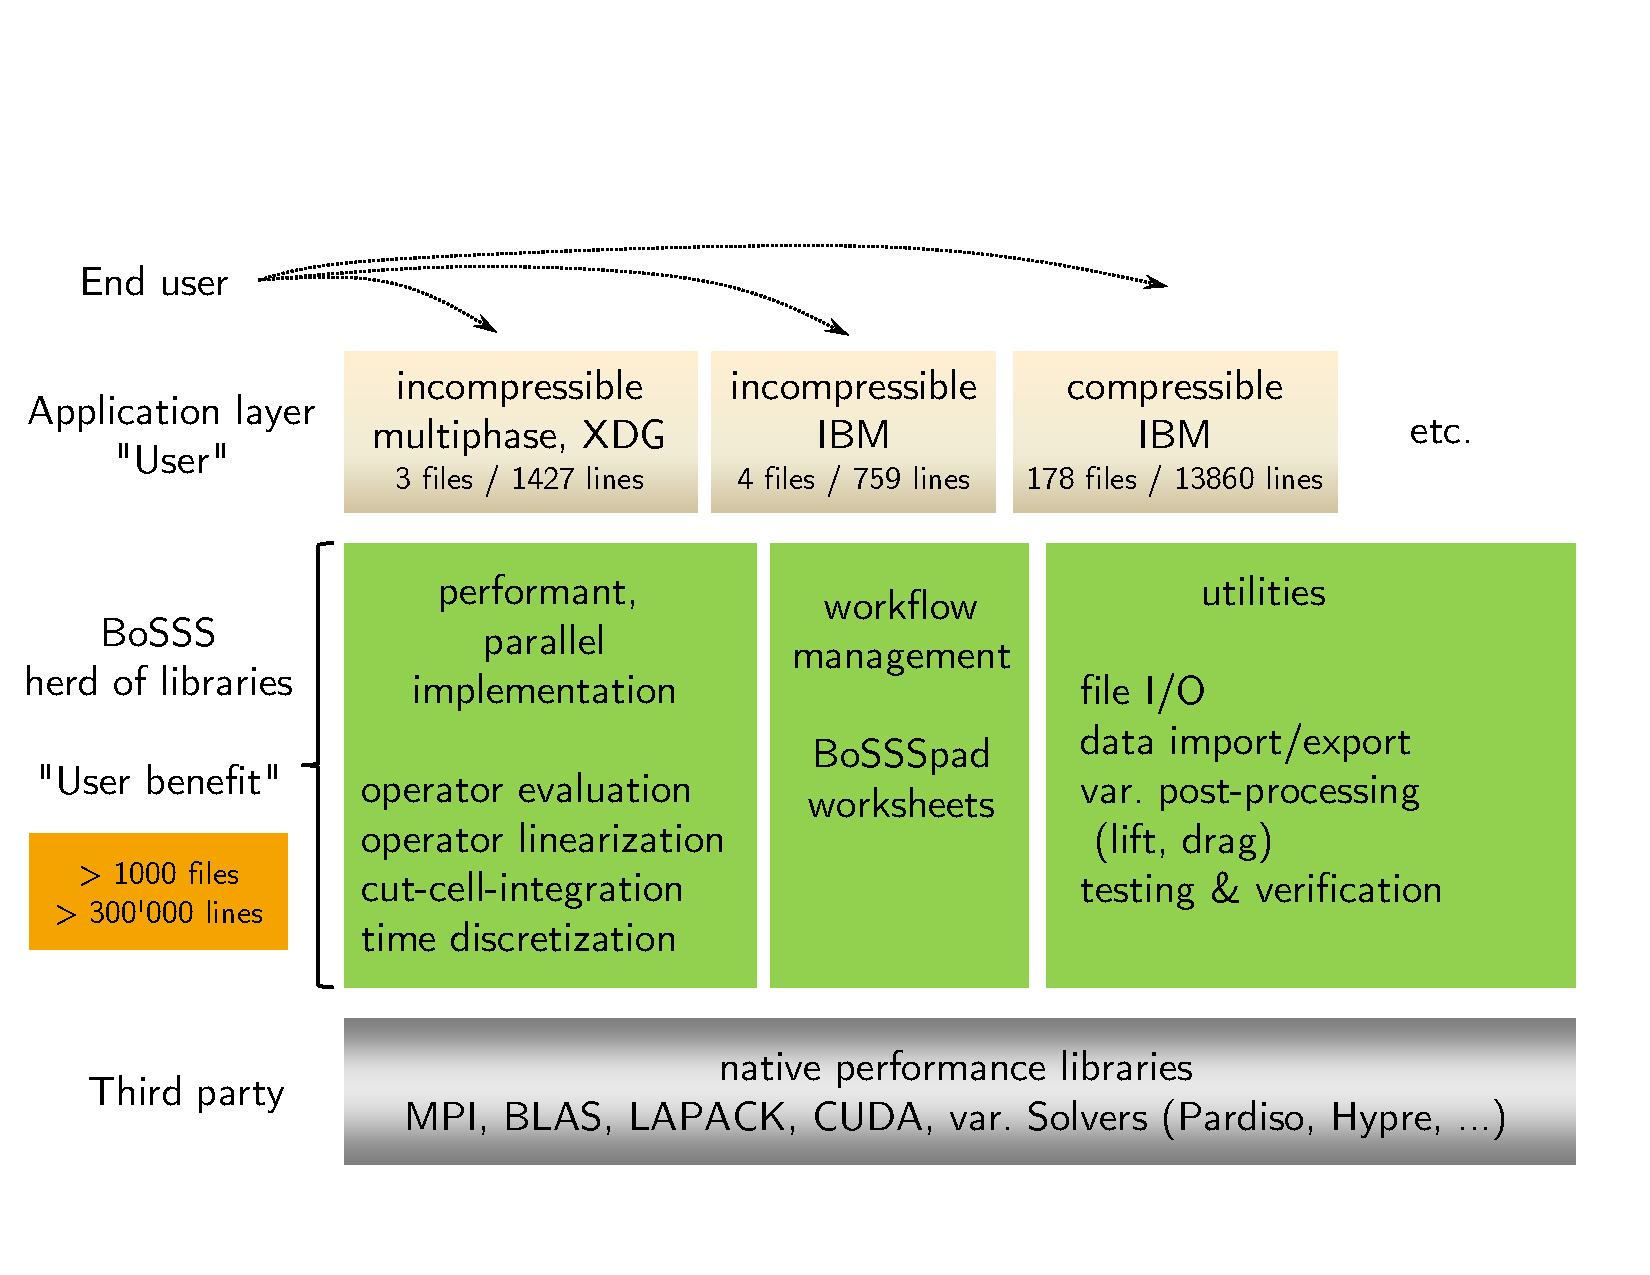
\includegraphics[width=\textwidth]{BoSSS-philosophy-1.pdf}
	\caption{Schematic representation of the structure of the BoSSS solver. Extracted from the BoSSS handbook \parencite{kummer2020}.}
	\label{Fig:BoSSS}
\end{figure}

\cleardoublepage
\chapter{Governing equations}	\label{ch:gov_eqs}
\glsresetall
The objective of this work is to present a methodology that allows the simulation of reactive fluids - with emphasis on combustion systems - making use of the low-Mach equations.  In this chapter, it is intended to show the governing equations used in this work to give some remarks regarding their derivation, as well the assumptions made within the present framework.


First, in \cref{sec:GovEqLowMach}, the governing equations that allow the description of reactive fluids are presented, in addition to other thermodynamic relationships, expressions for the transport parameters and the one-step chemical model. Subsequently, in \cref{ssec:NonDimLowMachEquations} the nondimensionalization of the equations is presented, as well as the low-Mach limit of the governing equations.

Finally, in \cref{sec:FlameSheet} the governing equations for an irreversible chemical model with an infinite reaction rate are presented. These equations are used as part of the algorithm to solve the finite reaction rate case.



\section{The low-Mach number equations for reactive flows} \label{sec:GovEqLowMach}
Combustion processes can be modeled by a system of non-linear partial differential equations, namely the balance equations for the total mass, momentum, energy, and mass of individual species (usually expressed in terms of mass fractions). This system needs to be solved together with an equation of state and expressions for the transport properties as well as for the chemical reaction rates.
The derivation of the governing equations for a reacting flow system can be found in the literature. For more information see for example the works from \textcite{keeChemicallyReactingFlow2003} and \textcite{poinsotTheoreticalNumericalCombustion2005}. In the following pages, the main ideas regarding the derivation of equations are presented. For a more detailed explanation,  the interested reader is referred to the cited works and the references therein.

\subsection{The reactive Navier--Stokes equations}\label{ssect:lowMachModel}
Throughout this work, variables with a hat sign, for example $\hat{\rho}$, represent dimensional variables, while those without it are nondimensional.  The derivation of the low-Mach number equations starts with the Navier--Stokes equations, the energy equation (in its temperature form), and the species transport equations.
Consider a reacting fluid mixture composed of $\gls{TotalNumberSpecies}$ species. Let $\hat{\vec{x}} =(\hat x, \hat y, \hat z)$ and $\hat t$ be the spatial vector and time. The primitive variables are the velocity field $\hat{\mathbf{u}} =(\hat u, \hat v, \hat w)$, the pressure $\hat p$, the temperature $\hat T$, and the mass fractions $Y_k$ of the $\gls{TotalNumberSpecies}$ total species. The set of governing equations to be solved is
\begin{subequations}
	\begin{align}
		%%%%%%%%%%%%%%%%%%%%%%%%%%%
		%%% Continuity
		%%%%%%%%%%%%%%%%%%%%%%%%%%%
		\label{eq:NS_Conti}
		 & \pfrac{\hat\rho}{\hat t} +\hat\nabla \cdot (\hat \rho \hat{\vec{u}})   = 0,                                                                                                                          \\%
		%%%%%%%%%%%%%%%%%%%%%%%%%%%
		%%% Momentum
		%%%%%%%%%%%%%%%%%%%%%%%%%%%
		\label{eq:NS_Momentum}
		 & \pfrac{\hat \rho \hat{\vec{u}}}{\hat t} +\hat\nabla \cdot (\hat \rho \hat{\vec{u}} \otimes  \hat{\vec{u}})   = - \hat\nabla \hat p - \hat \nabla \cdot \glsHat{ViscTensor}   -\hat\rho\hat{\vec{g}}, \\
		%%%%%%%%%%%%%%%%%%%%%%%%%%%
		%%% Energy (temperature)
		%%%%%%%%%%%%%%%%%%%%%%%%%%%
		\label{eq:NS_energy}
		%	\glsHat{dens}\glsHat{heatCapacity} \left(\pfrac{\glsHat{temp}}{\hat{t}} +\glsHat{velVec}\cdot \hat \nabla \hat{\gls{temp}}\right)
		 & \glsHat{dens}\glsHat{heatCapacity} \pfrac{\glsHat{temp}}{\hat{t}} +\glsHat{dens}\glsHat{heatCapacity} \glsHat{velVec}\cdot \hat \nabla \hat{\gls{temp}}
		= \Dfrac{\glsHat{TotalPress}} - \hat{\nabla}\cdot \hat{\vec{q}}
		-\left(\hat \rho \sum_{k = 1}^{\gls{TotalNumberSpecies}} \hat{c}_{p,k} Y_k \glsHat{velDiffusionvec}_k\right) \cdot \hat \nabla \glsHat{temp} %% Shouldi include this term?
		+\glsHat{ViscTensor}\colon\hat \nabla \glsHat{velVec} + \hat \omega_T,                                                                                                                                   \\
		%%%%%%%%%%%%%%%%%%%%%%%%%%%
		%%% Mass fraction k
		%%%%%%%%%%%%%%%%%%%%%%%%%%%
		\label{eq:NS_SpeciesBalance}
		 &                                                                                                                                                                                                      %	\pfrac{\hat \rho  Y_k }{\hat t} +	\hat\nabla \cdot (\hat \rho \hat{\vec{u}} Y_k)  & = \hat\nabla \cdot(\hat\rho\hat D_k \hat\nabla Y_k)+ 	  \hat \omega_k	  \quad (k = 1, \dots,~N - 1) \label{eq:GasLowMachMassBalance} 
		\pfrac{\hat \rho  Y_k }{\hat t} +	\hat\nabla \cdot (\hat \rho \hat{\vec{u}} Y_k)
		=  -	\hat\nabla \cdot \hat{\vec{j}}_k	 +  \hat{\gls{reactionRate}}  \quad (k = 1, \dots,~\gls{TotalNumberSpecies})
	\end{align}
	\label{eq:NS-eq}
\end{subequations}
In the general case this results in  $\gls{TotalNumberSpecies} + 5$ differential equations to be solved. In these equations, $\hat \rho$ is the density of the mixture and $\hat{\vec{g}}$ is the acceleration of gravity. $\glsHat{ViscTensor}$, $\hat{\vec{q}}$ and $\hat{\vec{j}}_k$ are the viscous tensor, the heat flux vector and the molecular mass flux vector of species $k$, respectively. Additionally, $\hat \omega_T$ is the heat release from combustion and $\hat \omega_k$ is the reaction rate of species $k$. To close the system, expressions must be defined to link these variables with the primitive variables. They will be briefly shown and commented upon in the following paragraphs.
\subsubsection{Equation of state}
Assuming that the fluid behaves ideally, the density can be calculated as
\begin{equation}
	\hat \rho = \frac{\hat{p}  \hat{W}_{\text{avg}}}{\mathcal{R} \hat{T} }. \label{eq:IdealGassDimensional}
\end{equation}
Here, $\hat{\gls{GasConstant}}$ is the universal gas constant of gases, and $\hat W_{\text{avg}}$ is the average molecular weight of the fluid, defined as
\begin{equation}
	\hat W_{\text{avg}} = \left( \SumOvAllns \frac{Y_k}{\hat W_k} \right)^{-1}
\end{equation}
with $\hat{\gls{MolecularWeight}}$ as the molecular weight of species $k$.  For an ideal mixture, the specific heat capacity can be calculated as a weighted average of the specific heats of the species 
\begin{equation}
	\hat c_p = \SumOvAllns Y_k \hat{c}_{p,k},%(\hat{T}),
\end{equation}
where $\hat{c}_{p,k}$ corresponds to the specific heat capacity of the component $k$. The temperature dependence of $\hat{c}_{p,k}$ can be accounted for by using NASA polynomials \parencite{mcbrideNASAThermodynamicData1993}
\begin{equation}
	\hat{c}_{p,k} = \left(\hat a_1 + \hat  a_2\glsHat{temp} +\hat  a_3\glsHat{temp}^2 +\hat  a_4\glsHat{temp}^3+\hat a_5\glsHat{temp}^4\right)\frac{\hat{\gls{GasConstant}}}{\hat{\gls{MolecularWeight}}},
\end{equation}
where $\hat a_1$, $\hat a_2$, $\hat a_3$, $\hat a_4$ and $\hat a_5$ are numerical coefficients supplied by the NASA database.
\subsubsection{Transport models}
The viscous tensor $\glsHat{ViscTensor}$ is defined for a Newtonian fluid as
\begin{equation}
	\glsHat{ViscTensor}= -\hat{\gls{visc}}\left( \hat\nabla \hat{\gls{velVec}} +(\hat\nabla\hat{\gls{velVec}})^T\right)  + \left(\frac{2}{3}\hat{\gls{visc}} - \hat \kappa \right) (\hat\nabla\cdot \hat{\gls{velVec}})\mytensor{I}.
\end{equation}
Here, $\hat{\gls{visc}}$ is the dynamic viscosity of the fluid, which is generally specific to the fluids and depends on its temperature and pressure. Furthermore, $\hat \kappa$ corresponds to the bulk viscosity, which is usually negligible for fluids at low pressures \parencite{birdTransportPhenomena1960}. In the rest of this work $\hat \kappa$ will be taken to be equal to zero.

The heat flux vector $\hat{\vec{q}}$ is given by Fourier's law of heat conduction,
\begin{equation}
	\hat{\vec{q}} = \hat \lambda \hat{\nabla} \glsHat{temp}.
	\label{eq:fourierLaw}
\end{equation}
Here, $\hat \lambda$ corresponds to the thermal conductivity, which, similar to viscosity, depends on the particular fluid under study as well as its temperature and pressure. Soret and Dufour effects are not considered in the present work.

The molecular mass flux vector $\hat{\vec{j}}_k$ of species $k$ is defined as $ \hat{\vec{j}}_k = \hat \rho \glsHat{velDiffusionvec}_k$, where $\glsHat{velDiffusionvec}_k$ is the diffusion velocity of the component $k$. In general, $\glsHat{velDiffusionvec}_k$ can be obtained by solving the Maxwell-Stefan equations
\begin{equation}
	\nabla X_p = \sum_{k=1}^{N}\frac{X_p X_k}{D_{pk}}(\vec{U}_k-\vec{U}_p), \qquad p = 1,\dots,N. \label{MaxwellStefan}
\end{equation}
Here $D_{pk} = D_{kp}$ is the binary mass diffusion coefficient of species $p$ into species $k$. $X_p$ is the mole fraction of species $k$ and is related to the mass fraction of $k$ as $ X_k = Y_k \hat W /\hat W_k$.
The solution of the system \eqref{MaxwellStefan} is often a difficult and costly task \parencite{williamsCombustionTheoryFundamental2000,poinsotTheoreticalNumericalCombustion2005}, and often simplifications are made. It can be shown that for binary mixtures ($N = 2$), and for mixtures containing multiple species ($N>2$), where all diffusion coefficients are equal, the system \eqref{MaxwellStefan} reduces exactly to the well-known Fick's law
\begin{equation}
	\hat{\vec{j}}_k = -\rho \hat D_k \nabla Y_k.
\end{equation}\label{eq:FickLaw}
This expression is exact only in the cases mentioned above. The variable $\hat D_k$ corresponds in this case to the diffusion coefficient of species $k$ in the mixture. An issue related to global mass conservation can be noted here. Recall that by definition, the sum of the mass fractions must always be one, namely $ \sum_{k=1}^{N}Y_k = 1$. This is only true for the solution of \cref{eq:NS-eq} if exact expressions for diffusion velocities are used \parencite{poinsotTheoreticalNumericalCombustion2005}. If some inexact expression is used (as, for example, Fick's law), the constraint for the sum of the mass fractions will not be fulfilled. This problem can be solved by solving the global mass conservation (continuity) equation \cref{eq:NS_Conti} and only the equations for the first $\gls{TotalNumberSpecies} - 1$ species \cref{eq:NS_SpeciesBalance}.
Therefore, all inconsistencies originating from not using an exact species diffusion model are absorbed by $Y_{\gls{TotalNumberSpecies}}$. As pointed out in \textcite{poinsotTheoreticalNumericalCombustion2005}, this simplification should only be used if all $\gls{TotalNumberSpecies}-1$ species are strongly diluted in species $\gls{TotalNumberSpecies}$, such as the case of a flame in air, where the mass fraction of nitrogen is large. It can also be noted that this approach reduces the number of differential equations needed to be solved by one.

The temperature dependence of viscosity is modeled by Sutherland's law \parencite{sutherlandLIIViscosityGases1893}
\begin{equation}\label{eq:DimSutherland}
	\hat{\mu}(\hat{T}) = \hat{\mu}_{\text{suth}}\left(\frac{\hat{T}}{\hat{T}_{\text{suth}}}\right)^{1.5}\frac{\hat{T}_{\text{suth}} + \hat{S}}{\hat{T}+\hat{S}}.
\end{equation}
Here $\hat{\mu}_{\text{suth}}$ is the viscosity evaluated at a reference temperature $\hat{T}_{\text{suth}}$, and $\hat S$ is a material-dependent parameter. In all calculations in this work, the value of $\hat{S}$ for air is used, i.e. $\hat{S} = $ \SI{110.5}{\kelvin}. Expressions for determining the thermal conductivity and diffusion coefficients as a function of temperature can be obtained using similar expressions, as shown later in \cref{ssec:NonDimLowMachEquations}.

The enthalpy transport term due to diffusive fluxes (third therm on the right hand side of \cref{eq:NS_energy}) usually has only a small influence on the solution (\textcite{smokeFormulationPremixedNonpremixed1991, goeyModelingSmallScale1995,paxionDevelopmentParallelUnstructured2001}), and it is actually exactly equal to zero for systems where all species heat capacities are equal. In the present formulation this term is neglected in the energy equation. 
%by assuming constant values for the Prandtl and Lewis numbers (to be defined later), we obtain expression for the temperature dependency of the other transport parameters as $\hat{k}/\hat{c}_p(\hat T) = \hat \mu/\text{Pr}$ and $\hat \rho \hat D_k(\hat T) = \hat \mu/\text{Pr}\text{Le}_k$.

\subsubsection{Chemical model}
Consider a system composed of $N$ species where $M$ chemical reactions take place. Chemical reactions can be written in generalized form as follows.
\begin{equation}\label{eq:allChemEq}
	\sum_{k=1}^{N} \nu'_{kj}\mathcal{M}_k  \rightleftharpoons \sum_{k=1}^{N} \nu''_{kj}\mathcal{M}_k  \qquad \text{for}\qquad j=1,\dots,M\, ,
\end{equation}
where $\nu'_{jk}$ and $\nu''_{jk}$ are the molar stoichiometric coefficients of species $k$ in the chemical reaction $j$, and $\mathcal{M}_k$ represents the chemical component $k$. \newline

%%%%%%%%
The reaction rate of species $k$ is $\hat \omega_k$, which accounts for the total amount of species $k$ that appear or disappear due to $M$ chemical reactions (c.f. Equations \eqref{eq:allChemEq}). Its given by
\begin{equation} \label{eq:reacRateDef}
	\hat \omega_k  = \hat W_k \sum_{j=1}^{M}\nu_{jk}\hat{\mathcal{Q}}_j.
\end{equation}
Here $\nu_{kj} = \nu''_{kj} -\nu'_{kj}$, and $\mathcal{Q}_j$ is the rate of progress of the reaction $j$. They are usually modeled using Arrhenius-type expressions.\newline

%%%%%%%
The heat release $\hat \omega_T$ that appears in the energy equation is related to the reaction rates according to
\begin{equation}\label{eq:heatRelDef}
	\hat \omega _T = - \sum_{k=1}^{N} \hat h_k\hat\omega_k = - \sum_{k=1}^{N}   \Delta \hat h_k^0 \hat\omega_k   - \sum_{k=1}^{N} \hat h_{ks} \hat\omega_k.
\end{equation}
Here, the specific enthalpy of $k$-th species $\hat h_k$  is written in terms of its formation enthalpy $\hat h_k^0$ and a sensible enthalpy $\hat h_{ks} =\int_{0}^{\hat{T}} \hat c_{p,k} \text{d}\hat{T} $. The second term on the right-hand side of \cref{eq:heatRelDef} is usually small and is exactly zero for a mixture where all the heat capacities of each component are equal \parencite{poinsotTheoreticalNumericalCombustion2005}. It will be neglected in the rest of the analysis.
\newline

In this work,  the one-step kinetic model for the combustion of hydrocarbons presented in \textcite{fernandez-tarrazoSimpleOnestepChemistry2006} is used. The chemical reaction is represented by a single ($M = 1$)  exothermic global irreversible expression as
\begin{equation}
	\ch{C}_n \ch{H}_m + \left(n+\frac{m}{4}\right) \ch{O}_2\ch{ -> } n \ch{CO2} + \frac{m}{2} \ch{H2O}.
\end{equation}%TODO \todo{correct boldletter}
The rate of progress of the global reaction is modeled by an Arrhenius-type expression
\begin{align}
	\hat{\mathcal{Q}}= \hat B e^{-\hat T_a/\hat T} \left(\frac{\hat \rho Y_F}{\hat W_F}\right)^a \left(\frac{\hat \rho Y_O}{\hat W_O}\right)^b . \label{eq:DimArr}
\end{align}%
Here, the subscripts $F$ and $O$ refer to fuel and oxidizer, respectively. The parameter $\hat{B}$ corresponds to the pre-exponential factor, $\hat T_a$ is the activation temperature, and $a$ and $b$ are reaction orders. For a one-step reaction model, the reaction rate of the $k$-th component in\cref{eq:reacRateDef} is
\begin{equation}
	\hat \omega_k  =  \nu_{k} \hat W_k\hat{\mathcal{Q}}.
\end{equation}
With this definition, the heat release $\hat \omega_T$ in \cref{eq:heatRelDef} yields
\begin{equation}
	\hat \omega_T = - \hat W_F \hat \omega_F\hat Q^m = - \hat \omega_F\hat Q .
\end{equation}
Here $\hat Q^m$ is the molar heat of reaction of the one-step reaction and $\hat Q$ is the mass heat of reaction. $\hat W_F$ and $ \hat \omega_F$ are the molar mass of the fuel species and the reaction rate of the fuel species respectively.

\begin{table}[!btp]
	\centering
	\begin{tabular}{
			@{}
			S[table-format=4.2]
			S[table-format=7.2]
			S[table-format=1]
			S[table-format=1]
			S[table-format=2.2]
			@{}
		}
		\toprule
		{$\hat B$}                                         &
		{$\hat{T}_{a0}$}                                   &
		{$\hat{\heatRelease}_0$}                           &
		{$a$}                                              &
		{$b$}                                                \\
		{$(\si{\centi\metre\cubed\per(\mole\, \second)})$} &
		{$(\si{\kelvin})$}                                 &
		{$(\si{\mega \joule \per \kilo \mole})$}           &
		{}                                                 &
		{}                                                   \\
		\midrule
		${6.9\times 10^{14}}$                              &
		15900                                              &
		802.4                                              &
		1                                                  &
		1                                                    \\
		\bottomrule
	\end{tabular}
	\caption{Base parameters used in the one-step combustion model by \textcite{fernandez-tarrazoSimpleOnestepChemistry2006}}\label{Tab:OneStepParameters}
\end{table}%

Within the model from \textcite{fernandez-tarrazoSimpleOnestepChemistry2006}, several parameters are adjusted to represent characteristic features of premixed flames and diffusion flames. The parameters $\hat T_a$ and $\hat \heatRelease$ are defined as functions of the local equivalence ratio $\phi$, which is, in turn, defined in terms of the local mass fractions of fuel $Y_F$ and oxidizer $Y_O$ as
\begin{equation}\label{eq:equivalenceRatio}
	\phi = \frac{s Y_F^0}{Y_O^0}\frac{s Y_F-Y_O+Y_O^0}{s(Y_F^0-Y_F) + Y_O},
\end{equation}
where $Y_F^0$ and $Y_O^0$ are the mass fractions of the fuel and oxidizer flows in their corresponding feed streams, and $s$ is the mass stoichiometric ratio, defined as $s =\nu_O \hat W_O/\nu_F \hat W_F$.
The activation energy depend on $\phi$ as
\begin{equation}
	\hat{T}_a(\phi)=
	\begin{cases}
		(1 + 8.250(\phi-0.64)^2) \hat{T}_{a0} & \text{if}~ 	\phi \leq 0.64,           \\
		\hat{T}_{a0}                          & \text{if}~ 	0.64 \leq \phi \leq 1.07, \\
		(1 + 4.443(\phi-1.07)^2)\hat{T}_{a0}  & \text{if}~\phi \geq 1.07,
	\end{cases} \label{eq:ActivationTemperatureOneStep}
\end{equation}
and the molar heat release according to
\begin{equation}
	\hat{\heatRelease}(\phi)=
	\begin{cases}
		\hat{\heatRelease}_0                      & \text{if}~ \phi \leq 1, \\
		(1 - \alpha(\phi -1))\hat{\heatRelease}_0 & \text{if}~\phi > 1.
	\end{cases}  \label{eq:heatReleaseOneStep}
\end{equation}

The parameter $\alpha$ is a constant that depends on the hydrocarbon being considered, in particular $\alpha = 0.21$ for methane combustion.

It should be noted that \cref{eq:heatReleaseOneStep} yields unphysical values of $\hat Q$ for large values of $\phi$. This problem can be avoided by setting an upper boundary value for $\phi$ in \cref{eq:heatReleaseOneStep}. However, in practice, this should not have a significant effect because the non-physical values of $\hat Q$ appear in zones where the reaction rate $\hat{\rateReac}$ is very close to zero, making the factor $\hat Q \hat{\rateReac}$ in the temperature equation negligible. However, setting an upper bound for $\phi$ is helpful in avoiding possible numerical instabilities.
%%%%%%%%%%%%%%%%%%%%%%%%%%%%%%%%%%%%%%%%%%%%%%%%%%%%%%
%%%%%%%%%%%%%%%%%%%%%%%%%%%%%%%%%%%%%%%%%%%%%%%%%%%%%%

\subsection{The reactive low-Mach Navier-Stokes equations} \label{ssec:NonDimLowMachEquations}

In the present work, the low-Mach number approximation of the governing equations is used. The derivation of the equations can be found in the works from \textcite{rehmEquationsMotionThermally1978, majdaDerivationNumericalSolution1985,mullerLowMachNumberAsymptoticsNavierStokes1998}. The interested user is referred to these references for a detailed explanation of how the set of equations is derived. In what follows, the main consequences of the low Mach limit will be shown and discussed.

Recall the definition of the Mach number, $\text{Ma} = \RefVal{u}/\hat c$, where $\RefVal{u}$ is a characteristic flow velocity and $\hat{c}$ the speed of sound. The low-Mach number limit approximation of the governing equations is used for flows where the Mach number is small, which is usually the case in typical laminar combustion systems \parencite{dobbinsFullyImplicitCompact2010}.
The low-Mach equations are obtained by using standard asymptotic methods. One of the main results of the analysis is that for flows with a small Mach number, the pressure can be decomposed as
\begin{equation}
	\hat p(\hat {\vec{x}}, \hat t) = \underbrace{\hat p_0(\hat t)}_{\mathcal{O}(1)} + \underbrace{\hat p_2(\hat{\vec{x}},\hat t)}_{\mathcal{O}(\text{Ma}^2)} .
\end{equation}
The spatially uniform term $\hat p_0(\hat t)$ is called thermodynamic pressure and only influences the system through the equation of state. It is constant in space but can change in time.  For an open system, the thermodynamic pressure is also constant in time and equal to the ambient pressure, while for a closed system (e.g. a system completely bounded by walls) it changes in order to ensure mass conservation. 

On the other hand, the perturbational term $\hat p_2(\hat{\vec{x}},\hat t)$ appears only in the momentum equations and plays a role similar to that of the pressure in the classical incompressible formulation. This perturbational term satisfies $\hat p_2/\hat p \sim \mathcal{O}(\text{Ma})^2$ \parencite{dobbinsFullyImplicitCompact2010,nonakaConservativeThermodynamicallyConsistent2018} showing that  the equation of state is satisfied only to $\mathcal{O}(\text{Ma}^2)$.

Effectively, the low-Mach limit of the Navier-Stokes equations allows the calculation of systems where large density variations due to temperature differences are present, thus the formulation is not restricted to approximations such as the Boussinesq approximation for buoyancy-driven flow. In addition, this approximation truncates the mechanism of pressure wave propagation, which is a natural feature of the compressible Navier-Stokes equations. By doing this the necessity of small time-steps for resolving the wave phenomenon is completely removed and the maximum allowed time-step is greatly increased.

In this work a nondimensional formulation of the governing equations is used. Following nondimensional quantities are defined
\begin{align*}
	      & \rho = \frac{\hat \rho}{\RefVal{\rho}}, \quad
	p = \frac{\hat p}{\RefVal{p}}, \quad
	\vec{u}= \frac{\hat{\vec{u}}}{\RefVal{u}}, \quad
	T = \frac{\hat T}{\RefVal{T}},  \quad
	c_p = \frac{\hat c_p}{\RefValS{c}{p}}, \quad
	W_k = \frac{\hat{W}_k}{\RefVal{W}},
	\\
	\mu = & \frac{\hat \mu}{\RefVal{\mu}},\quad
	D_k = \frac{\hat D_k}{\RefValS{D}{k}}, \quad
	k = \frac{\hat k}{\RefVal{k}}\quad
	\nabla = \frac{\hat \nabla}{\RefVal{L}}, \quad
	t = \frac{\hat{t}}{\RefVal{t}},\quad
	\vec{g} = \frac{\hat{\vec{g}}}{\RefVal{g}},\quad
	Q = \frac{\hat Q}{\hat{Q}_0}.
\end{align*}
Here $\RefVal{u}, \RefVal{L}$, $\RefVal{p}$, $\RefVal{t}$, and $\RefVal{T}$ are the reference velocity, length, pressure, time, and temperature, respectively, and are equal to some characteristic value for the particular studied configuration. Furthermore, $\RefVal{g}$ is the magnitude of the gravitational acceleration and $\RefVal{W}$ is the reference molecular weight. The reference transport properties $\RefVal{\mu}$, $\RefVal{k}$, $\RefValS{D}{k}$ and the reference heat capacity of the mixture $\RefValS{c}{p}$ are evaluated at the reference temperature $\RefVal{T}$. Similarly, the reference density must satisfy the equation of state, thus $\RefVal{\rho} = \RefVal{p}/(\hat{\mathcal{R}}\RefVal{T}\RefVal{W})$.  By introducing these definitions into the governing  \cref{eq:NS_Conti,eq:NS_Momentum,eq:NS_energy,eq:NS_SpeciesBalance} the reactive set of nondimensional low-Mach number equations is obtained. The system of differential equations to be solved reads as follows.
\begin{subequations}
	\begin{align}
		 & \pfrac{\rho}{t} + \nabla \cdot (\rho \vec{u})   = 0, \label{eq:LowMach_Conti}                                                                                                                                                                                                   \\
		 & \pfrac{\rho \vec{u}}{t} + \nabla \cdot (\rho \vec{u} \otimes \vec{u})   = - \nabla p + \frac{1}{\Rey}\nabla \cdot \mu\left( \nabla \vec{u} +\nabla \vec{u}^T  - \frac{2}{3}(\nabla\cdot \vec{u})\mytensor{I} \right)  - \frac{1}{\Fr^2}\rho\vec{g}, \label{eq:LowMach_Momentum} \\
		 &\frac{1}{\gamma} \pfrac{\rho T}{t} + \nabla \cdot (\rho \vec{u} T)  = \frac{1}{\text{Re}~\text{Pr}}\nabla \cdot\left(\frac{k}{c_p} \nabla T\right)+ \text{H}~\Da~\frac{\heatRelease~\mathcal{Q}}{c_p}, \label{eq:LowMachEnergy}                                                                  \\
		 & \pfrac{\rho Y_k}{t} +	\nabla \cdot (\rho  \vec{u}Y_k)   = \frac{1}{\text{Re}~\text{Pr}~\text{Le}_k}\nabla \cdot(\rho D \nabla Y_k)+  \Da~\stoicCoef_k W_k \mathcal{Q}, \quad k = 1, \dots,~N - 1. \label{eq:LowMachMassBalance}
	\end{align}
	\label{eq:all-eq}\label[pluralequation]{eq:all-eqs}
\end{subequations}
This system is solved for the primitive variables velocity $\vec{u} = (u_x, u_y)$, pressure $p$, temperature $T$ and mass fractions ${\mathbf{Y}' = (Y_1,\dots,Y_{N-1})}$. Note that it is assumed that the spatial gradients of the mixture heat capacity are small, which allows to introduce $c_p$ in the derivative of the diffusive term of \cref{eq:LowMachEnergy}. Furthermore, considering the fact that the sum of the mass fractions must always be one, the mass fraction of the last species $\gls{TotalNumberSpecies}$ can be calculated with
\begin{align} \label{eq:MassFractionConstraint}
	Y_{\gls{TotalNumberSpecies}} = 1 - \sum_{k = 1}^{\gls{TotalNumberSpecies}-1}Y_k.
\end{align}
Note that the form of the low-Mach equations is very similar to the Navier-Stokes equations. The major difference is in the decomposition of the pressure. This similarity is beneficial as it allows the use of similar techniques to solve the PDE system to those used for the completely incompressible case \parencite{keshtibanCompressibleFlowSolvers2003}. From now on, the sub-index of the hydrodynamic pressure $\hat p_2$ will be dropped and it will be called simply $\hat p$, further emphasizing the similarity in its role to the pressure of the incompressible equations.

Six nondimensional factors arise from the nondimensionalization process:
\begin{gather*}
	\text{Re} = \frac{\RefVal{\rho} \RefVal{u}  \RefVal{L}}{\RefVal{\Viscosity}}, \quad
	\text{Fr} = \frac{\RefVal{u}}{\sqrt{\RefVal{g}\RefVal{L}}}, \quad
	\text{Pr} = \frac{\RefValS{c}{p} \RefVal{\Viscosity}}{\RefVal{k}},\\%, \quad
	% \text{Ma} = \frac{\RefVal{u}}{\sqrt{\gamma \RefVal{T} \hat{\gls{GasConstant}} / \RefVal{W} }},\\
	\text{Le}_k = \frac{\RefVal{k}}{\RefVal{\rho} \RefValS{D}{k} \RefValS{c}{p}}, \quad
	\Da = \frac{\hat B \RefVal{L} \RefVal{\rho}}{\RefVal{M}\RefVal{u}}, \quad \label{eq:Dahmkoeler}
	\text{H} = \frac{\hat \heatRelease_0}{\RefValS{c}{p}. \RefVal{T}}%%%%%%%%%%%%%%%%%%%%%%% CHECK THIS,  not sure if \RefVal{M} should be here
	%\text{H} = \frac{\hat \heatRelease_0}{\RefVal{M} \RefValS{c}{p} \RefVal{T}}%%%%%%%%%%%%%%%%%%%%%%% CHECK THISONEEEEEEEEEEEEEEEEEEEEE
\end{gather*}
The first three equations define the Reynolds, Froude and Prandtl number, respectively. $\text{Le}_k$ is the Lewis number of species $k$. Finally, $\text{Da}$ and H are the Damköhler number and the nondimensional heat release, respectively. The nondimensional progress of the global reaction reads as follows
\begin{align}
	\mathcal{Q}(T, \vec{Y})  = \left(\frac{\rho Y_F}{M_F}\right) \left(\frac{\rho Y_O}{M_O}\right)\text{exp}\left(\frac{-T_a}{T}\right), \label{eq:NonDimArr}
\end{align}
where $T_a = \hat{T}_a / \RefVal{T}$. Furthermore, the nondimensional heat release is
\begin{equation}
	\heatRelease(\phi)=
	\begin{cases}
		1                     & \text{if}~ \phi \leq 1, \\
		(1 - \alpha(\phi -1)) & \text{if}~\phi > 1.
	\end{cases}  \label{eq:heatReleaseOneStepNonDim}
\end{equation}
with $\phi$ evaluated according to \cref{eq:equivalenceRatio}. In the low-Mach limit, the ideal gas equation depends on the thermodynamic pressure, temperature and mass fractions. It reads in its nondimensional form
\begin{align} \label{eq:ideal_gas}
	\rho(p_0,T, \vec{Y}) = \frac{p_0}{T \SumOvAllns \frac{Y_k}{W_k}}.
\end{align}
As mentioned above, the thermodynamic pressure of a closed system is a parameter that has to be determined (for an open system is equal to the atmospheric pressure). By integrating \cref{eq:ideal_gas} into the entire domain $\Omega$, the expression
\begin{equation}
	p_0(T, \vec{Y}) = \frac{m_0}{\int_\Omega \left( T\sum_{k=1}^{N} \frac{Y_k}{W_k} \right)^{-1}\text{d}V} \label{eq:p0Condition}
\end{equation}
can be derived. Here, $m_0 = \int_\Omega \rho \text{d}V$ is the mass of the fluid in the closed system. Since in a closed system the total mass is constant, it can be determined using initial conditions.
Similarly, the nondimensional specific heat capacity of the mixture $c_p$ is calculated as
\begin{equation}\label{eq:nondim_cpmixture}
	c_p(T,\mathbf{Y}) = \SumOvAllns Y_k c_{p,\alpha},
\end{equation}
and the nondimensional viscosity as
\begin{equation} \label{eq:nondim_sutherland}
	\mu(T) =  T^{\frac{3}{2}}\frac{1+\hat{S} }{\RefVal{T}T+\hat{S}}.
\end{equation}
The model for the transport parameters can be simplified by assuming constant values for the Prandtl and Lewis numbers \parencite{smokeFormulationPremixedNonpremixed1991}.  The nondimensional transport parameters are related in that case with 
\begin{equation}
    \mu = k/c_p = \rho D.
\end{equation}
%%%%%%%%%%%%%%%%%%%%%%%%%%%%%%%%%%%%
%%%%%%%%%%%%%%%%%%%%%%%%%%%%%%%%%%%%
\subsection{A note on the multiple solutions of the system}
The system of equations shown in this section has the particularity that it presents branching phenomena, which means that there are several solutions to the problem. One solution is evidently that of pure mixing (also called frozen chemistry), in which combustion does not occur and the equations are simply describing a mixing process. Another solution is that of a system under combustion, where the reaction takes place in a thin but finite reaction zone, in which the reactants can overlap. This phenomenon is usually represented by a bifurcation curve of the combustion process, as shown in \cref{fig:Sshaped}. in which the maximum temperature of the system is plotted for different Dahmköhler numbers. 
The graph also shows the extinction point. If a system is in the stable combustion branch, and the Da number begins to decrease there is a point where the chemical reaction is not sustainable, and the extinction phenomenon occurs. An example of this is the case of a candle that is blown out and extinguished.

The ignition phenomenon can be interpreted analogously. For a system where there is no chemical reaction (but mixing of the reactants), the increase of the Dahmköhler number eventually leads to ignition of the system, obtaining a flame that is in the stable combustion branch. An example of this would be when a lighter produces a flame as a result of a spark. 

In the next section a strategy is presented that allows to obtain systems of steady state combustion, which does not require the simulation of the ignition process. 
\begin{figure}[h]
	\begin{center}
		\def\svgwidth{0.5\textwidth}
		\import{./plots/}{SShapedResponse.pdf_tex}
		\caption{S-shaped bifurcation curve of a combustion process.}
		\label{fig:Sshaped}%
	\end{center}%
\end{figure}%



\section{The flame sheet approximation} \label{sec:FlameSheet}

A problem encountered when numerically solving the system of  \cref{eq:LowMach_Conti,eq:LowMach_Momentum,eq:LowMachEnergy,eq:LowMachMassBalance} for the steady state simulation of combustion, is that the lack of suitable initial conditions can lead the algorithm to very slow convergence or even failure.  In this section, the concept of the flame sheet approximation is introduced, which is used for circumvent this problem. The ideas proposed in the work of \textcite{keyesFlameSheetStarting1987} are followed.

Assuming that all species have the same heat capacity $c_{p,k} = c_p$ and mass diffusion coefficient $D_k=D$, that the Lewis number is unity for all species, and that combustion can be described by a single step chemical reaction, it is possible to obtain an equation for a scalar without source terms, which is a linear combination of the energy \cref{eq:LowMachEnergy} and mass fraction \cref{eq:LowMachMassBalance}. Thus, the system can be simplified to solving the low-Mach Navier-Stokes equations and an equation for a scalar $z$:
\begin{subequations}
	\begin{flalign}
		&\pfrac{\rho}{t}+	\nabla \cdot (\rho \vec{u})                           = 0,& \label{eq:MixtFracConti2}                                                                                                                                                                    \\	
		&\pfrac{\rho \vec{u}}{t} +	\nabla \cdot (\rho \vec{u} \otimes \vec{u})  = - \nabla p + \frac{1}{\Rey}\nabla \cdot \mu\left( \nabla \vec{u} +\nabla \vec{u}^T  - \frac{2}{3}(\nabla\cdot \vec{u})\mytensor{I} \right)  - \frac{1}{\Fr^2}\rho\vec{g},&\label{eq:MixtFracMom} \\
		&\pfrac{\rho z}{t}+	\nabla \cdot (\rho \vec{u}z)                        = \frac{1}{\text{Re Pr}}\nabla \cdot\left(\rho D \nabla z\right).& \label{eq:MixtFracMF}
	\end{flalign}
	\label{eq:all-eq-mixfrac}
\end{subequations}
Note that \cref{eq:MixtFracMF} is simply a diffusion-convection equation. It is however still coupled to the flame structure via the velocity fields and through the density (and indirectly to the temperature and mass fractions fields, as will be shown later).
The system of \cref{eq:MixtFracConti2,eq:MixtFracMom,eq:MixtFracMF} need to be solved together with the equation of state (\cref{eq:ideal_gas}) and expressions for the transport parameters (\cref{eq:nondim_sutherland}). 

Here $z$ is the mixture fraction, which is a scalar that measures the local fuel/oxidizer ratio  \parencite{poinsotTheoreticalNumericalCombustion2005}. The variable $z$ is per definition equal to unity in the fuel feed stream and equal to zero in the oxidizer feed stream. Note that the system is not closed, because $\rho$, $\mu$ and $\rho D$ are still functions of the temperature and mass fractions. These fields can be related to the mixture fraction using the Burke-Schumann flame structure concept \parencite{burkeDiffusionFlames1928}. 
The procedure described before for obtaining the equation for the mixture fraction $z$ leads to expressions that relate $z$ to the temperature $T$, mass fraction of the fuel $Y_F$ and the mass fraction of the oxidizer $Y_O$ as
\begin{equation}
	z = \frac{s Y_F -Y_O +Y_O^0}{sY_F^0+Y_O^0} = \frac{\frac{c_p}{Q}(T-T_O^0)+Y_F }{\frac{c_p}{Q}(T_F^0-T_O^0)+Y_F^0} = \frac{\frac{s c_p}{Q}(T-T_O^0)+Y_O-Y_O^0 }{\frac{sc_p}{Q}(T_F^0-T_O^0)+Y_O^0} \label{eq:AllMFRelationships}
\end{equation}
In the case of an infinitely fast chemical reaction, fuel and oxidizer cannot coexist. On one side of this sheet only oxidizer is found, and on the other side only fuel. The exact position of the flame sheet can be determined  using \cref{eq:AllMFRelationships} by the location of the points where the reactant mass fractions $Y_F$ and $Y_O$ are zero, that is, the points where the mixture fraction $z = z_{st}$, with
\begin{equation}
	z_{st} = \frac{Y_O^0}{Y_O^0+sY_F^0}.
\end{equation}
Here $Y_O^0$ is the mass fraction of the oxidizer in the oxidizer inlet stream, and $Y_F^0$ is the mass fraction of fuel in the fuel inlet stream.
The Burke-Schumann flame structure provides analytical expressions for temperature and mass fraction fields on either side of the flame sheet as a function of the mixture fraction $z$. For a more detailed derivation see for example the textbook from \textcite{poinsotTheoreticalNumericalCombustion2005} or the work from \textcite{keyesFlameSheetStarting1987}.
The temperature is related to the mixture fraction as
\begin{equation}\label{eq:BS-T}
	T(z) =
	\begin{dcases}
		z T_F^0 + (1-z)T_O^0 + \frac{Q Y_F^0}{c_p}z_{st}\frac{1 - z}{1-z_{st}} & \text{if}\quad z \geq z_{st}, \\
		z T_F^0 + (1-z)T_O^0 + \frac{Q Y_F^0}{c_p}z                            & \text{if}\quad z < z_{st}.
	\end{dcases}
\end{equation}
The mass fraction field of fuel and oxidizer species at either side of the flame is given by:
\begin{equation}\label{eq:BS-YF}
	Y_F(z) =
	\begin{dcases}
		Y_F^0\frac{z - z_{st}}{1-z_{st}} & \text{if}\quad z \geq z_{st}, \\
		0                                & \text{if} \quad z < z_{st},
	\end{dcases}
\end{equation}
\begin{equation}\label{eq:BS-YO}
	Y_O(z) =
	\begin{dcases}
		0                                         & \text{if} \quad z \geq z_{st}, \\
		Y_O^0 \left( 1- \frac{z}{z_{st}}  \right) & \text{if} \quad z < z_{st}.
	\end{dcases}
\end{equation}
Finally, the mass fraction field of product species $P$ is:
\begin{equation}\label{eq:BS-YP}
	Y_P(z) =
	\begin{dcases}
		Y_O^0\frac{W_P\nu_P}{W_O\nu_O}(1-z) & \text{if} \quad z \geq z_{st}, \\
		Y_F^0\frac{W_P\nu_P}{W_F\nu_F}z     & \text{if} \quad z < z_{st}.
	\end{dcases}
\end{equation}
Once the mixture fraction field $z$ is obtained, the temperature and mass fraction fields are uniquely defined by \cref{eq:BS-T,eq:BS-YF,eq:BS-YO,eq:BS-YP}, which are used to evaluate the density and the transport properties. 


\begin{figure}[t]
	\pgfplotsset{
		group/xticklabels at=edge bottom,
		%		legend style = {
			%			at ={ (1.0,1.0), anchor= north west}
			%		},
		unit code/.code={\si{#1}}
	}
	\centering
	\inputtikz{MFFRC1}%
	\inputtikz{MFFRC2}%	
	\caption{Temperature and fuel mass fraction profiles calculated in the center-line of a counter-flow flame configuration using finite chemistry (black) and the flame sheet approximation (green). }
	\label{fig:MixtureFraction_finiteRateComparison}
\end{figure}
Note that the expressions shown above are not differentiable at the stoichiometric point, which also means that the density and transport properties are not differentiable at $z =z_{st}$. This presents a challenge for algorithms for finding solutions of the system \parencite{rauwoensConservativeDiscreteCompatibilityconstraint2009}. Later in \cref{ssec:MethodCombustion} this point will be treated.

The main idea of introducing the system of equations presented in this section is to obtain an adequate initial estimate that can be used to find a solution for the steady state systems with a finite reaction rate (\cref{eq:LowMach_Conti,eq:LowMach_Momentum,eq:LowMachEnergy,eq:LowMachMassBalance}). Note that the assumption of infinite reaction rate can be interpreted as an infinite Dahmköhler number, where the chemical time scales are much shorter than the flow scales. It is expected that the initial estimate using the flame-sheet is a good approximation for finite reaction rate systems where the Dahmköhler number is very large, or expressed differently, for conditions far away from the extinction point (see \cref{fig:Sshaped}).
Under certain conditions, the approximation is indeed very good. In \cref{fig:MixtureFraction_finiteRateComparison}, temperature and fuel mass fraction fields obtained with infinite and finite reaction rate across the center-line of a counterflow flame configuration are shown. Clearly, both solutions are very similar, differing only in the area near the flame. However, this similarity is only valid under the assumptions made to derive \cref{eq:MixtFracMF}. In the case that the Lewis number is not equal to one, or that the heat capacities are not equal for each species, the finite-rate solution will differ slightly from that obtained with the infinite-reaction rate. It should be mentioned that the steady state solution of the full problem obtained with this approach can be used to initialize non-steady state systems, and could help to simulating reactive systems while avoiding the ignition process.





\section{Boundary conditions}
The following boundary conditions are imposed for the resolution of the finite reaction rate system (\cref{eq:LowMach_Conti,eq:LowMach_Momentum,eq:LowMachEnergy,eq:LowMachMassBalance}) and for the flame sheet problem (\cref{eq:MixtFracConti2,eq:MixtFracMom,eq:MixtFracMF}),
\begin{subequations}
	\begin{align}
		\Gamma_{\text{D}}:\quad
		 & \vec{u} = \vec{u}_{\text{D}},
		\,\,\,
		T = T_{\text{D}},
		\,\,\,
		Y_{k}, =Y_{k,{\text{D}}},
		\,\,\,
		z = z_{\text{D}},
		\label{eq:bc_d}                                                                                                                                                                                             \\
		\Gamma_{{\text{DW}}}:\quad
		 & \vec{u} = \vec{u}_{\text{D}},
		\,\,\,
		\nabla T \cdot \vec{n}_{\partial \Omega} = 0,
		\,\,\,
		\nabla Y_{k} \cdot  \vec{n}_{\partial \Omega}= 0,
		\,\,\,
		\nabla z \cdot \vec{n}_{\partial \Omega} = 0,
		\label{eq:bc_dn}                                                                                                                                                                                            \\
		\Gamma_{\text{N}}: \quad
		 & \left( -p \mathbf{I}	+ \left(\frac{\mu}{\Reynolds} \left(\nabla \vec{u} + (\nabla \vec{u})^T\right) - \frac{2}{3}\mu(\nabla \cdot \vec{u})\mathbf{I}\right)\right)\cdot  \vec{n}_{\partial \Omega} 	= 0,
		\,\,\,\notag                                                                                                                                                                                                \\
		 &
		\nabla T \cdot \vec{n}_{\partial \Omega} = 0,
		\,\,\,
		\nabla  Y_{k} \cdot \vec{n}_{\partial \Omega}= 0,
		\,\,\,
		\nabla z \cdot \vec{n}_{\partial \Omega} = 0,
		\label{eq:bc_O}                                                                                                                                                                                             \\
		\Gamma_{\text{ND}}:\quad
		 & \left( -p \mathbf{I}	+ \left(\frac{\mu}{\Reynolds} \left(\nabla \vec{u} + (\nabla \vec{u})^T\right) - \frac{2}{3}\mu(\nabla \cdot \vec{u})\mathbf{I}\right)\right)\cdot  \vec{n}_{\partial \Omega} 	= 0,
		\,\,\,\notag                                                                                                                                                                                                \\
		 & T = T_{\text{D}},
		\,\,\,
		Y_{k} =  Y_{k,{\text{D}}},
		\,\,\,
		z = z_{\text{D}}
		\label{eq:bc_OD}                                                                                                                                                                                            \\
		\Gamma_{P}:\quad
		 & \vec{u}(\vec{x}) = \vec{u}(\vec{x}'),
		\,\,\,
		T(\vec{x}) = T(\vec{x}'),
		\,\,\,
		Y_{k}(\vec{x}) =  Y_{k}(\vec{x}'),
		\,\,\,
		z(\vec{x}) = z(\vec{x}'),
		\label{eq:bc_P}
	\end{align}
\end{subequations}
where $k = (1,\dots,N-1)$ denotes the index of mass fractions. The boundary $\Gamma_\text{D}$ represents conditions for inlets and walls, with the velocity, temperature, mass fractions and mixture fraction defined as Dirichlet boundary conditions. Boundaries $\Gamma_\text{DW}$  are used to represent adiabatic walls, where the velocity is given as a Dirichlet boundary condition again, but with the gradients perpendicular to the wall of the transported scalars are set to zero. The boundary $\Gamma_\text{N}$ represent an outflow of the domain with homogeneous Neumann condition for all scalars. The boundary $\Gamma_{\text{ND}}$ also  represents an outlet boundary condition, but with Dirichlet boundary conditions for the scalars. Finally, the boundaries $\Gamma_P$ are periodic, where $\vec{x}$ and $\vec{x}'$ are periodic pairs in the domain.

\mycomment{
	%TODO cosas por poner en algun lado
}
\cleardoublepage
\chapter{Numerical methods}	\label{ch:introduction}
%\glsresetall

\section{The Discontinous Galerkin method}
\subsection{Spatial discretization} \label{ssec:SpatDiscretization}
We start by introducing some standard definitions and notation in the context of DG methods:\cite{kummerExtendedDiscontinuousGalerkin2017} \cite{kikkerFullyCoupledHighorder}
We define a computational domain $\Omega \subset \mathbb{R}^2$ with a polygonal and simply connected boundary $\partial \Omega$. Our numerical grid is then defined by the set of non-overlapping elements $\mathcal{K} = \{K_1, ..., K_N\}$ with a characteristic mesh size $h$, so that $\Omega$ is the union of all elements, i.e. $\Omega = \bigcup_{i=1}^N K_i$. We define  $\Gamma = \bigcup_j \partial K_j$ as the union of all edges (internal edges and boundary edges) and $\Gamma_I = \Gamma \setminus \partial \Omega$ as the union of all interior edges.
For each edge of $\Gamma$ a normal field $\myvector{n}_{\Gamma}$ is defined. Particularly on $\partial \Omega$ is defined as an outer normal and $\vec{n}_\Gamma = \vec{n}_{\partial\Omega}$.
For each field $\myvector{u} \in C^0\left(\Omega\setminus \Gamma_I\right)$ we define  $\myvector{u}^-$  and  $\myvector{u}^+$, which describe the information in the interior and exterior sides of the cell:
\begin{align}
	\myvector{u}^- & = \lim_{\xi \searrow 0} \myvector{u}\left(\myvector{x} - \xi \myvector{n}_{\Gamma}\right) \quad \text{for } \myvector{x}\in \Gamma   \\
	\myvector{u}^+ & = \lim_{\xi \searrow 0} \myvector{u}\left(\myvector{x} + \xi \myvector{n}_{\Gamma}\right) \quad \text{for } \myvector{x}\in \Gamma_I
\end{align}
The jump and mean values of $\myvector{u}$ on inner edges $\Gamma_I$ are defined as:
\begin{align}
	\llbracket \myvector{u} \rrbracket & = \myvector{u}^+-\myvector{u}^-                           \\
	\{\myvector{u}\}                   & = \frac{1}{2} \left(\myvector{u}^-+\myvector{u}^+\right).
\end{align}
while the jump and mean values on boundary edges $\partial \Omega$ are:
\begin{align}
	\llbracket \myvector{u} \rrbracket & = \myvector{u}^-  \\
	\{\myvector{u}\}                   & = \myvector{u}^-.
\end{align}
We define the broken polynomial space of total degree $k$ as
\begin{equation}
	\mathbb{P}_k(\mathcal{K}_h)= \{f \in L^2\left(\Omega\right); \forall K \in \mathcal{K}: f\vert_{K} \text{ is polynomial and deg}\left(f\vert_{K}\right)\leq k \}.
	\label{Eq:PolSpace}
\end{equation}
Additionally for $u \in \mathcal{C}^1(\Omega \setminus \Gamma)$ the broken gradient $\nabla_h u$ is defined as:
\begin{equation}
	\nabla_h u
	= \begin{cases}
		0
		 & \text{on }\Gamma  \\
		\nabla u
		 & \text{elsewhere }
	\end{cases}
\end{equation}
The broken divergence  $\nabla_h \cdot u$ is defined analogously. Finally, we define the function space for test and trial functions for $D_v$ dependent variables:
\begin{equation}
	\mathbb{V}_\myvector{k} = \prod_{i=1}^{D_v} \mathbb{P}_{k_i}(K_h)
	\label{Eq:Vspace}
\end{equation}
where $\myvector{k} = \left(k_1,...,k_{D_v}\right)$.


%%%%%%%%%%%%%%%%%%%%%%%%%%%%%%%%%%%%%%%%%%%%%%%%%%%%%%%%%%%%%%%%%%%%%%%%%%%%%%%%%%%%%%%%%%%%%%%%%%%%%%%%%%%%%%%%%%%%%%%%%%%%%%%%%%%%%%%%%%%%%%%%%

\subsection{Discretization for a DG Method}
\label{sec:discretDGmethod}

As an introductory example, following \textcite{hesthaven_nodal_2008}, we are considering the discretization of a general conservation law with a non-linear flux function $\gls{flux}(\gls{fprop})$ for a scalar quantity $\gls{fprop} = \gls{fprop}(\vectr{x},t)$ in $\gls{domain}$ and suitable Dirichlet boundary condition on $\gls{boundary} = \diri{\gls{boundary}}$ and a compatible initial condition $\gls{fprop}_0$. The problem statement reads
\begin{subequations}
	\begin{align}
		\pDeriv{\gls{fprop}}{t} + \div{\gls{flux}(\gls{fprop})} & = 0,                        & \vectr{x} \in  \gls{domain},    \label{eq:generalConservLaw} \\
		\gls{fprop}                                             & = \diri{\gls{fprop}},       & \vectr{x} \in \diri{\gls{boundary}},
		\label{eq:generalConservLawBC}                                                                                                                       \\
		\gls{fprop}(\vectr{x}, 0)                               & = \gls{fprop}_0(\vectr{x}), & \vectr{x} \in  \gls{domain}.
		\label{eq:generalConservLawIC}
	\end{align}
	\label{eq:generalConservLawProblem}
\end{subequations}
The goal is to find an approximate solution $\gls{fprop} = \gls{fprop}(\vectr{x},t)$ to $\gls{fprop}$ that fulfils the problem \eqref{eq:generalConservLawProblem}. Therefore, the problem domain $\gls{domain}$ is discretized by a numerical mesh $\gls{grid}$ and for each numerical cell $\gls{cell}_j$ we introduce the approximation by a local polynomial basis $\vectr{\gls{basis}}_j = (\gls{basis}_{j,l})_{l=1,...,\gls{NoDOFloc}} \in \gls{brknPspacek}(\{\gls{cell}_j\})$ with a cell-local support $\textrm{supp}(\vectr{\gls{basis}}_j) = \overline{\gls{cell}}_j$ as
\begin{equation}
	\gls{fprop}_j(\vectr{x},t) = \sum_{l=1}^{N_k} \tilde{\gls{fprop}}_{j,l}(t) \gls{basis}_{j,l}(\vectr{x}) = \tilde{\vectr{\gls{fprop}}}_{j}(t) \cdot \vectr{\gls{basis}}_{j}(\vectr{x}), \quad \vectr{x} \in \gls{cell}_j,
	\label{eq:localApprox}
\end{equation}
where the coefficients $\tilde{\vectr{\gls{fprop}}}_{j} = (\tilde{\gls{fprop}}_{j,l})_{l=1,...,\gls{NoDOFloc}}$ denote the unknowns or degrees of freedom (DOF) of the local solution in cell $\gls{cell}_j$. In this work a modal polynomial basis is used, which fulfils the orthogonality condition
\begin{equation}
	\int_{\gls{cell}_j}  \gls{basis}_{j,m} \gls{basis}_{j,n} \d{V} = \delta_{mn}
\end{equation}
with the Kronecker delta $\delta_{mn}$. Inserting the local approximation \eqref{eq:localApprox} into the conservation law \eqref{eq:generalConservLaw} results in a cell-wise residual
\begin{equation}
	R_j(\vectr{x},t) = \pDeriv{{\gls{fprop}}_j}{t} + \div{\gls{flux}({\gls{fprop}}_j)}, \quad \vectr{x} \in \gls{cell}_j. %, \forall \gls{cell}_j \in \gls{grid}.
	\label{eq:localRes}
\end{equation}
For a Galerkin method, the residual \eqref{eq:localRes} is minimized with respect to the same space as the ansatz functions, i.e. $\gls{brknPspacek}(\{\gls{cell}_j\})$. Thus, we demand for the test functions $\gls{testF}_{j,l} = \gls{basis}_{j,l}$ in each cell $\gls{cell}_j \in \gls{grid}$ that
\begin{equation}
	\int_{\gls{cell}_j} R_j \gls{testF}_{j,l} \d{V} = \int_{\gls{cell}_j}  \pDeriv{{\gls{fprop}}_j}{t} \gls{basis}_{j,l} + \div{\gls{flux}({\gls{fprop}}_j)} \gls{basis}_{j,l} \d{V} \stackrel{!}{=} 0, \quad \forall \vectr{\gls{basis}}_{j,l}.
	\label{eq:DGminimization}
\end{equation}
So, for each cell we end up with a linear system of $\gls{NoDOFloc}$ equations. However so far, no approximate global solution $\gls{fprop} \in \gls{domain}$ can be regained from the minimization in \eqref{eq:DGminimization}. The global solution is assumed to be a piecewise polynomial approximation
\begin{equation}
	\gls{fprop}(\vectr{x},t) \approx  \gls{fprop}(\vectr{x},t) = \bigoplus\limits_{j=1}^{J} {\gls{fprop}}_j(\vectr{x},t) = \sum_{j=1}^{J} \sum_{l=1}^{\gls{NoDOFloc}} \tilde{\gls{fprop}}_{j,l}(t) \gls{basis}_{j,l}(\vectr{x}) \in \gls{brknPspacek}(\gls{grid})
	\label{eq:globalApprox}
\end{equation}
defined as the direct sum of the $J$ local solutions ${\gls{fprop}}_j$ in \eqref{eq:localApprox}. Here, $\tilde{\gls{fprop}}_{j,l}$, with $j={1,...,J}$ and $l={1,...,\gls{NoDOFloc}}$, denote the total DOF, with $\gls{NoDOF} = J \cdot \gls{NoDOFloc}$, of the global approximate solution $\gls{fprop}$. In order to formulate a global DG method, the spatial term on the right-hand side of equation \eqref{eq:DGminimization} is rewritten in terms of boundary edge integrals $\forall \gls{cell}_j \in \gls{grid}$ using partial integration
\begin{equation}
	\int_{\gls{cell}_j}  \pDeriv{{\gls{fprop}}_j}{t} \gls{basis}_{j,l} \d{V} - \int_{\gls{cell}_j} \gls{flux}({\gls{fprop}}_j) \cdot \gradH{\gls{basis}}_{j,l} \d{V} + \oint_{\partial{\gls{cell}}_j} \left( \gls{flux}({\gls{fprop}}_j) \cdot {\gls{normal}}_j \right) \gls{basis}_{j,l} \d{S} = 0, \quad \forall \gls{basis}_{j,l},
	\label{eq:DGfluxFormulation}
\end{equation}
where ${\gls{normal}}_j$ represents the local outward pointing normal for cell ${\gls{cell}}_j$. Note that on the internal edges $\gls{edgeInt}$ the value of $\gls{flux}({\gls{fprop}}_j)$ is multiply defined. Therefore, a numerical flux $\gls{numflux}$ is introduced
\begin{equation}
	\gls{numflux}(\inn{{\gls{fprop}}_j}, \out{{\gls{fprop}}_j}, \gls{normalGam}) \approx \gls{flux}({\gls{fprop}}_j) \cdot {\gls{normal}}_j,
\end{equation}
that uniquely defines the resulting value of both neighbouring values, i.e. $\inn{{\gls{fprop}}_j}$ and $\out{{\gls{fprop}}_j}$ at internal edges $\gls{edgeInt}$. Summing over all cells ${\gls{cell}}_j$, the global minimization problem for $\gls{fprop}(\vectr{x},t), \vectr{x} \in \gls{domain}$ reads: Find $\gls{fprop} \in \gls{brknPspacek}(\gls{grid})$, such that $\forall \gls{testF} = \gls{basis} \in \gls{brknPspacek}(\gls{grid})$
\begin{equation}
	\int_{\gls{domain}}  \pDeriv{\gls{fprop}}{t} \gls{basis} \d{V} - \int_{\gls{domain}} \gls{flux}(\gls{fprop}) \cdot \gradH{\gls{basis}} \d{V} + \oint_{\gls{edge}} \gls{numflux}(\inn{\gls{fprop}}, \out{\gls{fprop}}, \gls{normalGam}) \jump{\gls{basis}} \d{S} = 0,
	\label{eq:semiDiscWeakForm}
\end{equation}
where at $\gls{edgeD}$ the outer value $ \out{\gls{fprop}} = \diri{\gls{fprop}} $ is given by the Dirichlet boundary condition \eqref{eq:generalConservLawBC}. In order to fully discretize the initial boundary value problem \eqref{eq:generalConservLawProblem}, one further needs to discretize the temporal term. This issue is skipped at this point and is discussed in Section \ref{sec:temporalDiscret}. Thus, the current form of \eqref{eq:semiDiscWeakForm} is referred to as the semi-discrete weak formulation of \eqref{eq:generalConservLawProblem}.

Considering the spatial discretization, the numerical flux $\gls{numflux}$ needs to satisfy certain mathematical and physical properties to ensure stability and convergence of the DG method. In this work the stability is defined in the continuous setting via the energy estimate
\begin{equation}
	\norm{\gls{fprop}(\vectr{x},t)}_{\gls{domain}}^2 \leq \norm{\gls{fprop}(\vectr{x},0)}_{\gls{domain}}^2, \quad \forall t \geq 0,
	\label{eq:energyEstimate}
\end{equation}
where homogenous Dirichlet conditions are assumed. Thus, stability is given, if the energy  $\norm{\gls{fprop}(\vectr{x},t)}_{\gls{domain}}^2$ only decreases in the absence of an inflow.
%A further discussion can be found in Section \ref{sec:stabilityEnergyConserv}. 
Two properties need to be fulfilled in order to proof that the discrete problem \eqref{eq:semiDiscWeakForm} satisfies the discrete equivalent of the energy estimate in \eqref{eq:energyEstimate}. The numerical flux $\gls{numflux}$ is required to be a function that is Lipschitz continuous and monotonic, see \textcite{di_pietro_mathematical_2012} for the proof. Furthermore, it is obvious that the DG method needs to regain a unique approximate solution to the underlying problem. Thus, $\gls{numflux}$ satisfies the following consistency property
\begin{equation}
	\gls{numflux}(a,a,\gls{normal}) = \gls{flux}(a) \cdot \gls{normal}, \quad \forall a \in \mathbb{R}.
	\label{eq:consistency}
\end{equation}
A direct consequence of \eqref{eq:consistency} is that the weak formulation \eqref{eq:semiDiscWeakForm} is directly fulfilled for $\gls{fprop} = \gls{fprop}$. Since considering a general conservation law in its conservative form, one further requires that $\gls{numflux}$ regains the global conservation property, i.e. the total amount of $\gls{fprop}$ only changes due to fluxes across the domain boundary $\gls{boundary}$, by satisfying
\begin{equation}
	\gls{numflux}(a,b,\gls{normal}) = -\gls{numflux}(a,b,-\gls{normal}), \quad \forall a,b \in \mathbb{R}.
	\label{eq:conservativity}
\end{equation}
The specific form of a suitable numerical flux $\gls{numflux}$ is presented in Section \ref{sec:spatialDiscret}, where the spatial discretization of the two-phase flow problem is discussed.

%\todo[inline]{convergence property}

Note that the system \eqref{eq:semiDiscWeakForm} can be written in a shorten matrix formulation as
\begin{equation}
	{\gls{massM}} \deriv{\tilde{\vectr{\gls{fprop}}}}{t} + \gls{OpM}(\tilde{\vectr{\gls{fprop}}}) = \vectr{b},
	\label{eq:discretMatrixForm}
\end{equation}
where the sought-after coefficients are given as the solution vector $\tilde{\vectr{\gls{fprop}}} = \{ \tilde{\gls{fprop}}_{1,1}, \tilde{\gls{fprop}}_{1,2}, \allowbreak ..., \allowbreak \tilde{\gls{fprop}}_{j,n}, \allowbreak ..., \allowbreak \tilde{\gls{fprop}}_{J,\gls{NoDOFloc}} \} \in \mathbb{R}^{\gls{NoDOF}}$. The mass matrix ${\gls{massM}} \in \mathbb{R}^{\gls{NoDOF} \times \gls{NoDOF}}$ has a block-diagonal structure with
\begin{equation}
	{\gls{massM}} = \left[ \begin{array}{cccc}
			{\gls{massM}}_{1} & 0                 & \cdots & 0                 \\
			0                 & {\gls{massM}}_{2} & \cdots & 0                 \\
			\vdots            & \vdots            & \ddots & \vdots            \\
			0                 & 0                 & \cdots & {\gls{massM}}_{J}
		\end{array} \right],
\end{equation}
where the cell-local mass matrix ${\gls{massM}}_j$ is defined by
\begin{equation}
	({\gls{massM}}_j)_{m,n} = \int_{\gls{cell}_j} \gls{basis}_{j,m} \gls{basis}_{j,n} \d{V} = \int_{\gls{cell}_j} \vectr{\gls{basis}}_j \otimes \vectr{\gls{basis}}_j \d{V}.
	\label{eq:massMatrix}
\end{equation}
The cell-local Operator matrix $\gls{OpM}_j$ is given by
\begin{equation}
	(\gls{OpM}_j)_{m,n} = - \int_{\gls{cell}_j} \gls{flux}(\tilde{{\gls{fprop}}}_{j,n} {\gls{basis}}_{j,n}) \cdot \gradH{\gls{basis}}_{j,m} \d{V} + \oint_{\partial{\gls{cell}}_j} \gls{numflux}(\tilde{{\gls{fprop}}}_{j,n}, \tilde{{\gls{fprop}}}_{j^{\ast},n},\gls{normalI}) \gls{basis}_{j,m} \d{S},
	\label{eq:genOpMatrix}
\end{equation}
where $j^{\ast}$ denotes the index of a neighbouring cell to $\gls{cell}_j$. Like the mass matrix, the operator matrix exhibits a block-diagonal structure, but including secondary diagonals due to the coupling with neighbouring cells over the numerical fluxes $\gls{numflux}$. The right-hand side $\vectr{b}$ incorporates the given Dirichlet boundary condition value $\diri{\gls{fprop}}$.





%%%%%%%%%%%%%%%%%%%%%%%%%%%%%%%%%%%%%%%%%%%%%%%%%%%%%%%%%%%%%%%%%%%%%%%%%%%%%%%%%%%%%%%%%%%%%%%%%%%%%%%%%%%%%%%%%%%%%%%%%%%%%%%%%%%%%%%%%%%%%%%%%%%%













\subsubsection{Discontinuous Galerkin discretization of the finite reaction rate problem}
We start by presenting the DG discretization of the finite reaction system defined by \crefrange{eq:LowMachConti}{eq:LowMachMassBalance}. We define $\vec{Y}' = \left(Y_1,\dots,Y_{N-1}\right)$ as the vector containing the first $(n_s-1)$ mass fractions and $\vec{s} = \left(s_1, \dots, s_{N-1} \right)$ as the vector containing the test functions for the first $(n_s-1)$  mass fraction equations. The discretized form of \cref{eq:LowMachConti,eq:LowMachMomentum,eq:LowMachEnergy,eq:LowMachMassBalance} is obtained by multiplying each equation by a test function, integrating it over an element $K$, applying integration by parts and finally using an adequate numerical flux for each term. Note that the convective and diffusive terms of the temperature scalars $T$, mass fraction $Y_\alpha$ and mixture fraction $z$ have the same form, so they share the same expression in their discretized form.
In order to ensure the validity  of the  Ladyzenskaja-Babu\u{s}ka-Brezzi (or inf-sup) condition, \cite{babuskaFiniteElementMethod1973} we use a mixed order formulation, where polynomials of order $k$ for velocity, temperature and mass fractions, and of degree $k' = k-1$ for pressure are used.  Finally the discretized problem can be written as: find the numerical solution $(p_h,\vec{u}_h, T_h, \MFVecPrima_h) \in \mathbb{V}_\myvector{k}$ such that for all test functions $(q_h,\vec{v}_h, r_h, \mathbf{s}_h) \in \mathbb{V}_\myvector{k}$ we have:
\begin{subequations}
	\begin{align}%
		%% Continuity
		\mathcal{B}^1(q_h)
		 & = \ContDis\ ,,  \label{DiscretizedConti}                                                                                                                             \\[1ex]
		%% Momentum
		\mathcal{B}^2(\vec{v}_h)
		 & =	\MomConv + \MomPres + \frac{1}{\Reynolds}\MomDiff  \notag                                                                                                          \\
		 & \quad + \smash{\frac{1}{\Froude^2}}\MomSource, \label{DiscretizedMomentum}                                                                                           \\[1ex]
		%% Energy
		\mathcal{B}^3(r_h)
		 & = \mathcal{S}^C\left(\vec{u}_h,T_h,r_h, \rhoh\right) + \frac{1}{\Reynolds~\Prandtl}\mathcal{S}^D\left(T_h,r_h,k/c_p(T_h)\right)  \notag                              \\
		 & \quad + \text{H}~\Da ~ \mathcal{S}^S\left(r_h, \heatRelease(T_h,\vec{Y}_h), \rateReac(T_h,\vec{Y}_h),\cph\right), \label{DiscretizedEnergy}                          \\[1ex]
		%% MassFractions
		\mathcal{B}^3(s_{\alpha h})
		 & = \mathcal{S}^C\left(\vec{u}_h,\Yi, s_{\alpha h}, \rhoh\right) + \frac{1}{\Reynolds~\Prandtl~\Lewis_\alpha}\mathcal{S}^D\left(\Yi,s_{\alpha h},\rhodh\right)  \notag \\
		 & \quad + \Da \mathcal{M}^S_\alpha\left(s_{\alpha h},\rateReac(T_h,\vec{Y}_h )\right). \label{DiscretizedMassFractions}
	\end{align}\label{eqs:variatProblemFull}
\end{subequations}

where the index $\alpha$ takes values $\alpha = 1, \dots,~(n_s - 1)$. The $n_s$-th component mass fraction $Y_{n_s}$ is calculated using \cref{eq:MassFractionConstraint}.
\subsubsection{Discontinuous Galerkin discretization of the flame sheet problem}
Discretizing the flame sheet problem given by \crefrange{eq:MixtFracConti2}{eq:MixtFracMF} proceeds in a similar way. Due to the similarity of the mass fraction equation and the mixture fraction equation the discretization is analogous. Again, we use a mixed order formulation of polynomials of degree $k$ for velocity and mixture fraction, and of degree $k-1$ for pressure. The resulting problem reads: find the numerical solution $(p_h,\vec{u}_h,z_h)\in \mathbb{V}_\myvector{k}$ such that for all test functions $(q_h,\vec{v}_h,r_h)\in \mathbb{V}_\myvector{k}$ we have:
\begin{subequations}
	\begin{align}
		%% Continuity
		\mathcal{B}^1(q_h)
		 & = 	\mathcal{C}\left(\vec{u}_h,q_h, \rho(z_h)\right) \,, \label{DiscretizedConti2}                                                                                                                \\
		%% Momentum
		\mathcal{B}^2(\vec{v}_h)
		 & = 	\mathcal{U}^C\left(\vec{w}_h,\vec{u}_h,\vec{v}_h, \rho(z_h)\right)+ 	\mathcal{U}^P\left(p_h,\vec{v}_h\right) +\frac{1}{\Reynolds}\mathcal{U}^D\left(\vec{u}_h,\vec{v}_h,\mu(z_h)\right)\notag \\
		 & \quad  + \frac{1}{\Froude^2}\mathcal{U}^S\left(\rho(z), \vec{v}_h\right)\,, \label{DiscretizedMomentum2}                                                                                         \\
		%% Mixture Fraction	 
		\mathcal{B}^3(r_h)
		 & = {S}^C\left(\vec{u}_h,z_h,r_h, \rho(z_h)\right) + \frac{1}{\Reynolds~\Prandtl}\mathcal{S}^D\left(z_h,r_h,\rho D(z_h)\right). \label{DiscretizedEnergy2}
	\end{align}\label{eqs:variatFS}
\end{subequations}
Note that density and transport parameters are dependent on the mixture fraction $z$. The evaluation of those parameters is done as mentioned in  \cref{ssec:FlameSheet} and solved iteratively using a Newton-Dogleg type method as shown later in \cref{sec:newton}
\subsubsection{Definitions of nonlinear forms}
We show in the following the nonlinear forms used in this work. Regarding the choice of fluxes, we follow the "best practices" known in literature for the incompressible Navier-Stokes equation.
It is known \cite{pietroMathematicalAspectsDiscontinuous2012,giraultDiscontinuousGalerkinMethod2004} that central difference fluxes for the pressure gradient and velocity divergence, combined with a coercive form for the viscous terms, e.g. symmetric interior penalty, gives a stable discretization for the Stokes equation. Furthermore, it is known that for all kinds of convective terms, a numerical flux which transports information in characteristic direction, e.g. Upwind, Lax-Friedrichs or Local-Lax-Friedrichs, must be used. We opted for the last one in our implementation, as it offers a good compromise between accuracy and stability.
\paragraph{Continuity equation}
We use a central difference flux for the discretization of the continuity equation:
\begin{equation}
	\mathcal{C}(\vec{u},q, \rho)  =  \oint_{\GammaI \cup\GammaN\cup \GammaND\cup \GammaP}{\mean{\rho\vec{u} }\cdot \vec{n}_\Gamma\jump{q} \dS} - \int_{\Omega}{\rho \vec{u}\cdot \nabla_h q} \dV.  \label{eq:Conti}
\end{equation}
The density in \cref{eq:Conti} is evaluated as a function of the temperature and mass fractions using the equation of state (\cref{eq:ideal_gas}). The term $\mathcal{B}^1$ on the right hand sides of \cref{DiscretizedConti} and \cref{DiscretizedConti2}  contains the Dirichlet boundary conditions:
\begin{equation}
	\mathcal{B}^1(q) =  -\oint_{\GammaD\cup \GammaDW}{q(\rho_{\text{D}} \vec{u}_{\text{D}} \cdot \normalBoundary). \dS}
\end{equation}
The density at the boundary  $\rho_{\text{D}}$ is evaluated with \cref{eq:ideal_gas} using the corresponding Dirichlet values of temperature and mass fractions.
\paragraph{Momentum equations}
The convective term of the momentum equations is discretized using a Lax-Friedrichs flux
\begin{equation}
	\mathcal{U}^C(\vec{w},\vec{u},\vec{v}, \rho)=  \oint_{\Gamma}{\left( \mean{\rho\vec{u}\otimes\vec{w} }\vec{n}_\Gamma + \frac{\gamma_1}{2}\jump{\vec{u}}\right)\cdot\jump{\vec{v}} \dS}
	-\int_{\Omega}({\rho\vec{u}\otimes\vec{w}}):\nabla_h\vec{v} d\text{V}.
	\label{eq:Mom_convective}\\
\end{equation}
The Lax-Friedrichs parameter $\gamma_1$ is calculated as \cite{kleinHighorderDiscontinuousGalerkin2016}
\begin{equation}
	\gamma_1  = \max \left\{2 \overline{\rho^+} |\overline{\vec{u}^+} \cdot \vec{n}^+|,2 \overline{\rho^-} |\overline{\vec{u}^-} \cdot \vec{n}^-|\right\},
	\label{eq:vardens_lambda}
\end{equation}
where $\overline{\rho_{h}^\pm}$ and $\overline{\vec{u}^\pm}$ are the mean values of $\rho^\pm$ and $\vec{u}^\pm$ in $K^\pm$, respectively.\\
The pressure term is discretized by using a central difference flux
\begin{equation}
	\mathcal{U}^P(p,\vec{v})=  \oint_{\Gamma \setminus \Gamma_{\text{N}}\setminus \Gamma_{\text{ND}}}{ \mean{p}(\jump{\vec{v}}\cdot \vec{n} )\dS}
	- \int_{\Omega}{p \nabla_h \cdot \vec{v} \dV}. \label{eq:Mom_pressure}
\end{equation}
The diffusive term of the momentum equations is discretized using an Symmetric Interior Penalty (SIP)  formulation \cite{shahbaziExplicitExpressionPenalty2005}
\begin{equation}
	\begin{aligned}
		\mathcal{U}^D(\vec{u},\vec{v},\mu) =
		  & \int_{\Omega}{\left(\mu\left((\nabla_h \vec{u}) + (\nabla_h \vec{u})^T - \frac{2}{3}(\nabla_h\cdot \vec{u})\mytensor{I} \right)\right)\colon \nabla_h\vec{v}} \dV \\
		- & \oint_{\Gamma \setminus \Gamma_{\text{N}}\setminus \Gamma_{\text{ND}}}
		\left(\mean{\mu(\nabla_h\vec{u} + \nabla_h\vec{u}^T - \frac{2}{3}(\nabla_h\cdot \vec{u})\mytensor{I})}\normalBoundary\right)\cdot\jump{\vec{v}}\dS                    \\
		- & \oint_{\Gamma \setminus \Gamma_{\text{N}}\setminus \Gamma_{\text{ND}}}
		\left(\mean{\mu(\nabla_h\vec{v} + \nabla_h\vec{v}^T - \frac{2}{3}(\nabla_h\cdot \vec{v})\mytensor{I})}\normalBoundary\right)\cdot\jump{\vec{u}} \dS                   \\
		+ & \oint_{\Gamma \setminus \Gamma_{\text{N}}\setminus \Gamma_{\text{ND}}} \eta \mu_{max} \jump{\vec{u}} \jump{\vec{v}}\dS.
		\label{eq:Mom_diffusive}
	\end{aligned}
\end{equation}
The viscosity $\mu$ is evaluated as a function of temperature according to \cref{eq:nondim_sutherland} and $\mu_{\text{max}} = \text{max}(\mu^{+}, \mu^{-})$.  Additionally  $\eta$ is the penalty term of the SIP formulation, which has to be chosen big enough to ensure coercivity of the form, but also as small as possible in order to not increase the condition number of the problem. The estimation of the penalty term is based on an expression of the form
\begin{equation}
	\eta = \eta_0 \frac{A(\partial K)}{V(K)},
\end{equation}
where for a two-dimensional problem $A$ is the perimeter and $V$ the area of the element. Parameter $\eta_0$ is a safety factor and is set $\eta_0 = 4$ in all calculations. Further information on the determination of the penalty term can be found in  \cite{hillewaertDevelopmentDiscontinuousGalerkin2013b}.
The source term arising due to body forces is:
\begin{equation}
	\mathcal{U}^S\left(\rho, \vec{v}\right) =  \int_{\Omega}{  \rho \frac{\vec{g}}{\Vert \vec{g} \Vert}\cdot \vec{v}} \dV.  \label{eq:Mom_source}
\end{equation}
The right hand sides of \cref{DiscretizedMomentum} and \cref{DiscretizedMomentum2} contain the information from Dirichlet boundary conditions:
\begin{equation}
	\mathcal{B}^2(\vec{v}) =
	-\oint_{\Gamma_{\text{D}}}{ \left( (\rho\vec{u}_{\text{D}}\otimes\vec{u}_{\text{D}} )\normalBoundary + \frac{\gamma_1}{2}\vec{u}_{\text{D}}\right)\cdot\vec{v} \dS}  +
	\oint_{\Gamma_{\text{D}}}{\mu_{\text{D}}\vec{u}_{\text{D}}\cdot(\nabla_h\vec{v} \normalBoundary + \nabla_h\vec{v}^T \normalBoundary- \eta \vec{v} )\dS.}
\end{equation}
The Dirichlet viscosity value $\mu_{\text{D}}$ is calculated from \cref{eq:nondim_sutherland} using the Dirichlet values of the temperature at the boundary.
\paragraph{Scalar equations}
Since the convective and diffusive term for the temperature, mass fractions and mixture fraction share a similar form, we summarize here their discretized expressions in terms of an arbitrary scalar $X$ (corresponding to $T$ in the energy equation, $Y_\alpha$ in the equation for species $\alpha$ and $z$ for the mixture fraction equation) and transport parameter $\xi$ (i.e. $k/c_p$ in the energy equation, and $(\rho D)$ for the mass fraction and mixture fraction equations). The convective term of the scalars is discretized using a Lax-Friedrichs flux
\begin{equation}
	\mathcal{S}^C(\vec{u},X,r, \rho) =  \oint_{\Gamma}{\left( \mean{\rho\vec{u}X }\cdot \vec{n} + \frac{\gamma_2}{2}\jump{X}\right)\jump{r} \dS}
	- \int_{\Omega}({\rho \vec{u} X \cdot \nabla_h r) d\text{V}}. \label{eq:scalar_convective}
\end{equation}
The Lax-Friedrichs parameter $\gamma_2$ is calculated as \cite{kleinHighorderDiscontinuousGalerkin2016}
\begin{equation}
	\gamma_2  = \max \left\{\overline{\rho^+} |\overline{\vec{u}^+} \cdot \vec{n}^+|,\overline{\rho^-} |\overline{\vec{u}^-} \cdot \vec{n}^-|\right\}.
	\label{eq:vardens_lambda2}
\end{equation}
The diffusion term of scalars is discretized again with a SIP formulation:
\begin{align}
	\mathcal{S}^D(X,r,\xi)= & \int_{\Omega}{ \left(\xi \nabla_h X \cdot\nabla_h r\right) }\dV \notag         \\
	                        & -\oint_{\Gamma \setminus \Gamma_{\text{N}}\setminus \Gamma_{\text{ND}}}{\left(
		\mean{\xi \nabla_h X}\cdot \vec{n}\jump{r} +
		\mean{\xi \nabla_h r}\cdot \vec{n}\jump{X} -
		\eta \xi_{\text{max}} \jump{X} \jump{r}
		\right) \dS.
	} \label{eq:Temp_diffusive}
\end{align}
The transport parameter $\xi$ is calculated as a function of temperature using \cref{eq:nondim_sutherland} and $\xi_{\text{max}} = \text{max}(\xi^{+}, \xi^{-})$.
The boundary condition term of the corresponding scalar equation is:
\begin{equation}
	\mathcal{B}^3(r) =  -
	\oint_{\GammaD\cup \GammaND}{ \left( (\rho_D\vec{u}_D X_D)\cdot \normalBoundary + \frac{\gamma_2}{2}X_D\right)r \dS}
	+\oint_{\GammaD\cup \GammaND} \xi_D X_D(\nabla_h r \cdot \normalBoundary - \eta r )\dS.
\end{equation}
Here, $X_D$ is the Dirichlet value of the scalar $X$ on boundaries and $\xi_D$ is the corresponding transport parameter calculated,which is calculated with \cref{eq:nondim_sutherland} using the Dirichlet values of the temperature at the boundary.
Finally, the volumetric source term of the energy and mass fraction equations are defined as follows:
\begin{gather}
	\mathcal{S}^S(r,\heatRelease, \rateReac,c_p) =  \int_{\Omega}{ \frac{\heatRelease \rateReac}{c_p} r} \dV, \\
	\mathcal{M}^S_\alpha(s_\alpha,\rateReac ) =  \int_{\Omega}{  \stoicCoef_\alpha M_\alpha \rateReac s_\alpha} \dV.
\end{gather}
The heat release $\heatRelease$ is calculated with \cref{eq:heatReleaseOneStepNonDim}, the reaction rate $\rateReac$ is evaluated using \cref{eq:NonDimArr} and the mixture heat capacity with \cref{eq:nondim_cpmixture}.
\subsection{Temporal discretization}\label{ssec:TemporalDiscretization}
Blabla
second order backward difference scheme
\begin{equation}
\left(\frac{\partial \rho}{\partial t} \right)^n= \frac{1}{2\Delta t}\left(3\rho^n-2\rho^{n-1}\rho^{n-2}\right)
\end{equation}

%TODO and the time derivatives are zero. de alguna forma dejar en claro que para steady state calculations se utiliza simplemente el mismo algoritmo pero con un deltaT muy grande
\section{Computational methodology} \label{sec:CompMethodology}

The presented solver is embedded in the \textit{BoSSS} (Bounded Support Spectral Solver) code, which is under development at the chair of fluid dynamics of the Technical University of Darmstadt, and is available under \href{https://github.com/FDYdarmstadt/BoSSS}{https://github.com/FDYdarmstadt/BoSSS}. \BoSSS is a general framework for the discretization of conservation laws using the DG method and uses a modal DG approach with orthonormal Legendre polynomials as basis functions. The \BoSSS code features a variety of applications in the context of computational fluid dynamics, such as a solver for multiphase flows with a sharp interface approach, \cite{kummerExtendedDiscontinuousGalerkin2017} an incompressible Immersed Boundary Method solver for particle laden flows,\cite{krauseIncompressibleImmersedBoundary2017} a solver for viscoelastic fluid flows,\cite{kikkerFullyCoupledHighorder} and a solver for compressible flows, \cite{geisenhoferDiscontinuousGalerkinImmersed2019} among others.

The variational problem for the finite chemistry rate case described by \crefrange{DiscretizedConti}{DiscretizedMassFractions} and for the flame sheet problem, \crefrange{DiscretizedConti2}{DiscretizedEnergy2}, are linearised and solved using a Newton method with a Dogleg-type globalization \cite{pawlowskiGlobalizationTechniquesNewton2006,pawlowskiInexactNewtonDogleg2008}. The \textit{BoSSS} framework provides an efficient algorithm for the evaluation of the Jacobian based on perturbations of the forms presented in the last section.
The relatively large linear system of equations for each Newton iteration is solved by means of the in \BoSSS integrated orthonormalization multigrid algorithm \cite{kummerBoSSSPackageMultigrid2021}, which at the lowest multigrid levels makes use of the sparse direct solver PARDISO, originally developed by Schenk et al. \cite{schenkEfficientSparseLU2000,schenkTwolevelDynamicScheduling2002,schenkSolvingUnsymmetricSparse2004a},
from the ``Intel(R) Parallel Studio XE 2018 Update 3 Cluster Edition for Windows'' library collection to solve the linear system.

\textit{BoSSS} also features a method for solving highly nonlinear problems with a homotopy strategy.
Further details on the used Newton method solver, the homotopy strategy and its implementation are given in the next sections, which are adapted from \cite{kikkerFullyCoupledHighorder}  and are included for the sake of completeness. For information on the mentioned orthonormalization multigrid algorithm we refer the interested reader to the work of \cite{kummerBoSSSPackageMultigrid2021}.

From this point on, the solver presented in this work will be called XNSEC (e\textbf{X}tended \textbf{N}avier-\textbf{S}tokes for \textbf{C}ombustion). The term \textit{extended} refers to the framework on which the solver is built, which focuses on applications for multi-phase flows using a sharp interface approach using a level-set method. This point will be briefly discussed in the section %TODO future work chapter

\subsubsection{Calculation of the Jacobian matrix}
We start by introducing a few new elements to be able to describe the implemented Newton method.
The discussion for the variational problem using the mixture fraction variable (\crefrange{DiscretizedConti2}{DiscretizedEnergy2}) is completely analogous, and will not be mentioned in this discussions.
%The variational problem defined by \cref*{DiscretizedConti,DiscretizedMomentum,DiscretizedEnergy,DiscretizedMassFractions} can be cast into a more compact notation. By subtracting all terms from the right-hand sides from the terms of the left-hand sides of \crefrange{DiscretizedConti}{DiscretizedMassFractions} the problem can be written as:
Find $\myvector{U}_h \in \mathbb{V}_\myvector{k}$
\begin{equation}
	\mathcal{N}(\myvector{U}_h,\myvector{V}_h) = 0 \quad \forall \ \myvector{V}_h \in \mathbb{V}_\myvector{k} ,
	\label{eq:CompactVariational}
\end{equation}
for
$\myvector{U}_h = (p_h,\vec{u}_h, T_h, \MFVecPrima_h)$ and
$\myvector{V}_h = (q_h,\vec{v}_h, r_h, \mathbf{s}_h)$
. We assume a basis
$\underline{\gvec{\Phi}} = ( \gvec{\Phi}_1, \ldots , \gvec{\Phi}_L )$ of $\mathbb{V}_\myvector{k}$,
written as a row vector, with $L \coloneqq \textrm{dim}(\mathbb{V}_\myvector{k})$.
Then $\myvector{U}_h$ can be represented as
$ \myvector{U}_h =  \underline{ \gvec{\Phi} } \cdot \myvector{U} $.
The nonlinear problem (\ref{eq:CompactVariational}) can then be written as
\begin{equation}
	\mathcal{A}(\myvector{U}) = 0 ,
	\label{Eq:nonLinSystem}
\end{equation}
with the nonlinear function
$\mathbb{R}^L \ni \myvector{U} \mapsto \mathcal{A}(\myvector{U}) \in \mathbb{R}^L$.
The $i$-th component of $ \mathcal{A}(\myvector{U})$, can be defined by $\mathcal{N}(-,-)$ through the relation
$[\mathcal{A}(\myvector{U})]_i = \mathcal{N}( \underline{ \gvec{\Phi} } \cdot \myvector{U} , \gvec{\Phi}_i)$.

The formulation of the Newton method requires the Jacobian matrix   $\partial \mathcal{A}$ of $\mathcal{A}$, defined as
\begin{equation}
	\partial \mathcal{A}_{ij}(\myvector{U}) \coloneqq \frac{\partial \mathcal{A}_i}{\partial U_j}(\myvector{U}).
	\label{Eq:Jacobian}
\end{equation}
Its computation is quite straightforward, but lengthy. The \BoSSS code is capable of evaluating the
Jacobian matrix automatically from the expressions given in Section \ref{ssec:SpatDiscretization}.
We note that one could write $\mathcal{A}(\myvector{U})$ as
\begin{equation}
	[\mathcal{A}(\myvector{U})]_i = \mathcal{N}( \myvector{U}_h , \gvec{\Phi}_i) =
	\int_{\Omega_h}
	N_1 (\vec{x}, \myvector{U}_h , \nabla \myvector{U}_h  ) \cdot \gvec{\Phi}_i
	+ N_2 (\vec{x}, \myvector{U}_h , \nabla \myvector{U}_h  ) \cdot \nabla \gvec{\Phi}_i
	\textrm{dV}
	+
	\oint_{\Gamma} \ldots \mathrm{dS}.
	\label{eq:NonlinearGestalt}
\end{equation}
The edge integral, which is left out in \cref{eq:NonlinearGestalt},
can be written in analogous fashion as the volume integral, i.e. as a sum over
four nonlinear functions, multiplied by
$ \gvec{\Phi}_i^{+}$,  $\gvec{\Phi}_i^{-}$, $ \nabla \gvec{\Phi}_i^{+}$ and  $ \nabla \gvec{\Phi}_i^{-}$,
respectively.
These functions themselves may depend on
$\vec{x}$, $\myvector{U}_h^{+}$,  $\myvector{U}_h^{-}$, $\nabla \myvector{U}_h^{+}$ and  $\nabla \myvector{U}_h^{-}$.
For sake of compactness, this part is skipped.
Realizing that $\frac{\partial \myvector{U}_h}{\partial \myvector{U}_j}  = \gvec{\Phi}_j$ and by application of the
chain rule, one derives
\begin{equation}
	\partial \mathcal{A}_{ij}(\myvector{U}) =
	\int_{\Omega_h}
	( \partial_{ \myvector{U}_h}       N_1 (\vec{x}, \myvector{U}_h , \nabla \myvector{U}_h  ) \gvec{\Phi}_j
	+   \partial_{\nabla \myvector{U}_h} N_1 (\vec{x}, \myvector{U}_h , \nabla \myvector{U}_h  ) \nabla \gvec{\Phi}_j ) \cdot \gvec{\Phi}_i
	+ \ldots
	\textrm{dV}
	+
	\oint_{\Gamma} \ldots \mathrm{dS} .
	\label{eq:JacobiGestalt}
\end{equation}
All skipped terms in \cref{eq:JacobiGestalt} can be derived in an analogous fashion as the contributions for $N_1$.
In the \BoSSS code, derivatives $ \partial_{ \myvector{U}_h} N_1 ( \ldots )$ and  $ \partial_{ \nabla \myvector{U}_h} N_1 ( \ldots )$
are approximated by a finite difference, using a perturbation by $\sqrt{\mathtt{eps}}$ in the respective argument,
where  $\mathtt{eps} = 2.22044604925031 \cdot 10^{-16}$ is the floating point accuracy for double precision.

The notation introduced here allows us to describe the Newton-Dogleg method used in this work. We note however that this globalization strategy is still not sufficient to ensure convergence for some of the test cases presented, namely for high Rayleigh numbers for the differentially heated cavity problem. For those cases we use a homotopy strategy, where we start with a low homotopy-parameter, a parameter for which the solution of the problem is not hard to find, which is gradually and carefully increased until convergence for the desired value of the homotopy-parameter is reached (cf. \cref{sec:HomotopyMethod}).


\subsection{Dogleg Method} \label{sec:newton}
We consider a linearization of \cref{Eq:nonLinSystem} around $\myvector{U}_n$,
\begin{equation}
	\mathcal{A}(\myvector{U}_{n}) +
	\partial \mathcal{A} (\myvector{U}_n) \underbrace{ ( \myvector{U}_{n+1} -  \myvector{U}_{n} ) }_{=: \myvector{s}'_n }
	= 0.
	\label{eq:LinearizedSys}
\end{equation}
By repeatedly solving this system one obtains
a standard Newton scheme for \cref{Eq:nonLinSystem},
yielding a sequence of approximate solutions
$
	\myvector{U}_0, \myvector{U}_1, \myvector{U}_2, \ldots
$
obtained from an initial guess $\myvector{U}_0$ through the iteration scheme
$
	\myvector{U}_{n+1} = \myvector{U}_n + \myvector{s}'_n.
$
In the classical un-damped Newton method, the correction step $\myvector{s}'_n$ is set to be the whole Newton-step,
i.e  $\myvector{s}'_n = \myvector{s}_n$ with
\begin{equation}
	\myvector{s}_n  \coloneqq - \partial \mathcal{A}(\myvector{U}_n)^{-1}\mathcal{A}(\myvector{U}_n),
	\label{eq:NewtonStep}
\end{equation}
which is computed using a direct solver.
Unfortunately, convergence of the Newton method for any starting value $\myvector{U}_0$ is not guaranteed.
In order to increase robustness when the distance between $\myvector{U}_0$ and the exact solution $\myvector{U}$ is large,
we employ a globalization approach, presented by Pawlowski et al. \cite{pawlowskiGlobalizationTechniquesNewton2006,pawlowskiInexactNewtonDogleg2008},
known as the Dogleg-method, or Newton-Dogleg method.
Here, we intend to give only the central ideas of method and refer to the original works for further details.
Obviously, the exact solution of \cref{Eq:nonLinSystem} is also a minimum of the functional
\begin{equation}
	f(\myvector{U}) \coloneqq \frac{1}{2}  \left\| \mathcal{A}(\myvector{U})  \right\|^2_2 .
\end{equation}
One observes that $\nabla f(\myvector{U}) = \partial \mathcal{A}(\myvector{U})^T \mathcal{A}(\myvector{U})$.
For $\myvector{U}_n$, the approximate Cauchy point with respect to the 2-norm,
is defined as the minimizer $\myvector{g}_n$ of
$ \left\|  \mathcal{A}(\myvector{U}_{n}) + \partial \mathcal{A} (\myvector{U}_n) \myvector{g}_n \right\|_2  $
in the direction of steepest decent, i.e. $\myvector{g}_n = \lambda \nabla f(\myvector{U}_n)$, $\lambda \in \mathbb{R}$.
Substituting $\myvector{w} \coloneqq - \partial \mathcal{A}(\myvector{U}_n) \nabla f(\myvector{U}_n)$, $\myvector{g}_n$ is given by
\begin{equation}
	\myvector{g}_n = \frac{\mathcal{A}(\myvector{U}_n) \cdot \myvector{w}}{\myvector{w} \cdot \myvector{w}} \nabla f(\myvector{U}_n) .
	\label{eq:CauchyPoint}
\end{equation}

For the Newton-Dogleg method, the correction step  $\myvector{s}'_n$
is chosen along the so-called Dogleg curve, which is the piece-wise linear
curve from the origin to $\myvector{g}_n$ and further to $ \myvector{s}_n$.
The selection of $\myvector{s}'_n$ on this curve is determined by the trust-region diameter $\delta > 0$:
\begin{itemize}
	\item
	      If $\|  \myvector{s}_n \|_2 \leq \delta$, $ \myvector{s}'_n =  \myvector{s}_n$.

	\item
	      If  $\|  \myvector{g}_n \|_2 \leq \delta$ and $\|  \myvector{s}_n \|_2 > \delta$,
	      $\myvector{s}'_n$ is chosen on the linear interpolation from $\myvector{g}_n$ to $\myvector{s}_n$
	      so that  $\|  \myvector{s}'_n \|_2 = \delta$:
	      For the ansatz
	      $\myvector{s}'_n = \tau \myvector{s}_n + (1-\tau) \myvector{g}_n$,
	      the interpolation factor $\tau$ is given as
	      $ \tau = (a^2 - c + \sqrt{(a^2 + b^2 - 2 c) \delta^2 - a^2 b^2 + c^2}) / (a^2 + b^2 - 2 c) $
	      with $a = \| \myvector{g}_n \|_2$,  $b = \| \myvector{s}_n \|_2$ and $c = \myvector{g}_n \cdot \myvector{s}_n $.

	\item
	      If  $\|  \myvector{g}_n \|_2 > \delta$,
	      $  \myvector{g}_n = (\delta / \|  \myvector{g}_n \|_2) \myvector{g}_n$.
\end{itemize}
The choice and adaptation of the trust region diameter $\delta$
throughout the Newton-Dogleg procedure follows
a sophisticated heuristic,
mainly based on comparing the actual residual reduction
$\textrm{ared}_n \coloneqq \| \mathcal{A} (\myvector{U}_n) \|_2 - \| \mathcal{A} (\myvector{U}_n  + \myvector{s}'_{n} ) \|_2$
with the predicted residual reduction
$\textrm{pred}_n \coloneqq \| \mathcal{A} (\myvector{U}_n) \|_2 - \| \mathcal{A} (\myvector{U}_n )   + \partial \mathcal{A} (\myvector{U}_n ) \myvector{s}'_{n} \|_2$; For the direct solver used in this work $\textrm{pred}_n$ simplifies to
$\textrm{pred}_n \coloneqq \| \mathcal{A} (\myvector{U}_n) \|_2$.
We replicate the algorithm here, for the sake of completeness:
\begin{itemize}
	\item[(1)]
		Set $n=0$, $\delta_n = \min(10^{10}, \max(2 \cdot 10^{-6}, \| \myvector{s}_0 \|_2 ))$.

	\item[(2)]
		Compute the Newton step $\myvector{s}_n$ and the Cauchy point  $\myvector{g}_n$ and
		find $\myvector{s}'_n$ on the Dogleg curve with respect to the recent $\delta_n$.

	\item[(3)]
		While $\textrm{ared}_n \leq \textrm{pred}_n$ do:
		Update trust region diameter $\delta_n \leftarrow 0.5 \ \delta_n$
		and re-compute $\myvector{s}'_n$.
		If $\delta_n < 10^{-6}$ terminate abnormally and mark the computation as failed.

	\item[(4)]
		If the convergence criterion (see below) is fulfilled, terminate and mark the computation as success.

	\item[(5)]
		Perform a final update of the trust region: Set
		\[
			\delta_{n+1} = \left\{ \begin{array}{ll}
				\max( 10^{-6}, \| \myvector{s}_n \|_2 ) & \text{if } \textrm{ared}_n / \textrm{pred}_n < 0.1 \text{ and } \| \myvector{s}_n \|_2 \delta_n \\
				\max( 10^{-6}, 0.25 \cdot \delta_n )    & \text{else, if } \textrm{ared}_n / \textrm{pred}_n < 0.1                                        \\
				\min( 10^{10}, 4 \cdot \delta_n )       & \text{else, if } \textrm{ared}_n / \textrm{pred}_n > 0.75                                       \\
				\delta_{n}                              & \text{otherwise}                                                                                \\
			\end{array} \right.
		\]
		Set $\myvector{U}_{n+1} = \myvector{U}_{n} + \myvector{s}'_{n} $, update $n \leftarrow n + 1$ and return to step (2).

\end{itemize}
All constants used in the algorithm above have been taken from the work of Pawlowski et al. \cite{pawlowskiGlobalizationTechniquesNewton2006}
For a detailed description of the underlying ideas we also refer to these works,
which in turn are based on algorithms from Dennis and Schnabel's textbook. \cite{dennisNumericalMethodsUnconstrained1996}


\subsection{Termination criterion}
\label{ssec:TerminationCriterion}
A simple approach to determine that a Newton-Dogleg loop can be terminated
is to check whether the residual norm has fallen below a certain threshold, i.e.
$ \| \mathcal{A}(U_n) \| \leq \textrm{tol}  $.
A universal choice for the tolerance is indeed difficult,
especially for investigations of convergence properties (cf.  \cref{ssec:ConvStudyHeatedCavity} and \cref{ss:UDF}).
If it is chosen too low, the algorithm may never terminate, because of dominating numerical round-off errors. On the other hand, if it is chosen too high, the error of the premature termination may dominate  the error of
the spatial discretization and one cannot take the full advantage of the high-order method.
Therefore the goal is to continue the Newton-Dogleg method until
the lowest possible limit dictated by floating point accuracy is reached.
To identify the limit in a robust way, we first define the residual-norm skyline as
\begin{equation}
	\textrm{sr}_n \coloneqq \min_{j \leq n} \| \mathcal{A}(\myvector{U}_j) \|
\end{equation}
and, for $n \geq 2$, the averaged reduction factor
\begin{equation}
	\textrm{arf}_n \coloneqq \frac{1}{2} \left(
	\frac{ \textrm{sr}_{n-2} }{  \max \{ \textrm{sr}_{n-1}, 10^{-100} \} }
	+  \frac{ \textrm{sr}_{n-1} }{  \max \{ \textrm{sr}_{n},   10^{-100} \} }
	\right) .
\end{equation}
The Newton-Dogleg method is terminated if
\begin{equation}
	n \geq 2 \text{ and }
	\textrm{sr}_n \leq 10^{-5} + 10^{-5} \| \myvector{U}_n \|_2 \text{ and }
	\textrm{arf}_n < 1.5 .
\end{equation}
For the computations in this work, this choice guarantees that the
nonlinear system is solved as accurately as possible. It secures that the numerical error is dominated by the error of the spatial or temporal discretization
and not by the termination criterion of the Newton-Dogleg method.
The skyline approach ensures robustness against oscillations close to the lower limit.
\subsection{Solver safeguard}
%TODO Bounding of values using the solver safeguard option. Manual modification of the proposed solution given by the solver in order to avoid unphysical solutions
/// 'safeguard' for solvers to avoid unphysical solutions during the solution procedure;
/// An example would be to avoid e.g. negative denities, which might even cause NaNs,
/// during the solver run for implicit, nonlinear equations.
\subsection{Homotopy method}
\label{sec:HomotopyMethod}
Although the Newton-Dogleg method works well for a variety of cases,
we experienced convergence problems for some of the test cases presented in next section.
In particular, for the differentially heated cavity test case, the method was not successful on finding a convergent solution for a Rayleigh number $Ra \geq 10^5$  within 60 Newton iterations.
In such cases we used a homotopy strategy, which is loosely based on
ideas from the textbook of Deuflhard,\cite{deuflhardNewtonMethodsNonlinear2011} Chapter 5.
\tikzexternaldisable
\begin{figure}[t]
	\centering
	\pgfplotsset{
		compat=1.3,
		tick align = outside,
		yticklabel style={/pgf/number format/fixed},
	}
	\begin{tikzpicture}
		\begin{axis}[
				set layers=standard,
				width=0.75\linewidth,
				height=6cm,
				axis y line*=left,
				ymode = log,
				xlabel=Iteration number,
				xmin = 0,
				ylabel=Residual and trust region $\delta$,
				xtick = {0,2,...,36},
				ytickten = {-16,-12,...,12}
			]
			\addplot[ blue, mark =square*, mark size = 2pt] file{data/ConvergenceStory_HeatedCavity_withHomotopy/delta3.txt};\label{plot_one}
			\addplot[ orange, mark =o, mark size = 2.5pt] file{data/ConvergenceStory_HeatedCavity_withHomotopy/residuals3.txt};\label{plot_two}
		\end{axis}
		\begin{axis}[
				axis y line=right,
				width=0.75\linewidth,
				height=6cm,
				axis x line=none,
				ylabel= Homotopy parameter hp,
				xmin = 0,
				ymin = 50,
				ymax = 1100,
				legend style={at={(0.1,0.99)},anchor=north west,},
				xtick={0,5,...,35},
				ytick ={100,200,...,1000},
			]
			\addlegendimage{/pgfplots/refstyle=plot_two}\addlegendentry{$	\| \mathcal{A}_{\mathrm{hp}^*}(\myvector{U}_{n}) \|_2 $}
			\addlegendimage{/pgfplots/refstyle=plot_one}\addlegendentry{$\delta$}
			\addplot[red , mark =x, mark size = 2.5pt] file{data/ConvergenceStory_HeatedCavity_withHomotopy/reynolds3.txt};
			\addlegendentry{$\mathrm{hp}$}
		\end{axis}
	\end{tikzpicture}
	\caption{Behaviour of the homotopy method for the differentially heated cavity test case. The homotopy parameter $\mathrm{hp}$ in this case is the Reynolds number. }
	\label{fig:Homotopyevolution}
\end{figure}

\tikzexternalenable
We start by identifying a parameter that makes the solution of the nonlinear problem difficult to solve. In the following we will refer to this variable as the homotopy parameter.
The main idea of the homotopy strategy consists of solving a series of simpler problems, starting with a parameter where the problem is easy to solve, and carefully increasing it until the desired value is reached.  Let $\mathrm{Hp}$ denote the value of the homotopy parameter for which a solution is being sought. Let
\begin{equation}
	\mathcal{A}_{\mathrm{hp}^*}(\myvector{U}) = 0
	\label{eq:NonlinearAt-hp}
\end{equation}
be the discretized system for a certain intermediate homotopy-parameter
$\mathrm{hp}^*$, between 0 and the `target'  homotopy-parameter $\mathrm{Hp}$, i.e. $0 \leq \mathrm{hp}^* \leq \mathrm{Hp}$.
Furthermore, let $\myvector{U}_{\mathrm{hp},\epsilon} $ be an approximate solution
to the problem (\ref{eq:NonlinearAt-hp}) with $ \mathrm{hp}^* =  \mathrm{hp}$,
up to a tolerance $\epsilon$, i.e.
\begin{equation}
	\left\| \mathcal{A}_{\mathrm{hp}}( \myvector{U}_{\mathrm{hp},\epsilon} ) \right\|_2 \leq \epsilon .
\end{equation}
For the sake of clarity when discussing the algorithm which follows below, we distinguish between the
intermediate homotopy-parameter  $\mathrm{hp}$ for which we assume to already have found an acceptable solution
and the next homotopy-parameter $\mathrm{hp}^*$ that we are currently trying to find a solution for.
For any $\textrm{hp}^* > \textrm{hp}$
we set
$
	\epsilon
	= 10^{-5}
	\left\| \mathcal{A}_{\mathrm{hp*}}( \myvector{U}_{\mathrm{hp},\epsilon} ) \right\|_2
$,
i.e. we aim for a residual norm reduction of at least five orders of magnitude with respect to the initial residual norm.
If  $\textrm{hp}^* = \textrm{Hp}$, the termination criterion presented in section \ref{ssec:TerminationCriterion} is applied.
An approximate solution for the target homotopy-parameter is found by the following recipe:
\begin{itemize}
	\item[(1)]
		Set $\mathrm{hp} = 0$, i.e. start by obtaining an (approximate) solution $\myvector{U}_{0,\epsilon}$.

	\item[(2)]
		Search for a an increased homotopy-parameter $\mathrm{hp}^*$:
		Find the minimal $i \geq 0$ so that for
		$
			\mathrm{hp}^* = \frac{1}{2^i}(\mathrm{Hp} - \mathrm{hp}) + \mathrm{hp}
		$
		one has
		$
			\left\| \mathcal{A}_{\mathrm{hp}^*}(\myvector{U}_{\mathrm{hp},\epsilon}) \right\|_2
			\leq
			\delta_{\textrm{max}} \left\| \mathcal{A}_{\mathrm{hp}}(\myvector{U}_{\mathrm{hp},\epsilon}) \right\|_2
		$
		Here, $\delta_{\textrm{max}}$ is the maximal allowed increase of the residual for an increased
		homotopy-parameter $\mathrm{hp}^*$;  $\delta_{\textrm{max}}$ is adapted in the following steps,
		as an initial guess we use $ \delta_{\textrm{max}} = 10^6$.

	\item[(3)]
		Use the Newton-Dogleg method to compute an approximate solution to the problem (\ref{eq:NonlinearAt-hp}),
		for the homotopy-parameter $\mathrm{hp}^*$,
		using the solution $\myvector{U}_{\mathrm{hp},\epsilon}$ as an initial guess.

		\begin{itemize}
			\item
			      If the Newton-Dogleg method did not converge successfully within ten steps,
			      the homotopy-parameter increase from $\mathrm{hp}$ to $\mathrm{hp}^*$ was probably too large.
			      Set $\delta_{\textrm{max}} \leftarrow 0.2\delta_{\textrm{max}}$ and go to step (2).

			\item
			      If the Newton-Dogleg method reached its convergence criterion and
			      if the target homotopy-parameter is reached, i.e. $\mathrm{hp}^* = \mathrm{Hp}$,
			      the algorithm has successfully found an approximate solution
			      for $ \mathcal{A}_{\mathrm{Hp}}(\myvector{U}) = 0$ and can terminate.

			\item
			      Otherwise, if the Newton-Dogleg method converged successfully, but is below the target homotopy-parameter:
			      Accept the solution and set $\mathrm{hp} \leftarrow \mathrm{hp}^*$.
			      If the Newton-Dogleg method took less than three iterations to reach the convergence criterion,
			      set  $\delta_{\textrm{max}} \leftarrow 8\delta_{\textrm{max}}$.
			      Return to step (2).
		\end{itemize}

\end{itemize}
An exemplary run of the method is shown in \cref{fig:Homotopyevolution}. The homotopy parameter $\mathrm{hp}$ in this particular case is the Reynolds number. The homotopy-parameter hp was increased for iterations 10, 18, 22 and 24, causing an increase of the residuals $\| \mathcal{A}_{\mathrm{hp}^*}(\myvector{U}_{n}) \|_2 $, leading to a convergent solution after 34 Newton iterations. The presented algorithm offers a robust method for finding steady-state solutions of highly nonlinear systems.

\subsection{Initialization of combustion applications}
Cases involving combustion are initialized with the solution of the flame sheet problem, \cref{DiscretizedConti2,DiscretizedMomentum2,DiscretizedEnergy2}. This idea has been already employed in various works. \cite{smookeNumericalSolutionTwoDimensional1986,smookeNumericalModelingAxisymmetric1992} The reason for the use of this pre-step is twofold:
\begin{itemize}
	\item Solving \cref{eq:LowMachConti,eq:LowMachMomentum,eq:LowMachEnergy,eq:LowMachMassBalance} using a Newton-type method requires adequate starting estimates in order to converge. Using the flame sheet solution as initial estimate improves the convergence properties of the method.
	\item The system of  \cref*{eq:LowMachConti,eq:LowMachMomentum,eq:LowMachEnergy,eq:LowMachMassBalance} possesses multiple solutions. One is the pure mixing (frozen) solution, where no chemical reaction has taken place, and the other one is the ignited solution, where the flame is present. Using the flame sheet solution as initial estimate ensures that the path taken by Newton's algorithm will tend towards the ignited solution.
\end{itemize}

It should be noted regarding the solution of the flame sheet problem (cf. \cref{sec:FlameSheet}) that the sharp change in the primitive variables around $z = z_{st}$  is problematic in certain scenarios. In particular, the non-smoothness of the derived variables could lead to Gibbs phenomenon-type problems. This inconvenient can be remedied by using a regularized form of the equations. The smoothing function $\mathcal{H}$ is defined as
\begin{equation}\label{eq:regularization_MF}
	\mathcal{H}(z) \approx \frac{1}{2}(1+\tanh(\frac{z - z_{st} }{\sigma} )),
\end{equation}
This function is useful for creating a smooth transition between two functions, since it returns values close to -1 for $z \ll z_{st}$ and values close to 1 for $z \gg z_{st}$. The sharpness of the transition at the point $z = z_{st}$   is dictated by the parameter $\sigma$. In \cref{fig:smoothings} the effect of the smoothing factor $\sigma$ on calculations of a flame in a counter-flow configuration are shown. It can be clearly observed how for increasing $\sigma$ the solution becomes smoother. Using \cref{eq:regularization_MF} the temperature and mass fraction fields can be written as
\begin{subequations}
	\begin{align}
		T(z)   & = z T_F^0 + (1-z)T_O^0 + \frac{Q Y_F^0}{c_p} z_{st}\frac{1- z}{1-z_{st}}\mathcal{H}(z) +  \frac{Q Y_F^0}{c_p}z\left(1-\mathcal{H}(z)\right),  \label{eq:BS-TR} \\[1ex]
		Y_F(z) & = Y_F^0\frac{z - z_{st}}{1-z_{st}} \mathcal{H}(z), \label{eq:BS-YFR}                                                                                           \\[1ex]
		Y_O(z) & = Y_O^0 \frac{z_{st}-z}{z_{st}} (1-\mathcal{H}(z)), \label{eq:BS-YOR}                                                                                          \\[1ex]
		Y_P(z) & =  Y_O^0\frac{M_P\nu_P}{M_O\nu_O}(1-z)\mathcal{H}(z) +	Y_F^0\frac{M_P\nu_P}{M_F\nu_F}z (1-\mathcal{H}(z)), \label{eq:BS-YPR}                                   \\[1ex]
		Y_N(z) & = (1-Y_F^0)z + (1-Y_O^0)(1-z). \label{eq:BS-YNR}
	\end{align}
\end{subequations}
The use of this regularized form of the equations results in practice on a spreading of the flame front, which eases the numerical calculation \citep{braackAdaptiveFiniteElement1997}.

Some remarks regarding the use of the infinite rection-rate solution (also called flame-sheet solution in the following) as initial condition for a finite-rate problem should be done. Although for the solution of the infinite reaction rate system the mixture heat capacity has been assumed to be constant, it remains an adequate estimate for the finite reaction-rate problem, where the heat capacity is a function of temperature and local concentration. In a similar fashion, the assumption of unity Lewis number in the flame sheet system delivers a solution that slightly deviates from the solution of the finite chemistry rate problem with non-unity Lewis numbers. Nevertheless, this small deviation does not preclude the use of the flame sheet solution as an adequate initial estimate for Newton's method. 

One problem that arises when using the flame sheet estimate is the selection of a suitable $c_p$, since the flame temperature - and therefore all other solution fields - are highly dependent on the selection of the heat capacity. \cite{xuApplicationPrimitiveVariable1993} suggests estimating it simply on the basis of experimental measurements, or also by selecting some representative value.

It should also be noted that cref{eq:heatReleaseOneStep} yields unphysical values of $\hat Q$ for large values of $\phi$. This problem can be avoided by setting an upper boundary value for $\phi$ in \cref{eq:heatReleaseOneStep} (we use $\phi = 1.2$). In practice however, this should not have a significant effect, because the unphysical values of $\hat Q$ appear at zones where the reaction rate $\hat{\rateReac}$ is very close to zero, making the factor $\hat Q \hat{\rateReac}$ in the temperature equation negligible. Nevertheless, setting an upper bound for $\phi$ is helpful to avoid possible numerical instabilities.

\subsubsection{Adaptive Mesh Refinement}\label{ssec:MeshRefinement}
The area where the chemical reaction takes place is usually a thin region whose thickness is defined by the availability of reactants.
\begin{figure}
	\centering
	\inputtikz{SmoothingPicture}
	\caption{Temperature profile calculated in the center-line of a counter-flow flame configuration for different smoothing parameters $\sigma$.}
	\label{fig:smoothings}
\end{figure}

\cleardoublepage
\chapter{Results}	\label{ch:results}
\glsresetall
 The following sections will present a comprehensive validation of the solver using a variety of test cases. The chosen test cases will be introduced incrementally in complexity. In \cref{sec:SingleCompIsotCase} the applicability of the solver for isothermal single-component systems is analyzed. Later in \cref{sec:SinCompNonIsothermCase} several single-component non-isothermal configurations are studied. Finally in \cref{sec:MultCompNonIsothermCase} test-cases for multi-component non-isothermal systems are presented. 
%Additionally the convergence properties of the DG-method will be analyzed for some of the systems.



All calculations shown here where performed on a  AMD EPYC 7543 32-Core Processor, DDR4 %TODO \todo[inline]{which specifications of the cluster should i include?}
Unless otherwise stated, all calculations use the termination criteria presented in \cref{ssec:TerminationCriterion}

\section{Single-component isothermal cases}\label{sec:SingleCompIsotCase}
The solver presented in the previous sections is initially validated for single-component isothermal cases. In these cases only the continuity and momentum equations are solved. The energy and species concentration equations  are replaced by the condition $T = 1.0$ and $Y_0 = 1.0$ in the complete domain. This means that the physical properties of the flow (density and viscosity) are constants and the flow is completely incompressible.

%(Subsequently in section XX the temporal discretization is studied using the traditional Taylor-Green vortex.)
\subsection{Lid-driven cavity flow}
\begin{figure}[b]
	\begin{center}
		\def\svgwidth{0.3\textwidth}
		\import{./plots/}{LidDrivvenGeometry.pdf_tex}		
		\caption{Schematic representation of the Lid-Driven cavity flow.}
		\label{fig:LidDrivenCavity}
	\end{center}	
\end{figure} 

The lid-driven cavity flow is a test problem classically used for the validation of Navier-Stokes solvers. The system configuration is shown in \cref{fig:LidDrivenCavity}. It consists simply of a two-dimensional square cavity  enclosed by walls whose upper boundary moves at constant velocity, causing the fluid to move. This provides a simple test-case which can be used for the validation of incompressible Navier-Stokes solvers. Benchmarks results can be found widely in the literature for different Reynolds numbers. We compare in this section our results with the ones published by \cite{botellaBenchmarkSpectralResults1998} and focus in the case where $\gls{Reynolds} = 1000$. 

The problem is defined in the domain $\Omega = [0,1]\times [0,1]$. The system is solved for the velocity vector $\gls{velVec} = (u,v)$ and the pressure $p$. All boundary conditions are of the Dirichlet type, particularly with $\gls{velVec} = (-1,0)$ for the boundary at $y = 1$, and $\gls{velVec} = (0,0)$ for all other sides. The gravity vector is set to $\gls{gravityVec} = (0,0)$. 

 In \cref{fig:LiddrivenMesh} the used mesh is presented, which corresponds to a Cartesian mesh with extra refinement on both upper corners. This was done to be able to better represent the complex effects that take place there.  The streamlines plot presented in \cref{fig:LiddrivenMesh} show the different vortex structures typical to this kind of systems. Additional to the main vortex, smaller structures appear in the corners of the cavity. 
	
	\begin{figure}[t]
		\centering
		\pgfplotsset{width=0.35 \textwidth, compat=1.3}	
		\inputtikz{LiddrivenMesh1}
		\inputtikz{LiddrivenMesh2}
		\caption{Used mesh and streamlines obtained for the lid-driven cavity flow with $\gls{Reynolds} = 1000$} \label{fig:LiddrivenMesh}
	\end{figure}

In \cref{fig:LidVelocities} a comparison of the calculated velocity and the velocities provided by the benchmark are shown. For the calculations presented here, the polynomial degree is set to $k = 4$ and $k' = 3$. A regular cartesian mesh with $16\times16$ elements with extra refinement in the corners is used. Clearly a very good agreement is obtained, even by using a relatively coarse mesh (the benchmark result uses a grid with $160\times160$ elements). 

A more rigorous comparison of results is presented in \cref{tab:LidCavityExtrema}, where the extreme values of the velocity components calculated through the centerline of the cavity are compared with the results presented by \cite{botellaBenchmarkSpectralResults1998}. We use for this comparison different mesh resolutions. It can be clearly seen how for the $256\times 256$ mesh the results obtained with our solver are extremely close to the reference, seeing a difference only at the fifth digit after the decimal point for the velocity components, and no difference for the spatial coordinates where the extrema are. It can also be appreciated how the results obtained with the coarser meshes are still very close to those of the reference. 
%It is worth mentioning this comparison here could be considered unfair, since the simulations were performed with polynomial degrees of degree 4 for the velocity and three for the pressure, while the calculations of the reference use %TODO  This point will be further discussed in later sections. 

\newpage
	\begin{figure}[tb]
	\pgfplotsset{
		group/xticklabels at=edge bottom,
		legend style = {
			at ={ (0.09,0.3), anchor= north east}
		},
	}
	\inputtikz{LidVelocities1}
	\pgfplotsset{
		group/xticklabels at=edge bottom,
		legend style = {
			at ={ (0.59,0.3), anchor= north east}
		},
	}
	\inputtikz{LidVelocities2}
	\caption{Calculated velocities along the centerlines of the cavity and reference values. Left plot shows the x-velocity for $x = 0.5$. Right plot shows the y-velocity for $y = 0.5$  }
	\label{fig:LidVelocities}
\end{figure}

%	\begin{figure}[tb]
%		\pgfplotsset{
%			group/xticklabels at=edge bottom,
%			legend style = {
%				at ={ (0.09,0.2), anchor= north west}
%			},
%		}
%		\begin{tikzpicture}
%			\begin{axis}[
%				width= 0.4\textwidth ,
%				height= 0.3\textwidth ,
%				xlabel = $y$,
%				ylabel= $\omega$, 
%				]
%				\addplot+[color=black, only marks] table {data/LidDrivenCavity/omegaRe1000_x_ref.txt}; \addlegendentry{Reference}
%				\addplot[color=black, no marks] table {data/LidDrivenCavity/omegaRe1000_x.txt}; \addlegendentry{BoSSS}
%			\end{axis}
%		\end{tikzpicture}
%		\pgfplotsset{
%			group/xticklabels at=edge bottom,
%			legend style = {
%				at ={ (0.59,1.0), anchor= north east}
%			},
%		}
%		\begin{tikzpicture}
%			\begin{axis}[
%				width= 0.4\textwidth ,
%				height= 0.3\textwidth ,
%				xlabel = $x$,
%				ylabel= $\omega$, 
%				]
%				\addplot+[color=black, only marks] table {data/LidDrivenCavity/omegaRe1000_y_ref.txt}; \addlegendentry{Reference}
%				\addplot[color=black, no marks] table {data/LidDrivenCavity/omegaRe1000_y.txt}; \addlegendentry{BoSSS}
%			\end{axis}
%		\end{tikzpicture}
%		\caption{Calculated vorticity along the centerlines of the cavity and reference values. Left plot shows the vorticity for $x = 0.5$. Right plot shows the vorticity for $y = 0.5$  }
%		\label{fig:LidVorticities}
%	\end{figure}



%\subsection{ Taylor-Green vortex}
%\blindtext[5]
\begin{table}[]
	\centering
	\begin{tabular}{lllllrr}
		\hline
		Mesh     & $u_{\text{max}}$ & $y_{\text{max}}$ & $v_{\text{max}}$ & $x_{\text{max}}$ & \multicolumn{1}{l}{$v_{\text{min}}$} & \multicolumn{1}{l}{$x_{\text{min}}$} \\ \hline
		$16\times16$        & 0.3852327        & 0.1820           & 0.3737295        & 0.8221           & -0.5056627                           & 0.0941                               \\
		$32\times32$        & 0.3872588        & 0.1821           & 0.3760675        & 0.8227           & -0.5080496                           & 0.0943                               \\
		$64\times64$       & 0.3897104        & 0.1748           & 0.3774796        & 0.8408           & -0.5248360                           & 0.0937                               \\
		$128\times128$       & 0.3886452        & 0.1720           & 0.3770127        & 0.8422           & -0.5271487                           & 0.0907                               \\
		$256\times256$       & 0.3885661        & 0.1717           & 0.3769403        & 0.8422           & -0.5270653                           & 0.0907                               \\\hline
		Reference & 0.3885698        & 0.1717           & 0.3769447        & 0.8422           & \multicolumn{1}{l}{-0.5270771}       & \multicolumn{1}{l}{0.0908}           \\ \hline
	\end{tabular}
	\caption{Extrema of velocity components through the centerlines of the cavity for $\gls{Reynolds} = 1000$. Reference values obtainder from \cite{botellaBenchmarkSpectralResults1998} }
	\label{tab:LidCavityExtrema}
\end{table}
	\FloatBarrier
\newpage

\subsection{Backward-facing step}\label{ssec:BackwardFacingStep}
The backward-facing step problem is another classical configuration widely used for validation of incompressible CFD codes. It has been widely studied theoretically, experimentally and numerically by many authors in the last decades (see for example \cite{armalyExperimentalTheoreticalInvestigation1983,barkleyThreedimensionalInstabilityFlow2000,biswasBackwardFacingStepFlows2004} ).  In \cref{BFSsketch} a schematic representation of the problem is shown. It consists of a channel flow (usually considered fully developed) that is subjected to a sudden change in geometry, which causes separation and reattachment phenomena. For these reasons, this case can be considered more challenging than the one presented in the previous section, since special care of the used geometry has to be taken in order to capture accurately all complex phenomena taking place.

Although the backward-facing step problem is known to be inherently three-dimensional, it has been shown that it can be studied as a two-dimensional configuration along the symmetry plane for moderate Reynolds numbers \citep{barkleyThreedimensionalInstabilityFlow2000, biswasBackwardFacingStepFlows2004}. For the range of Reynolds numbers used in our calculations the two-dimensional assumption is justified.  The origin of the coordinate system is set at the bottom part of the step. The step height \gls{StepHeigth} and channel height \gls{ChannelHeight} characterize the system. The results on the literature are often reported as a function of the expansion ratio, defined as $\gls{ExpansionRatio} = (\gls{ChannelHeight}+\gls{StepHeigth})/\gls{ChannelHeight}$. 
%For all calculations shown here we set $L = 70 \gls{StepHeigth}$ and $L_0 = \gls{StepHeigth}$.
We conduct a series of simulations with the objective of reproducing the results reported in \cite{biswasBackwardFacingStepFlows2004}, where the backward-facing step was calculated for Reynolds numbers up to $400$ and for a expansion ratio of $1.9423$. 
The Reynolds number for the backward-facing step configuration is defined in the literature in many forms. We adopt here the definition based on the step height \gls{StepHeigth} and mean inlet velocity $U_{\text{mean}}$ as reference values, resulting in
\begin{equation}
\gls{Reynolds}= \frac{\gls{StepHeigth}U_{\text{mean}}}{\gls{kinVisc}}
\end{equation} 
The system is isothermal and the fluid is assumed to be air. The boundary at $ x = -L_0$ is a inlet boundary condition, where a parabolic profile is defined with %, with a kinematic viscosity  $\nu = \SI{15.52e-6 }{\meter \squared \per \second}$
\begin{equation}
u(y) = -6U_{\text{mean}}\frac{(y-S)(y-(h+S))}{h^2}
\end{equation}
In order to minimize the effects of the outlet  boundary condition in the system, the length $L$ of the domain was set to $L = 70 \gls{StepHeigth}$. All other boundaries are fixed walls. The effect of the domain length before the step was seen to have almost no impact on the calculation, and is just set to $L_0 = \gls{StepHeigth}$. For all calculations in this section a structured grid with 88400 elements is used. To better resolve the complex structures that occur in this configuration, smaller elements are used in the vicinity of the step, as seen in figure \cref{bfsmesh}.

%Preliminary calculations showed that the calculated reattachment and detachment lengths are highly sensitivy to an adequate mesh.
\begin{figure}[tb]
	\begin{center}
		\def\svgwidth{0.9\textwidth}
		\import{./plots/}{BFS_sketch.pdf_tex}		
		\caption{Schematic representation of the backward-facing step. Both primary and secondary vortices are shown. Sketch is not to scale.}
		\label{BFSsketch}
	\end{center}	
\end{figure} 

\begin{figure}[tb]
	\begin{center}
		\def\svgwidth{0.8\textwidth}
		\import{./plots/}{HBFS_MESH.pdf_tex}
		\caption{Structured mesh used in all calculations. }
		\label{bfsmesh}
	\end{center}	
\end{figure} 

\begin{figure}[bt]
	\centering
	\pgfplotsset{
		group/xticklabels at=edge bottom,
		%		legend style = {
			%			at ={ (1.0,1.0), anchor= north east}
			%		},
		unit code/.code={\si{#1}}
	}
\inputtikz{uvelBFS}
	\caption{Distribution of x-component of velocity in the backward-facing step configuration for a Reynolds number of 400. Solid lines correspond to results obtained with BoSSS}
	\label{fig:uvelBFS}
\end{figure} 



\begin{figure}[tb]
	\pgfplotsset{
		group/xticklabels at=edge bottom,
		legend style = {
			at ={ (0.05,0.9), anchor= north west}
		},
		unit code/.code={\si{#1}}
	}
	\centering
\inputtikz{Re_De_Attachmentlengths}
	\caption{ Detachment and reattachment lengths of the primary (left figure) and secondary (right figure) recirculation zones after the backward-facing step compared to the reference solution \citep{biswasBackwardFacingStepFlows2004}.}
	\label{fig:Re_De_Attachmentlengths}
\end{figure}
The backward-facing step configuration exhibits varying behavior as the number of Reynolds changes. At small Reynolds number, a single vortex, usually called the primary vortex, appears in the vicinity of the step. In addition, as the Reynolds number increases, a second vortex eventually appears on the top wall, as is shown schematically in  \cref{BFSsketch}. 
The detachment and reattachment lengths of the vortices are values usually reported in the literature. It is possible to determine the position of detachment by finding the point along the wall where the velocity gradient normal to the wall acquires a value equal to zero. Cubic splines were used to more accurately find this point.

\cref{fig:Re_De_Attachmentlengths} shows the detachment and reattachment lengths of the primary and secondary vortices obtained with our code for different Reynolds numbers, which are also compared with the results presented in the reference paper from \cite{biswasBackwardFacingStepFlows2004}. It can be observed how the results for the detachment lengths of the primary vortex present very good agreement with those of the reference. In the case of the secondary vortex it is possible to see a very minimal deviation for the reattachment lengths. It is interesting to note that despite the fact that the reference does not report the existence of a secondary vortex for $\gls{Reynolds} = 200$, with our code it was possible to observe it. The results allow us to conclude that it is possible to study flows with complex behavior for high Reynolds numbers, at least in the isothermal case. In the next section we will discuss what happens for the non-isothermal case.


It is worth mentioning that the evaluation of the numerical accuracy of the solver using the two incompressible test cases presented in this section is problematic due to the presence of singularities, specifically on the corners at the coordinates $ \vec{x} = (0,1)$ and $\vec{x} =(1,1)$ of the Lid-driven cavity (where the pressure is not finite according to \cite{botellaBenchmarkSpectralResults1998}), and at the corner of the step $\vec{x} = (0,S)$ of the backward-facing step. The accuracy of the solver will be assessed in following chapters. 


\section{Single-component non-isothermal cases} \label{sec:SinCompNonIsothermCase}
For the test cases presented in this section the equations for continuity, momentum and energy are solved and all systems are assumed to be single-component, thus $N = 1$ and $Y_0 = 1.0$. We start by showing in \cref{ssec:HeatedBackwardFacingStep} a extension of the backward-facing step configuration presented in the last section, considering now a non-isothermal system. Later in \cref{ssec:CouetteFlowTempDiff} a Couette flow configuration presenting a temperature gradient in the vertical direction is studied. Finally in \cref{ss:DHC} a heated square cavity configuration is studied in order to asses the capability of the solver for variable density flows in closed systems. 


\subsection{Heated backward-facing step}\label{ssec:HeatedBackwardFacingStep}
\begin{figure}[tb]
	\begin{center}
		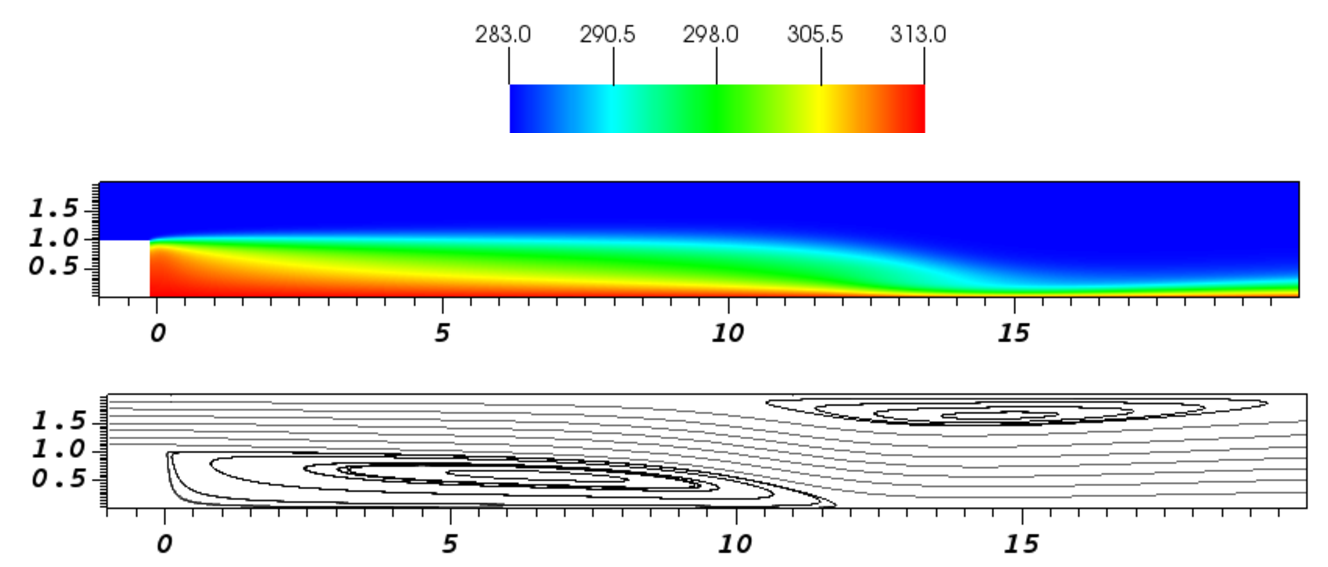
\includegraphics[width=\linewidth]{../plots/HBFS_TemperatureRe700_2.pdf}
		\caption{Temperature profile (top) and streamlines (bottom) corresponding to the backward-facing Step configuration for $\gls{Reynolds} = 400$ and an expansion ratio of two.}
		\label{BFS_Streamlines}
	\end{center}	
\end{figure} 

As an extension to the previous case, we seek to reproduce the results presented by \cite{xieFluidFlowHeat2016}, where the same backward-facing step configuration as presented in \cref{ssec:BackwardFacingStep} is studied, but with the particularity that in this case the bottom wall is heated to a constant temperature higher than the inlet temperature, thus featuring a non-isothermal system. The fluid entering the system has a temperature equal to $T_0 = \SI{283}{\kelvin}$ and the bottom wall is set to a constant temperature of $T_1 =\SI{313}{\kelvin}$
In the work of \cite{xieFluidFlowHeat2016} results are reported for the local Nusselt numbers and local friction coefficients $f_d$  along the bottom wall for different expansion ratios and Reynolds numbers. By putting together the definition of the Nusselt number ( $\gls{Nusselt} = \frac{\gls{HeatTransCoef}\hat{L}}{\gls{HeatConductivity}}$), Newtons law of cooling ($\hat{\vec{q}} = \hat{h} (\hat{T}_0 - \hat{T}_W )$), and Fourier's law of heat  conduction, ($\hat{\vec{q}} = \hat \lambda \hat{\nabla} \glsHat{temp}$) a expression for the local Nusselt number is obtained
\begin{equation}
\gls{NusseltLoc} = \frac{\hat L}{\hat T_0-\hat T_W}\hat \nabla \hat T \cdot \hat {\vec{n}}
\end{equation}
where $\hat L$ is a reference length. We choose $ \hat L = \hat S$. Additionally by recognizing that the wall shear stress along the bottom wall $\tau_{\text{w}} = -\mu \nabla u \cdot \vec{n}$, the local friction factor can be written as
\begin{equation}
f_d = \frac{8\nu} { (U_{\text{mean}})^2}  \nabla u \cdot \vec{n} 
\end{equation}
It should be noted that, for the range of temperature differences involved in this case, the variation of physical parameters such as density, viscosity and thermal conductivity with respect to temperature has no appreciable influence on the calculated flow fields.

Simulations for different Reynolds numbers and expansion ratios were conducted. In \cref{BFS_Streamlines} the temperature field and streamlines corresponding to a calculation with $\gls{Reynolds} = 700$ is shown. Here the apparition of the secondary vortex is appreciated.

It must be noted here that the results obtained by us are substantially different from those reported by \cite{xieFluidFlowHeat2016}, and will not be shown here. However, in the work of \cite{henninkLowMachNumberFlow2022} the same is also pointed out, saying that with his method it was not possible to reproduce the results presented by \cite{xieFluidFlowHeat2016}. Comparing our results with those of Hennink we can observe that the same results are obtained. as demonstrated in \cref{fig:fd_Nu_plot}. We can conclude from these results that the solver is able to deal with non-isothermal flows adequately.  

\begin{figure}[tb]
	\pgfplotsset{
		group/xticklabels at=edge bottom,
		legend style = {
			at ={ (0.59,1.0), anchor= north east}
		},
		unit code/.code={\si{#1}}
	}
\inputtikz{fd_Nu_plot1}
\inputtikz{fd_Nu_plot2}
	\caption{Local friction factor and local Nusselt number along the bottom wall for $\gls{Reynolds} = 700$ and an expansion ratio of two. The solid lines corresponds to our solution and the marks to the reference \citep{henninkLowMachNumberFlow2022}}
	\label{fig:fd_Nu_plot}
\end{figure}



\FloatBarrier

\subsection{Couette flow with vertical temperature gradient} \label{ssec:CouetteFlowTempDiff}
\begin{figure}[tb]
	\begin{center}
		\def\svgwidth{0.5\textwidth}
		\import{./plots}{HeatedCouetteSketch.pdf_tex}
		\caption{Schematic representation of the couette flow with temperature difference test case.}
		\label{fig:CouetteTempDiff_scheme}
	\end{center}	
\end{figure} 
As a following test case for the low-Mach solver we study a Couette-flow with a vertical temperature gradient. This configuration was already studied in \citep{kleinHighorderDiscontinuousGalerkin2016}, where the SIMPLE algorithm in a DG framework was used. We intend in this section to reproduce their results by using our fully coupled solver. Additionally, we show how our implemented solver performs in relation to the SIMPLE based solver. 

In \cref{fig:CouetteTempDiff_scheme} a schematic representation of the test-case is shown. The top wall corresponds to a moving wall ($u = 1$) with a fixed temperature $T=T_h$. The bottom wall is a static one ($u = 0$), and has a constant temperature $T = T_c$. 
The domain is chosen as $\Omega = [0,1]\times[0,1]$, and Dirichlet boundary conditions are used for all boundaries. Additionally,the system is subjected to a gravitational field, where the gravity vector only has a component in the $y$ direction. Under this conditions, the x-component of velocity, pressure and temperature are only dependent on the $y$ coordinate, i.e. $u = u(y)$, $T = T(y)$ and $p = p(y)$. %Thus, the governing equations (\cref{eq:NS-eq}) reduce to 
\begin{align}
&\frac{1}{\gls{Reynolds}} \pfrac{ }{y}\left(\mu\pfrac{u}{y}\right) = 0,\\
&\pfrac{p}{y} = -\frac{\gls{dens}}{\gls{Froude}^2},\\
&\frac{1}{\gls{Reynolds}~\gls{Prandtl}} \pfrac{ }{y}\left(\gls{HeatConductivity}\pfrac{T}{y}\right) = 0.
\end{align}
It is possible to find an analytical solution for this problem.
%%Constant transport properties
%By assuming $\gls{Prandtl} = 1.0$ and constant transport properties ($\mu = \lambda = 1$), we can derive the analytical solution of XXX
%\begin{align}
%u &= y,\\
%p &= - \frac{p0}{\gls{Froude}^2(T_h-T_c)}\ln\left((T_h-T_c)y+T_c\right)+C,\\
%T &= (T_h-T_c)y + T_c,
%\end{align}
%where $C$ is an arbitrary constant which defines the mean value of the pressure TODO rewritethis.
% Variable transport properties
Under this conditions, and by assuming a temperature dependence of the transport properties according to a Power Law ($\mu = \lambda = T^{2/3}$) a solution is obtained as 
\begin{subequations}
\begin{align}
	u(y) &= C_1 + C_2\left(y + \frac{T_c^{5/3}}{T_h^{5/3}-T_c^{5/3}} \right)^{3/5},\label{eq:CouetteU}\\
	p(y) &= -\frac{5p_0}{2\gls{Froude}^2}\frac{\left(y\left(T_h^{5/3}-T_c^{5/3}\right)+T_c^{5/3}\right)^{2/5}}{\left(T_h^{5/3}-T_c^{5/3}\right)}+C,\label{eq:Couettep}\\
	T(y) &= \left(C_3 - \frac{5}{3}C_4 y\right)^{3/5}\label{eq:CouetteT}.
\end{align} 
\end{subequations}
Where the constants $C_1$, $C_2$, $C_3$ and $C_4$ are determined by using the boundary conditions on the top and bottom walls, and are given by 
\begin{align}
C_1 &= \frac{\left(\frac{T_c^{5/3}}{T_h^{5/3}-T_c^{5/3}}\right)^{3/5}}{\left(\frac{T_c^{5/3}}{T_h^{5/3}-T_c^{5/3}}\right)^{3/5}-\left(\frac{T_h^{5/3}}{T_h^{5/3}-T_c^{5/3}}\right)^{3/5}}\\
C_2 &= \frac{1}{\left(\frac{T_h^{5/3}}{T_h^{5/3}-T_c^{5/3}}\right)^{3/5}-\left(\frac{T_c^{5/3}}{T_h^{5/3}-T_c^{5/3}}\right)^{3/5}}\\
C_3 &= T_c^{5/3},\\
C_4 &= \frac{3}{5}\left(T_c^{5/3}-T_h^{5/3}\right)
\end{align}
and $C$ is a real-valued arbitrary constant for the pressure.%
\begin{center}
\begin{figure}[tb]
	\pgfplotsset{
		group/xticklabels at=edge bottom,
	}
\inputtikz{CouetteSolution1}
\inputtikz{CouetteSolution2}
\inputtikz{CouetteSolution3}
	\caption{Solution of the Couette flow with vertical temperature gradient. Viscosity and heat conductivity are calculated with a Power-Law.}
	\label{fig:CouetteSolution}
\end{figure}
\end{center}
\FloatBarrier
For all calculations of this configuration shown the dimensionless parameters are set as $\gls{Reynolds} = 10$ and $\gls{Prandtl} =0.71$, $T_h = 1.6$ and $T_c = 0.4$. Since we are dealing with an open system we set $p_0 =1.0$. The Froude number is calculated as 
\begin{equation}
\text{Fr} = \left( \frac{2\text{Pr}(T_h-T_c)}{(T_h+T_c)}\right)^{1/2}
\end{equation}
In \cref{fig:CouetteSolution} the solution for the velocity, pressure and temperature are shown. The results are for a mesh with $26\times26$ elements and a polynomial degree of three for $u$ and $T$, and a polynomial degree of two for $p$.
\subsubsection{h-convergence study}
The convergence properties of the DG method for this non-isothermal system was studied using the analytical solution described before. The domain is discretized and solved in uniform Cartesian meshes with $16\times16$, $32\times32$, $64\times64$ and $128\times128$ elements. The polynomial degrees for the velocity and temperature are changed from 1 to 4 and for the pressure from 0 to 3. The convergence criteria described in \cref{ssec:TerminationCriterion} was used for all calculations. The  analytical solution given by \cref{eq:CouetteU,eq:Couettep,eq:CouetteT} are used as Dirichlet boundary conditions on all boundaries of the domain. The error is calculated against the analytical solution using the $L^2$ norm. %TODO \todo[inline]{Comment more on the calculation of the l2norm}.
In \cref{fig:ConvergenceDHC} the results of the h-convergence study are shown. We observe how the expected convergence rates are reached for all variables, namely a slope of the order $k+1$ for both velocity components and the temperature, and a slope of $k'+1$ for the pressure.
\begin{figure}[t!]
	\centering
	\pgfplotsset{width=0.34\textwidth, compat=1.3}
	\inputtikz{ConvergenceCFTD}
	\caption{Convergence study of the Couette-flow with temperature difference. A power-law is used for the transport parameters.}\label{fig:ConvergenceCFTD}
\end{figure}

\subsubsection{Comparison with SIMPLE}
As mentioned before, a solver for solving low-Mach flows based on the SIMPLE algorithm (presented in \cite{kleinHighorderDiscontinuousGalerkin2016}) has been already developed and implemented within the BoSSS framework. 
Though the solver was validated and shown to be useful for a wide variety of test cases, there were also disadvantages inherently associated with the SIMPLE algorithm. Within the solution algorithm, Picard-type iterations are used to search for a solution. This requires some prior knowledge from the user in order to select suitable relaxation factor values that provide stability to the algorithm, but at the same time do not slow down the computation substantially.
It was also observed that the calculation times were prohibitively high for some test cases. This point motivated the development of the solver presented in the present work, where the system is solved in a monolytic way and  and the Newton method globalized with a Dogleg-type method is used to solve the system.  
%TODO \todo[inline]{what are exactly the advantages of the present solver? multigrid? Ortogonalization?} 
We intend to show in this section a comparison of runtimes of the calculation of the Couette flow with vertical temperature gradient between the DG-SIMPLE algorithm \citep{kleinHighorderDiscontinuousGalerkin2016} and the present solver (denoted here as XNSEC). Calculations were performed on uniform Cartesian meshes with $16\times16$, $32\times32$, $64\times64$ and $128\times128$ elements, and with varying polynomial degrees between 1 and 3 for the velocity and temperature, and between 0 y 2 for the pressure. All calculations where initialized with a zero velocity and pressure field, and with a temperature equal to one in the whole domain. Are calculations were performed single-core and the convergence criteria is set to $10^{-8}$ for both solvers. The under-relaxation factors for the SIMPLE algorithm were set for all calculations to 0.8, 0.5 and 1.0 for the velocity, pressure and temperature, respectively. 

In figure \cref{fig:RuntimeComparison} a comparison of the runtimes from both solvers is shown. It is clearly  appreciated how the runtimes of the SIMPLE algorithm are higher for almost all of the cases studied. Obviously the under-relaxation parameters of the SIMPLE algorithm have an influence on the calculation times and an appropiate selection of them could decrease the runtimes. This is a clear disadvantage, because the selection of adequate factors is highly problem dependent and requires some previous expertise from the user. On the other hand, the globalized Newton method used by the XNSEC avoid this problem by using a more sophisticated method and heuristics in order to find a better path to the solution. 

%TODO \todo[inline]{I have to somehow highlight even more the positive points of using this solver} 

\begin{center}
	\begin{table}[tb!]
		\begin{tabular}{ccc}
			\inputtikz{RuntimeComparison1}
			&
			\inputtikz{RuntimeComparison2}
			&
					\inputtikz{RuntimeComparison3}
		\end{tabular}%
		\caption{Runtime comparison of the DG-SIMPLE algorithm \citep{kleinHighorderDiscontinuousGalerkin2016} and the present solver (XNSEC) for the Couette flow with vertical temperature gradient configuration}
		\label{fig:RuntimeComparison}
	\end{table}
\end{center} 


\FloatBarrier



\subsection{Differentially heated cavity problem}\label{ss:DHC}

\begin{figure}[bt]
	\begin{center}
		\def\svgwidth{0.53\textwidth}
		\import{./plots/}{diffheatedCavityGeometry.pdf_tex}		
	\caption{Schematic representation of the differentially heated cavity problem.}
		\label{DHCGeom}
	\end{center}	
\end{figure} 



The differentially heated cavity problem corresponds to a classical benchmark case often used to asses the capability of numerical codes to simulate variable density flows. \cite{paillereComparisonLowMach2000,vierendeelsBenchmarkSolutionsNatural2003,tyliszczakProjectionMethodHighorder2014} In this section, we show the basic set-up and compare our results with the ones presented in the work of Vierendeels et al. \cite{vierendeelsBenchmarkSolutionsNatural2003} where benchmark solutions for the differentially heated cavity are presented. They solve the fully compressible Navier-Stokes equations on a $1024\times1024$ stretched grid using a Finite Volume Method with quadratic convergence.

The differentially heated cavity problem consists of a two-dimensional fully enclosed square cavity filled with fluid.  A sketch of the problem is shown in \cref{DHCGeom}. The left and right walls of the cavity have a constant temperature $\hat{T}_h$ and $\hat{T}_c$ respectively, with $\hat{T}_h >\hat{T}_c$, and the top and bottom walls are adiabatic. A gravity field induces fluid movement due to the density differences caused by the difference of temperature between the hot and cold walls.

The natural convection phenomenon is characterized by the Rayleigh number, defined as 
\begin{equation}\label{eq:Rayleigh}
\text{Ra} = \Prandtl \frac{\hat g \RefVal{\rho}^2(\hat T_h-\hat T_c) \RefVal{L}^3}{\RefVal{T}\RefVal{\mu}^2},
\end{equation}
For small values of $\text{Ra}$, conduction dominates the heat transfer process, and a boundary layer covers the whole domain. On the other hand large values of $\text{Ra}$ represent a convection dominated flow. For increasing $\text{Ra}$ number, a thinner boundary layer is formed. 

\paragraph{Set-up}
A reference velocity for buoyancy driven flows can be defined as\cite{vierendeelsBenchmarkSolutionsNatural2003}
\begin{equation}
\RefVal{u} = \frac{\sqrt{\text{Ra}} \RefVal{\mu}}{\RefVal{\rho}\RefVal{L}}.
\end{equation} 
The Rayleigh number is then related to the Reynolds number according to
\begin{equation}
\text{Re} = \sqrt{\text{Ra}}.
\end{equation}
Thus it is sufficient to select a $\Reynolds$ number in our simulation, fixing the value of the $\text{Ra}$ number. The driving temperature difference $(\hat T_h - \hat T_c)$ appearing in \cref{eq:Rayleigh} can be represented as an non-dimensional parameter:
\begin{equation}\label{eq:nondimensionalTemperature}
\varepsilon = \frac{\hat T_h - \hat T_c}{2\RefVal{T}}.
\end{equation}
Using these definitions, the Froude number can be calculated as 
\begin{equation}
\Froude = \sqrt{\Prandtl 2 \varepsilon}.
\end{equation}
All calculations assume a constant Prandtl number equal to 0.71. The viscosity and heat conductivity  dependence on temperature is calculated using \cref{eq:nondim_sutherland}.
Our results are calculated and compared with those of the reference solution for $\RefVal{T} = 600\si{K}$  and $\varepsilon = 0.6$. The non-dimensional length of the cavity is $L=1$. The non-dimensional temperatures $T_h$ and $T_c$ are set to 1.6 and 0.4, respectively. 
Since the cavity contains a single species, it is governed by the equations for continuity, momentum and temperature (\crefrange{eq:LowMachConti}{eq:LowMachEnergy}) and no equation for species transport is needed. Thus $n_s = 1$ and  $Y_1 = 1$ in the whole domain.  Moreover, the non-dimensional equation of state (\cref{eq:ideal_gas}) only depends on the temperature and reduces to
\begin{equation}
\rho = \frac{p_0}{T}.
\end{equation}
The thermodynamic pressure $p_0$ in a closed system and has to be adapted in order to ensure mass conservation. If $m_0$ is the initial total mass of the system, the thermodynamic pressure is given by
\begin{equation}
p_0 = \frac{m_0}{\int_\Omega \frac{1}{T}\text{d}V}, \label{eq:p0Condition}
\end{equation}
where $\Omega$ represents the complete closed domain. The initial mass of the system $m_0$ is constant and we set $m_0 = 1.0$. Within the solution algorithm, \cref{eq:p0Condition} is used to update the value of the thermodynamic pressure after each Newton-Dogleg iteration.
Moreover, the benchmark solution \cite{vierendeelsBenchmarkSolutionsNatural2003} also reports the Nusselt number and thermodynamic pressure associated with a given Rayleigh number. The Nusselt number is defined for a given wall $\Gamma$ in its averaged form as 
\begin{equation}\label{eq:Nusselt}
\text{Nu}_\Gamma = \frac{1}{T_h - T_c}\int_{\Gamma} k \pfrac{T}{x}\text{d}y.
\end{equation}\begin{table}[t]
	\begin{center}
		\begin{tabular}{cccccc}
			\hline
			Rayleigh & $p_0$ &  $p_{0,\text{ref}}$  &$\text{Nu}_{h}$ & $\text{Nu}_{c}$& $\text{Nu}_{\text{ref}}$ \\ \hline
			\parbox[0pt][13pt][c]{0pt}{}$10^2$   & 0.9574 & 0.9573 & 0.9787    & 0.9787 & 0.9787      \\
			$10^3$   & 0.9381 & 0.9381 & 1.1077    & 1.1077  & 1.1077      \\
			$10^4$   & 0.9146 & 0.9146 & 2.2180    & 2.2174  & 2.2180      \\
			$10^5$   & 0.9220 & 0.9220 & 4.4801    & 4.4796   & 4.4800      \\
			$10^6$   & 0.9245 & 0.9245 & 8.6866    & 8.6791  & 8.6870      \\
			$10^7$   & 0.9225 & 0.9226 & 16.2411   & 16.1700 & 16.2400     \\ \hline
		\end{tabular}
	\end{center}
	\caption[Differentially heated cavity: Results of Nusselt number and Thermodynamic pressure]{Comparison of calculated Nusselt numbers of the hot and cold wall and Thermodynamic pressure $p_0$ reported values\cite{vierendeelsBenchmarkSolutionsNatural2003} for the differentially heated cavity. Results are obtained for polynomial degree of four for the velocities and temperature, three for the pressure in an equidistant $128x128$ mesh.}
	\label{tab:p0_Nu_Results}
\end{table}
\paragraph{Comparison of results with benchmark solution}
The benchmark results \cite{vierendeelsBenchmarkSolutionsNatural2003} are presented for $\text{Ra} = \{10^2,10^3,10^4,10^5,10^6,10^7\}$. In this range of Rayleigh numbers the problem has a steady-state solution, thus we are able to use our steady formulation of the problem. The cavity is represented by the domain $[0,1]\times[0,1]$. We use an equidistant Cartesian mesh with $30 \times 30$ elements for each simulation. A polynomial degree of five is used for the velocities and temperature, and a degree of four for the pressure. 
It is observed that for cases until  $\text{Ra} = 10^5$ the solution of the system using Newton's method is possible without further modifications, while for higher values the algorithm diverges. The homotopy strategy mentioned in \cref{sec:CompMethodology} is used to overcome this problem and obtain solutions for higher Rayleigh (and equivalently higher Reynolds) numbers. Here, the Reynolds number is selected as the homotopy parameter and continuously increased until the desired value is reached.
In \cref{fig:TempProfile,fig:VelocityXProfile,fig:VelocityYProfile} temperature and velocity profiles for different Rayleigh numbers are shown. The profiles calculated with \BoSSS agree closely to the benchmark solution. As expected we observe 
an increase of the acceleration of the fluid in the vicinity of the walls for increasing Rayleigh numbers, forming a thin boundary layer. 



\begin{figure}
	\centering
	\pgfplotsset{width=0.45 \textwidth, compat=1.3}
	\inputtikz{HSCStreamlines}
	\caption{Streamlines of the heated cavity configuration with $\epsilon = 0.6$.}\label{fig:HSCStreamlines}
\end{figure}


\begin{figure}[!htb]
	\centering
	\pgfplotsset{width=0.20\textwidth, compat=1.3}
	\inputtikz{VelocityXProfile}
	\caption{ Profiles of the x-velocity component along the vertical line $x=0.5$. Solid lines represents our solution and the marks the benchmark solution. \cite{vierendeelsBenchmarkSolutionsNatural2003}}
	\label{fig:VelocityXProfile}
\end{figure}


\begin{figure}[b!]
	\centering
	\pgfplotsset{width=0.20\textwidth, compat=1.3}
	\inputtikz{VelocityYProfile}
	\caption{ Profiles of the y-velocity component along the horizontal line $y=0.5$. Solid lines represents our solution and marks the benchmark solution. \cite{vierendeelsBenchmarkSolutionsNatural2003}}
	\label{fig:VelocityYProfile}
\end{figure}

We also compare the thermodynamic pressure and the Nusselt numbers to the benchmark solution. The results are shown in \cref{tab:p0_Nu_Results}. The thermodynamic pressure is obtained from \cref{eq:p0Condition}, and the Nusselt number is calculated with \cref{eq:Nusselt}. We observe that our results are in very good agreement with the reference results, and the thermodynamic pressure differ at most in the fourth decimal place. Note that the Nusselt number of the heated  wall $(\text{Nu}_\text{h})$ and the Nusselt number of the cold wall $(\text{Nu}_\text{c})$ are different.  As the Rayleigh number grows, this discrepancy becomes bigger, hinting that at such Rayleigh numbers the used mesh is not refined enough  to represent adequately the thin boundary layer and more complex flow structures appearing at high-Rayleigh cases. While for an energy conservative system $\text{Nu}_\text{h}$ and $\text{Nu}_c$ should be equal, for our formulation this is not the case and the values differ slightly. This discrepancy can be seen as a measure of the discretization error from the DG formulation.\cite{kleinHighorderDiscontinuousGalerkin2016} This hints that the discrepancy between Nusselt numbers should decrease when increasing the mesh resolution, which will be discussed in the next section. 

\begin{figure}[b!]
	\centering
	\pgfplotsset{width=0.20\textwidth, compat=1.3}
	\inputtikz{TempProfile}
	\caption{Temperature profiles for the differentially heated square cavity along different vertical levels. Solid lines represent our solution and marks the benchmark solution. \cite{vierendeelsBenchmarkSolutionsNatural2003}}
	\label{fig:TempProfile}
\end{figure}

\begin{figure}[b!]
	\centering
	\inputtikz{NusseltStudy}
	\caption{Nusselt numbers calculated with \cref{eq:Nusselt} at the hot wall ($\text{Nu}_h$) and the cold wall ($\text{Nu}_c$) for different number of cells and polynomial order $k$. The reference values\cite{vierendeelsBenchmarkSolutionsNatural2003} are shown with dashed lines.}\label{fig:NusseltStudy}
\end{figure}

\paragraph{Convergence study}\label{ssec:ConvStudyHeatedCavity}
An $h-$convergence study of the differentially heated cavity configuration was conducted. Calculations were done for polynomial degrees $k = {1,2,3,4}$ and equidistant regular meshes with respectively $8, 16, 32, 64, 128$ and $256$ elements in each spatial coordinate.  The $L^2$-Norm was used for the calculation of the errors against the solution on the finest mesh. Results of the $h$-convergence study for varying polynomial orders $k$ are shown in \cref{fig:ConvergenceDHC}. Recall that for increasing polynomial order, the expected order of convergence is given by the slope of the line curve when cell length and errors are presented in a log-log plot. Because we are using a mixed order formulation the slopes should be equal to $k$ for the pressure and equal to $k+1$ for all other variables.  It is observed how convergence rates scale approximately as $k+1$. Interestingly, for $k=2$ the rates are higher than expected. On the other hand, some degeneration on the convergence rates is observed for $k = 4$.

As discussed in the last section, the difference on values of the Nusselt number on the hot wall $\text{Nu}_\text{h}$ and the cold wall $\text{Nu}_c$ is a consequence of spatial discretization error. In \cref{fig:NusseltStudy} the convergence behaviour of the Nusselt number for different polynomial degrees $k$, different number of elements and for two different Ra numbers is presented. As expected, it can be observed that this discrepancy is smaller when a higher number of elements is used. 


\begin{figure}[t!]
	\centering
	\pgfplotsset{width=0.34\textwidth, compat=1.3}
	\inputtikz{ConvergenceDHC}
	\caption{Convergence study of the differentially heated cavity problem for $\text{Ra} = 10^3$.}\label{fig:ConvergenceDHC}
\end{figure}




\subsection{Poiseuille–Rayleigh–Bénard instability in a channel}
\blindtext[5]


\subsection{Flow around a heated cylinder}
\subsubsection{Square cylinder}
\blindtext[5]
\subsubsection{Circle? cylinder}
\blindtext[5]



\section{Multi-component non-isothermal cases}\label{sec:MultCompNonIsothermCase}
Later in in \cref{ss:CDF} and \cref{ss:CoFlowFlame} two different configurations for reactive flows are presented. 
In the following, we show results of the simulations of two test cases with combustion, namely the counterflow diffusion flame and the chambered diffusion flame. For both cases, the solution of the flame sheet problem described in \cref{ssec:FlameSheet} is calculated first. This solution is used subsequently as initial estimates for the solution of the finite chemistry rate problem (c.f. \cref{ssec:NonDimLowMachEquations}). In all test cases presented in this section, a smoothing parameter $\sigma = 50$ was used (c.f. \cref{ssec:FlameSheet}). For all test cases methane combustion according to the one-step model shown in \cref{sec:ChemModel} is considered. The mass fraction transport \cref{eq:LowMachMassBalance} is solved for the species \ch{CH4}, \ch{O2}, \ch{CO2} and \ch{H2O}, thus $\vec{Y}' = \left(Y_{\ch{CH4}},Y_{\ch{O2}},Y_{\ch{CO2}},Y_{\ch{H2O}}\right)$. The nitrogen mass fraction $Y_{\ch{N2}}$ is calculated according to \cref{eq:MassFractionConstraint}. 



\subsection{CoFlowing flame?}

As a first test for assessing basic behaviour related to combustion, a cofloing flame configuration used. This test case is the main prototype flame for diffusion regimes \cite{poinsotTheoreticalNumericalCombustion2005}. It is set up by sending a stream of fuel against a stream containing oxidizer. A diagram can be seen in X
%TODO ACA VA UN sketch del coflowing flame con las boundary conditions 
\begin{figure}[t!]
	\centering
	\pgfplotsset{
		compat=1.3,
		tick align = outside,
		yticklabel style={/pgf/number format/fixed}, 
	}
	\inputtikz{CoFlow_ConvergenceStory}
	\caption{Typical convergence history of a diffusion flame in the coflowing flame configuration with mesh refinement.}
	\label{fig:CoFlow_ConvergenceStory}
\end{figure} 
% \begin{figure}[t!]
% 	\begin{center}
% 		\def\svgwidth{0.5\textwidth}

% 		\caption{Schematic representation of strained diffusion flame}
% 		\label{SSDFSketch}
% 	\end{center}	
% \end{figure}
The area where the chemical reaction takes place is usually a thin region, which thickness is defined by the availability of reactants, which at the same time are controled by the velocity which the chemical reaction happens. This factor is governed by the $Da$ number in the non-dimensional formulation (sure??). It is of critical importance for the numerical simulation that the flame is resolved accordingly, which can demand a very fine mesh. Not doing so can provoke non-physically effects to occur, as for example negative values of the reaction term $\omega$ (in the present formulation the reaction is irreversible, and thus only positive values of $\omega$ make sense). 

For avoiding over-resolving in zones where actually no reaction is taking place (or very slowly), an adaptive mesh refinement strategy  (see section X) within a pseudo-time-stepping framework was used.  Here a  suitable strategy for choosing cells to be refined is necesary . For reactive flows, this strategy is based on the variable $\omega$.
Before each refinement step the values of $\omega$ are normalized by the biggest value of the domain, and according to this normalized effects the cells are refined. %In Figure \ref{fig:AMR} the refined meshes can be seen. The legend of the pseudocolor plots is not shown, because for each plot the magnitude scales are different, and just the normalized value accounts for the AMR. 


\begin{figure}
	\centering
	\pgfplotsset{width=0.75 \textwidth, compat=1.3}
	\inputtikz{CoFlowFlameFig1}
	\inputtikz{CoFlowFlameFig2}	
	\caption{Coflowing Flame.} \label{fig:CoFlowFlameFig}
\end{figure}
\subsection{Counterflow diffusion flame}\label{ss:CDF}	

\begin{figure}[b]
	\begin{center}
		\def\svgwidth{0.8\textwidth}
		\import{./plots/}{CounterDiffusionFlame_sketch_rotated2.pdf_tex}		
\caption{Schematic representation of the counterflow configuration.}
\label{fig:CDFScheme}
	\end{center}	
\end{figure} 

The counterflow diffusion flame is a canonical configuration used to study the structure of non-premixed flames. In its most basic configuration it consists of two oppositely situated jets. The fuel (possibly mixed with some inert component such as nitrogen) is fed into the system by one of the jets, while the other jet feeds air to the system, thereby establishing a stagnation point flow. Upon contact, the reactants produce a flame which is located in the vicinity of the stagnation plane. A diagram of the setup can be seen in \cref{fig:CDFScheme}. This simple configuration has been subject of study for decades  because it provides a simple way of creating a strained diffusion flame, which proves to be useful when studying the flame structure, extinction limits or production of pollutants of flames \cite{pandyaStructureFlatCounterFlow1964} \cite{spaldingTheoryMixingChemical1961} \cite{keyesFlameSheetStarting1987}. By assuming an infinite injector diameter and self-similarity of the solution, it is possible to reduce the governing equations to a one-dimensional formulation (see e.g. the textbook of Kee \cite{keeChemicallyReactingFlow2003}). As a means of validating our implementation we compare the results with the solution of the one-dimensional self-similar problem calculated with \lstinline|BVP4|, a fourth order finite difference boundary value problem solver provided by \lstinline|MATLAB|. 

The combustion of a methane-nitrogen mixture with air was simulated using the \BoSSS code. The mass composition of the fuel inlet was assumed to be  $Y^0_{\ch{CH4}} = 0.2$ and $Y^0_{\ch{N2}} = 0.8$, and the oxidizer inlet corresponds to air with   $Y^0_{\ch{O2}} = 0.23$ and $Y^0_{\ch{N2}} = 0.77$. Because we are dealing with an open system, the thermodynamic pressure $\hat p_0$ is constant and set to the ambient pressure of $\SI{101325}{\pascal}$. As noted by Sung et al., \cite{sungStructuralResponseCounterflow1995} although the form of the inlet velocity profiles does have an influence on the solution of the problem, its effect on the solution near the flame zone is rather small. Nevertheless, as mentioned before the solution of the self-similar one-dimensional problem assumed an infinite injector diameter, which implies that the upstream velocity field has to be constant. Based on this fact we set the velocity profile of both inlets as a plug flow. Following combinations of inlet velocities were calculated:
\begin{itemize}
	\item  Low inlet velocities:  $u^0_{\text{fuel}} = \SI{0.048}{\meter \per \second}$ and  $u^0_{\text{oxidizer}} = \SI{0.144}{\meter \per \second}$,
	\item Medium inlet velocities:  $u^0_{\text{fuel}} = \SI{0.12}{\meter \per \second}$ and  $u^0_{\text{oxidizer}} = \SI{0.36}{\meter \per \second}$
	\item High inlet velocities: $u^0_{\text{fuel}}  = \SI{0.24}{\meter \per \second}$ and   $u^0_{\text{oxidizer}} = \SI{0.72}{\meter \per \second}$
\end{itemize}
By using as definition of the strain rate the maximum axial velocity gradient, the calculated strains for the three cases mentioned above are $\SI{34}{\per\second}$, $\SI{76}{\per\second}$ and $\SI{155}{\per\second}$, respectively. The temperature of both inlets is \SI{300}{\kelvin}. The separation between both jets $\hat L$ is equal to $\SI{0.02}{\meter}$, and the length of the inlet opening $\hat D$ is $\SI{0.02}{\meter}$. The left and right domain boundaries are selected to be at a distance $3\hat L$ of the center. A non-unity but constant Lewis number formulation is used,with  
$\Lewis_{\ch{CH4}} =  0.97 $ , $\Lewis_{\ch{O2}} = 1.11 $, $\Lewis_{\ch{H2O}} = 0.83 $ and $\Lewis_{\ch{CO2}} = 1.39 $.\cite{smookePremixedNonpremixedTest1991} The heat capacity of each component is evaluated locally from NASA polynomials, and the mixture heat capacity is calculated with \cref{eq:nondim_cpmixture}.
%\tikzset{external/export next=false}
\begin{figure}[t!]
	\centering
	\pgfplotsset{
		compat=1.3,
		tick align = outside,
		yticklabel style={/pgf/number format/fixed}, 
	}
\inputtikz{CDF_ConvergenceStory}
	\caption{Convergence history of the diffusion flame in the counterflow configuration, with a maximum strain value of $165.1 $\si{s^{-1}}}
	\label{fig:CDF_ConvergenceStory}
\end{figure} 

In \cref{fig:CDF_ConvergenceStory} the convergence history obtained for a typical calculation of the counter diffusion flame is presented. The solution of the flame sheet calculation requires 17 iterations until convergence is reached. The obtained solution is used as a starting value for the finite chemical rate calculation, which only needs 10 iterations until convergence is reached. We note that because the flame sheet calculation is only used as an approximation of the final solution, a low polynomial degree can be used. For the flame sheet calculation $k = 2$ was chosen, resulting in a rather small system with 26,880 degrees of freedom. For the finite rate calculation $k = 4$ was used, which resulted in a system with 174,110 degrees of freedom.  With the above-mentioned another advantage of the approach of using the flame sheet calculation for two-dimensional simulations can be highlighted. The initial estimate can be found relatively easily for a system with few degrees of freedom. Using the solution found as the initial estimate has the consequence that Newton's algorithm for the complete problem (which has many more degrees of freedom) only needs a few iterations to find a solution. 

Because we are solving a two-dimensional configuration, in order to be able to compare our results with the ones obtained from the one-dimensional representation, the temperature, mass fractions and velocity profiles are extracted along the centerline of the system shown as the dashed line in \cref{fig:CDFScheme}. In \cref{fig:BoSSS_1D_Comparison_velocity} a comparison of the axial velocities calculated with \BoSSS and the one-dimensional solution is shown. While for the high strain case the results agree closely, for lower strains a discrepancy is observed. Recall that the derivation of the one-dimensional approximation assumes a constant velocity field incoming to the flame zone in order to obtain a self-similar solution. In the case of the two-dimensional configuration presented here, the border effects do have an influence on the centerline, which disrupts the self-similarity. This effect is more pronounced for low velocities, which explains the discrepancy between curves. Similarly, In \cref{fig:BoSSS_1D_Comparison} the temperature and mass fraction fields are presented. Again, a discrepancy is observed for low strains, but results show a good agreement for higher inlet velocities. It can also be observed how, as expected, \cite{fernandez-tarrazoSimpleOnestepChemistry2006} at higher strains a significant penetration (leakage) of oxygen across the flame is present. Finally, in \cref{fig:TempAndReacFields} the two-dimensional temperature, velocity and reaction rate fields for the case (a) are shown. 

Finally, in \Cref{fig:TemperatureConvergenceDiffFlame} we show how the maximum value of the temperature behaves for different mesh resolutions and polynomial degrees. The temperature tends to a limit value, and we observe how this value is reached already for coarse meshes when using a polynomial degree of three or four. We also observe that for $k=2$ the temperature tends to a limit value, but slower in comparison to $k =3$ or $4$. The values for $k=1$ are not displayed because for the mesh resolutions shown here, the values of the maximum temperature were of the order of 50 \si{K} bigger than the limit value. We note that the solution of this configuration showed singularities in the boundary points where the inlet and wall meet. This fact made hard to realize a $h$-convergence study for the complete domain. Based on this we decided to analyse a flame configuration that doesn't exhibit this behaviour, as shown in the next section.


We note that the solution of this configuration showed singularities in the boundary points where the inlet and wall meet, which induces a pollution phenomenon on the accuracy of the solution. This fact made hard to realize an $h$-convergence study for the complete domain. Based on this fact we decided to analyze a flame configuration that does not exhibit this behaviour, as shown in the next section.
\begin{figure}[t!]
	\pgfplotsset{
		group/xticklabels at=edge bottom,
		legend style = {
			at ={ (0.5,1), anchor= north east}
		},
		unit code/.code={\si{#1}}
	}
	\centering
	\inputtikz{BoSSS_1D_Comparison_velocity}
	\caption{ Comparison of the axial velocity calculated with \BoSSS and the one-dimensional approximation. }
	\label{fig:BoSSS_1D_Comparison_velocity}
\end{figure}
\newpage
\tikzexternaldisable
%\tikzset{external/export next=false}%%%%%%%%%%%%%%%%%%%%%%%%%%%%%%%%%%%%%%%%%%%%%%%%%%%%%%%%%%%%%%%%%%%%%%%%%%%%%%%%%%%%%%%%%%%%%%%%%%%%%%%
\begin{figure}[b!]
	\centering
	\pgfplotsset{
		width=0.85\textwidth,
		height = 0.3\textwidth,
		compat=1.3,
		tick align = outside,
		yticklabel style={/pgf/number format/fixed}, 
	}	
	\inputtikz{BoSSS_1D_Comparison1}
	\inputtikz{BoSSS_1D_Comparison2}
	\inputtikz{BoSSS_1D_Comparison3}
	\caption{Comparison of temperature and mass fraction fields obtained with \BoSSS and the one-dimensional approximation.}
	\label{fig:BoSSS_1D_Comparison}
\end{figure}
\tikzexternalenable
\newpage
\begin{figure}[b]
	\begin{center}
		\def\svgwidth{0.8\textwidth}
		\import{./plots/}{CDF_Results.pdf_tex}		
\caption{Calculated temperature and velocity fields (top picture) and reaction rate (second picture) of the counter diffusion flame configuration, case (a). The unit of the temperature is \si{K} and of the reaction rate \si{\kilo\mole \per \meter \cubed \per \second}. }
	\label{fig:TempAndReacFields}
	\end{center}	
\end{figure} 

\begin{figure}[tbp]
	\centering
	\inputtikz{TemperatureConvergenceDiffFlame}
	\caption{Maximum value of the temperature for the counter diffusion flame configuration, for different mesh sizes in the x-direction and polynomial degrees. Values for $k=1$ are not shown, because for this range of cell lengths the maximum temperature value was of the order of 50K higher than the ones depicted here.}
	\label{fig:TemperatureConvergenceDiffFlame}
\end{figure}
\FloatBarrier
\newpage
\subsection{Chambered diffusion flame}\label{ss:UDF}
\begin{figure}[b]
	\begin{center}
		\def\svgwidth{0.8\textwidth}
		\import{./plots/}{UnstrainedFlameConfig.pdf_tex}		
		\caption{Schematic representation of the chambered diffusion flame configuration. }
\label{fig:chamberedDifFlame}
	\end{center}	
\end{figure} 

The chambered diffusion flame configuration has served as a model for many theoretical studies related to diffusion flames\cite{matalonEffectThermalExpansion2010,rameauNumericalBifurcationChambered1985,matalonDiffusionFlamesChamber1980} A scheme of the configuration can be seen in \cref{fig:chamberedDifFlame}. Fuel is injected at a constant rate into the bottom of a small insulated chamber, while oxidant diffuses into the system against the direction of flow. Constant conditions at the outlet of the chamber are achieved by a rapid renewal of the flow of oxidant.  Under these conditions a planar flame forms far away from the walls, which allows a one-dimensional description of the flame structure.
The fuel inlet into the chamber is modelled with a velocity inlet boundary condition \cref{eq:bc_d}, while the flow outlet at the top is considered an outlet as given by \cref{eq:bc_OD}. Since we are interested in the flame in wall distance, it is sufficient to set the remaining boundary conditions as periodic boundaries. This effectively transforms the problem into a pseudo two-dimensional configuration. 


\begin{figure}[t!]
	\centering
	\pgfplotsset{width=0.34\textwidth, compat=1.3}
\inputtikz{ConvergenceDiffFlame}
	\caption{Convergence study for the chambered diffusion flame configuration.}
	\label{ConvergenceDiffFlame}
\end{figure}

In this test case we study the combustion of a \ch{CH4}-\ch{N2} mixture with air. The thermodynamic pressure $\hat p_0$ is set equal to an ambient pressure of $\SI{101325}{\pascal}$. The inlet velocity of the fuel jet is set to $\SI{0.025}{\meter \per \second}$ and its mass composition is $Y^0_{\ch{CH4}} = 0.2$ and $Y^0_{\ch{N2}} = 0.8$ while air has a composition $Y^0_{\ch{O2}} = 0.23$ and $Y^0_{\ch{N2}} = 0.77$. The temperature of the fuel and air feed streams is $\SI{300}{\kelvin}$. The length of the system $L$ is equal to $\SI{0.015}{\meter}$.
For this configuration an $h$-convergence study is conducted, where uniform Cartesian meshes with  $5\times2^6$, $5\times2^7$, $5\times2^8$,  $5\times2^9$ and $5\times2^{10}$  cells are used. The polynomial degrees are varied from 1 to 4 for velocity, temperature and mass fractions, and from 0 to 3 for pressure.  Errors are calculated using the finest mesh as a reference solution.  The results are shown in \cref{ConvergenceDiffFlame} for variables $u_x$, $T$, $Y_{\ch{CH4}}$ and $p$. The convergence results for other variables are similar and not shown here. We observe the expected slope increase with increasing polynomial degrees. For low polynomial degrees the orders of convergence are very close to the theoretical values. However for higher polynomial degrees we observe a slight deterioration of the convergence rate.  
\FloatBarrier
	
\cleardoublepage
\chapter{Conclusion}	\label{ch:conclusion}
%\glsresetall

In the present work the discretization and implementation of a fully coupled implicit method for simulating steady state diffusion flames using the DG-method is shown. For this the governing equations in the low-Mach limit are used, which allow to consider expansion and compression effects for large variations in temperature, not restricting to models such as the bousinesq approximation. The chemical model used corresponds to a one-step model with variable parameters that allows to capture fundamental characteristics of diffusion flames, but with the advantage that it requires much less computational power compared to complex chemical models.  Additionally, temperature dependent expressions for the transport parameters according to Sutherland's law, and variable heat capacities according to NASA-polynomials are used. The presented formulation of the equations allows the simulation of open and closed systems. 

The discretization using DG-methods allows for a high-order formulation which offers a high accuracy with low computational costs. For the DG-discretization a mixed order formulation is used for stability reasons, where velocity, temperature and mass fractions are represented by polynomials of degree $k$, and pressure by polynomials of degree $k-1$. The system obtained from the discretization is solved in a fully coupled manner by means of a Newton-Dogleg type method, which proved to be a very robust algorithm for the test cases presented, even for cases where a initial estimate was not available. Additionally, an efficient method for the calculation of the Jacobian matrix as part of the Newton's algorithm is presented. Systems of linear equations that must be solved as part of the newton algorithm are solved in two ways: Systems with up to approximately 500,000 \gls{DOFs} are solved using the direct solver \gls{PARDISO}. Larger systems are solved using a multigrid method. 

Additionally, as a convergence supporting strategy, an homotopy method is included in the structure of the non linear solver, which allows for solving highly nonlinear systems in a fully automatic manner. This type of algorithms was useful to solve steady state systems where some parameter makes difficult the solution of the system, as it is for example the simulation of the square heated cavity problem for high Rayleigh numbers. The homotopy algorithm shown here is demonstrated as a robust and automatic strategy that allows finding solutions to such problems without the need for user intervention.

For the reactive test cases the concept of the flame sheet estimate was demonstrated to be a useful and computationally cheap way of initializing steady state calculation of combustion systems with finite reaction rate. Using this strategy avoids the need for ignition simulation, which is usually performed by means of timestepping or pseudo-timestepping techniques.

Several benchmark configurations were solved with the present solver, and were shown in increasing level of complexity. First two classical incompressible benchmark cases were selected: the lid-driven cavity flow and the Backward-facing step. These cases were simulated and compared with benchmark solutions, obtaining very good agreement of the results. 

Subsequently, several testcases where the temperature plays a significant role were analysed. A heated backward-facing step was calculated and compared with benchmark results, obtaining again a very good result agreements. Later, a Couette flow configuration with a vertical temperature gradient was studied, which allowed to verify the implementation of the solver, since an analytical solution can be obtained for this problem. The analytical solution was used for determining the experimental order of convergence of the solver for single component non-isothermal systems, where the expected rates of the DG-method were observed. This test also served as a means to compare the fully implicit approach presented in this work with the SIMPLE algorithm based solver that is already present in the BoSSS framework. A clear and very large difference in the runtimes could be appreciated, where the XNSEC solver presents computation times up to 20 times shorter than the SIMPLE-DG solver. It is important to note that this is by no means an indicator that the SIMPLE-DG method is in general less efficient in terms of computational time than the approach presented in this work, since the low performance of the SIMPLE-DG method could be explained by a poor choice of under-relaxation factors. Nevertheless, the fully coupled approach presented in this work requires less user input, which makes it also more robust. Later the capability of the XNSEC solver for simulating buoyancy driven flows was tested by means of the heated square cavity problem. This testcase also served for proving the capability of solving flows in a closed system. A very thorough comparison with benchmark results was performed, obtaining very satisfactory results. The Newton-Dogleg method proved to be adequate for systems up to a Rayleigh number of $\text{Ra} = 10^5$. Larger Rayleigh number values required the use of the homotopy algorithm in order to find a converged solution. The convergence properties for the non-isothermal closed-system flow were also calculated, and the expected DG convergence rates were again obtained, only for $k=4$ a slight deterioration of the rates was observed.
Later a unsteady test case was shown, namely the flow over a heated circular cylinder. The unsteady behaviour of the solution obtained agrees very well with benchmark results, and the expected Kármán vortex street is observed. The behavior of the solver with respect to perturbations was then tested, in which the Rayleigh-Bénard convection problem was treated. The critical value of the Rayleigh number at which the system exhibits convective fluid motion was calculated with $0.009\%$ accuracy compared to theory based values. 
Finally the XNSEC solver was used for solving several classical diffusion flame configurations. First, a coflowing flame was simulated, which served to highlight the benefits of the strategy of using flame-sheet estimates, and also for showing the behaviour of the non-linear solver.
A throughout verification of the spatial discretization for the reactive case was done by means of the counterflow diffusion flame configuration. The results obtained using the XNSEC solver for this configuration at varying strain rates were compared with results obtained by using a in MATLAB implemented code for solving the equations for a quasi one-dimensional flame. Comparison of the results showed that for high strain rates the results agree very closely, while for low strain rates they differ slightly. This can be explained by the influence of the border effects on the centerline results for a two-dimensional configuration. Additionally the influence of different inlet boundary conditions types was studied, concluding that a plug flow is the most adequate for comparison with the one-dimensional equations. Finally a comparison of the maximum temperatures obtained for different strain rates showed discrepancies of up to $10\%$.
A pseudo one-dimensional flame configuration was used to study the convergence rates of the method for cases where combustion is present. And again the expected convergence rates where obtained, only observing a slight deterioration for higher polynomial orders $k$. Finally a unsteady test case was shown. It was observed that the temporal term of the continuity equation is a source of instability in cases with high temperature variations, and caused the algorithm to not converge. Nevertheless, simulations ignoring the term were performed, thus showing that the mesh refinement algorithm in a timestepping framework works as expected.

%%%%%%%%%%%%%%%%%%%%%%%%%%%%%%%%%%%%%%%%%%
\section{Future work}
% En la conclusion puedo hablar de que cosas serian necesarias en futuro trabajo
The governing equations treated in this work were based on some strong assumptions. In particular, the one-step model chemical model (esto no es tan malo).
El modelo de difusion utilizado es altamente simplificado, y se espera que en ciertos sistemas con combustion pueda arrojar resultados con un error apreciable, en particular en sistemas que no se encuentren altamente diluidos. La implementacion de un modelo de difusion más complejo, como por ejemplo la Hirschfelder and Curtiss approximation sería una forma simple y eficiente de solucionar el problema. 
En este trabajo se trató principalmente con sistemas de combustion en estado estacionario. El uso de la flame sheet solution como estimado inicial probó ser una manera eficiente de encontrar la burning solution. Con esta estrategia, se circumvent la necesidad de simular el proceso de inición de la flama puesto  que solo se está interesado en el steady state solution.  La simulación del proceso de ignicion es un topico abierto que debe ser tratado en futuros trabajos. 
Si bien en el trabajo se demostró que el fully coupled approach funcionó muy bien para una gran variedad de problemas, para sistemas más complejos, como por ejemplo procesos de combustion no estacionarios, los tiempos de calculo podrían resultar prohibitivos. Una mayor paralelización computacional, en particular de los linear-solvers, podrían brindar aceleración a los calculos. Este es un topico de actual estudio en el departamento de mecanica de fluidos FDY, en donde distintos metodos para resolucion de sistemas de ecuaciones están siendo estudiados, y en particular con aplicaciones en la mecánica de fluidos. 

Las simulaciones con combustion ocupan combustible diluido. Simulaciones con combustion     

It is important to mention that all the methods presented, as well as the implemented code, are capable of simulating three-dimensional flows. In the present work only two-dimensional systems were treated, basically for computational performance reasons, since the systems of equations to be solved in the three-dimensional case are too large for the linear-solvers that are part of the BoSSS-code. The development of iterative solvers that allow the solution of such problems is ongoing work in the BoSSS developing group, and the simulation of systems with three-dimensional combustion could be future work.

El fenomeno de ignicion no fue tratado en el presente trabajo y las soluciones para combustion usando el finite reaction rate solo fueron calculadas en estado estacionario. El uso los flame-sheet estimates permitió circumvent la simulación de la ignicion. En trabajo futuro este proceso de ignicion podria ser parte 
In future work the implemented solver is intended to be used in conjunction with our extended-DG solver \textcite{kummerExtendedDiscontinuousGalerkin2017,kummerBoSSSPackageMultigrid2021,krauseIncompressibleImmersedBoundary2017}in order to study multiphase reactive systems such as droplets.


% 



%
%
%\begin{figure}
%	\centering
%	\begin{tikzpicture}[
%	ausschnitt/.style={blue!50!red}
%	]
%	% Befehl für Teilbeschriftungen
%	\newcommand\teilbeschriftung[1]{
%		\node[below,text width=.45\textwidth] 
%		at (current axis.outer south){\subcaption{#1}};
%	}
%	% Einstellungen für Achsen
%	\pgfplotsset{
%		myaxis/.style={
%			width=0.4\textwidth,
%			height=0.3\textwidth,
%			xlabel=x,
%			ylabel=y,
%			yticklabel style={/pgf/number format/.cd,fixed,fixed zerofill,precision=1},
%		}
%	}
%	%
%	\begin{axis}[
%		myaxis,
%		xmin=0,
%		xmax=1,
%		xlabel = x,
%		ylabel = Temperature,
%		]
%		\addplot [no markers, black]table {data/MF_FULL_COMPARISON/T_smooth0.txt}; %\addlegendentry{No smoothing}
%		\addplot [no markers, black]table {data/MF_FULL_COMPARISON/T_smooth200.txt}; %\addlegendentry{$\sigma$=0.005}
%		\addplot [no markers, black]table {data/MF_FULL_COMPARISON/T_smooth100.txt}; %\addlegendentry{$\sigma$=0.01}
%		\addplot [no markers, red]table {data/MF_FULL_COMPARISON/T_smooth50.txt}; %\addlegendentry{$\sigma$=0.02}
%		\draw[ausschnitt]
%		(axis cs:0.42,6.1)coordinate(ul)--
%		(axis cs:0.465,6.1)coordinate(ur)--
%		(axis cs:0.465,6.9)coordinate(or)--
%		(axis cs:0.42,6.9) -- cycle;
%	\end{axis}
%	%	\teilbeschriftung{Beschriftung 1}
%	% Ausschnitt
%	\begin{axis}[
%		axis on top, 	   
%		xshift=.5\textwidth,	
%		myaxis,
%		xmin = 0.440,xmax=0.460,
%		xlabel = x,
%		ylabel = Temperature,
%		legend pos=south west,
%		y tick label style={
%			/pgf/number format/.cd,
%			fixed,
%			fixed zerofill,
%			precision=1,
%			/tikz/.cd
%		},
%		x tick label style={
%			/pgf/number format/.cd,
%			fixed,
%			fixed zerofill,
%			precision=3,
%			/tikz/.cd
%		}
%		]
%		\addplot [no markers, black]table {data/MF_FULL_COMPARISON/T_smooth0.txt}; \addlegendentry{No smoothing}
%		\addplot [no markers, green]table {data/MF_FULL_COMPARISON/T_smooth200.txt}; \addlegendentry{$\sigma$=0.005}
%		\addplot [no markers, blue]table {data/MF_FULL_COMPARISON/T_smooth100.txt}; \addlegendentry{$\sigma$=0.01}
%		\addplot [no markers, red]table {data/MF_FULL_COMPARISON/T_smooth50.txt}; \addlegendentry{$\sigma$=0.02}
%	\end{axis}
%	%	\teilbeschriftung{Beschriftung 2}
%	% Verbindungslinien
%	\draw[ausschnitt]
%	(current axis.north west)--(or)
%	(current axis.south west)--(ur);
%\end{tikzpicture}
%	\caption{Temperature profile calculated in the center-line of a counter-flow flame configuration for different smoothing parameters $\sigma$.}
%	\label{fig:smoothings}
%\end{figure}


%C:\Users\jfgj8\AppData\Local\BoSSS\plots\sessions\CounterFlowFlame_MF_FullComparison_ForThesis3__Full_CounterDifFlameP3K10mult2_c0__90434a33-abe4-45a2-8e8e-2383a9c72d31

%%%%%%%%%%%%%TODOOOOOOOOOOOOOOOOOO debo establecer de forma consistente si me refiero a las coordenadas como (x,y) o (x1,x2), similarmente si la velocidad es (u,v)o (u1,u2) 
%%%%%%%%%%%%%%%%%%% TODO: Verificar si realmente todos los indices de las mass fractions ahora están referidos como k, y el numero total como N. Hacer lo mismo con M y W para los pesos moleculares.
%
%TODO still i need to check all the consistency between dimensionless and normal variables
% TODO express in a formal way what actually the subscripts F, O, P, N mean in the context of combustion.
%TODO check for consistency between WE and other formulations
% Cambiar en todos lados donde se hace referencia a mi solver, y referirse a el consistentemente como XNSEC
%TODO: acortar usando \caption[]{} los nombres de las figuras que apareceran en la lista de imagenes/tablas
%TODO: pregunta abierta: basta con definir el poly deg k, y con eso esta ya definido k'?
%TODO: agregar puta imagen con los errores de P en la convergencestudy seccion
%TODO: corregir los limites de los colorbar de tal forma que aparezcan los minimos/maximos y que tengan los formatos correctos
%TODO Question: Que implicancias tiene el utilizar un mallado curvo dentro del DG method? es particularmente complicado/beneficioso?
%TODO Idea: Quizas calcular el contorno de vorticidad para el square cavity y asi argumentar que en las esquinas existen fenomenos muy complicados para Ra alto.
%TODO Mencionar en la conclusion que realmente la asumpcion de 2D fue realizada por motivos de ahorro de costos computacionales. En teoria el solver deberia ser posible de hacer calculos tridimensionales, lo cual podria ser futuro trabajo.
%argumentar con DOFs que la MF calculation es mucho mas facil y eficiente que la otra.
%TODO Creo que en realidad nunca hice validacion , solo verificación => cambiar la palaba
%TODO Verificar que realmente en la discretizacion de las ecuaciones tengo el Cp termino pasado al lado derecho (osea que el termino cp solo aparece en realidad en el termino fuente, porque estamos asumiento Nu constante(por eso no entra en las ecuaciones para el termino difusivo, porque ya esta incluido))

\cleardoublepage
\printbibliography[heading=bibintoc]
\label{bibref}
%
% \cleardoublepage
% \appendix
% \chapter{Appendix}	\label{ch:appendix}
\glsresetall
%By substituting the expansions into the non-dimensionalized equations XX and the non-dimensionalized ideal gas equation XX, and collecting the lowest orders for $\epsilon$, the low-Mach number equations are obtained.
	\section{NS and energy equations}
	Equations with dimensions.\\
	Conti:
	\begin{equation}
	\frac{\partial \rho^*}{\partial t^*}+ \nabla ^* \cdot (\cd{\rho}\cd{\vec{u}}) = 0
	\end{equation}
	Momentum
	\begin{gather}
	\dtpartcd{\rho^*\vec{u}^* } + \nabla ^* \cdot (\rho^*\vec{u}^*\vec{u}^*) + \nabla^*p^* = \nabla^* \cdot \tau^* + \rho^* \vec{g}^*\\
	\tau^* = \mu^*(\nabla^*\vec{u}^* + (\nabla^*\vec{u}^*)^T) - \frac{2}{3}\mu^*\nabla^*\cdot \vec{u}^*\mathbf{I}
	\end{gather}
	energy
	\begin{gather}
	\dtpartcd{\rho^*E^* } + \nabla ^* \cdot (\rho^*H^*\vec{u}^*) = Q^*\\
	Q^* = \nabla^* \cdot (\tau^*\cdot\vec{u}^*) + \rho^* \vec{g}^* \cdot \vec{u}^* + \nabla^*\cdot (k^*\nabla^*T^*)+\rho^*q^*
	\end{gather}
	And with the equations of state 
	\begin{align}
	p^* &= \rho ^* R^* T^*\\
	e^* &= c_v^*T^*
	\end{align}
	\section{Low Mach number asymptotics}
	\subsection{nondimensionalization}
	The equations are non-dimensionalized (?) by using reference quantities denoted with the subscript $\infty$ and a reference length scale $L^*$
	
	\begin{align}
	\nondimA{\rho},\quad
	\nondimA{p},\quad
	\nondimA{\vec{u}},\quad
	\nondimA{T},\quad
	\nondimA{\mu},\quad
	\nondimA{\kappa},\quad \\
	\mathbf{x} = \frac{\mathbf{x}^*}{L^*},\quad
	t = \frac{t^*}{L^*/u^*_\infty},\quad
	\nondimB{e},\quad
	\nondimB{E},\quad
	\nondimB{H}
	\end{align}
	The reference quantities are chosen such taht the nondimensional flow quantities remain of order O(1) for any low-reference-Mach number. The Mach number is defined as
	\begin{equation}
	M_\infty = \frac{u^*_\infty}{\sqrt{\gamma p^*_\infty/\rho^*_\infty}}
	\end{equation}
	To avoid the dependence on $\gamma$ we work with $\tilde{M}$ 
	\begin{equation}
	\tilde{M} = \frac{u^*_\infty}{\sqrt{p^*_\infty/\rho^*_\infty}} = \sqrt{\gamma}M_\infty
	\end{equation}
	Using the aforementioned reference quantities the nondimensionalized Navier-Stokes read\\
	Continuity equation:
	\begin{equation}
	\frac{\partial \rho}{\partial t} + \nabla \cdot (\rho \vec{u}) = 0
	\end{equation}
	Momentum equations
	\begin{equation}
	\frac{\partial (\rho \vec{u})}{\partial t} + \nabla   \cdot (\rho \vec{u} \vec{u} ) + \frac{1}{\tilde{M}^2}\nabla p  = \frac{1}{\text{Re}_\infty}\nabla  \cdot \tau  + \frac{1}{\text{Fr}_\infty^2}\rho (-\mathbf{e}_r)
	\end{equation}
	Energy equations
	\begin{gather}
	\frac{\partial (\rho E)}{\partial t} + \nabla   \cdot (\rho H \vec{u} )   = Q \\
	Q  =\frac{\tilde{M}^2}{\text{Re}_\infty} \nabla  \cdot (\tau \cdot\vec{u} ) + 
	\frac{\tilde{M}^2}{\text{Fr}_\infty^2}\rho (-\mathbf{e}_r) \cdot \vec{u}  + 
	\frac{\gamma}{(\gamma-1)\text{Re}_\infty\text{Pr}_\infty}\nabla \cdot (k \nabla T )+
	\rho q 
	\end{gather}
	Where the Reynolds number, Froude number and Prandtl number are defined as
	\begin{equation}
	\text{Re}_\infty = \frac{\rho^*_\infty u^*_\infty L^*}{\mu^*_\infty}, \qquad \text{Fr}_\infty = \frac{u^*_\infty}{\sqrt{g^*L^*}}, \qquad \text{Pr}_\infty = \frac{c_p^* \mu^*_\infty}{\kappa^*_\infty}
	\end{equation}
	
	
	\subsection{Asymptotic analysis}
	
	We are interested in slow flow affected by acoustic effects in a confined gas over a long time. Therefore, we introduce the fast acoustic time scale
	\begin{equation}
	\tau = \frac{t^*}{L^* / \sqrt{\frac{p^*_\infty}{\rho^*_\infty}}} = \frac{t}{\tilde{M}}
	\end{equation}
	Note that the flow time scale ($t$) is determined by the time it takes the reference flow to travel one length scale, and the acoustic time scale corresponds to the time it takes to travel one length scale at the reference speed of sound divided by $\sqrt{\gamma}$\\
	
	In the two-time scale, single space scale low Mach number asymptotic analysis each flow variable is expanded as e.g. the pressure:
	\begin{equation}\label{eq:defExp}
	p(\mathbf{x},t,\tilde{M}) = p_0(\mathbf{x},t,\tau) + \tilde{M} p_1(\mathbf{x},t,\tau) + \tilde{M}^2 p_2(\mathbf{x},t,\tau) + \mathcal{O}(\tilde{M}^3)
	\end{equation}
	
	Note that the time derivative at constant $\mathbf{x}$ and $\tilde{M}$ involves the flow time derivative $\partial/\partial t$ and the acoustic time derivative $\partial/\partial\tau$
	\begin{equation}
	\left.\frac{\partial p}{\partial t}\right|_{\mathbf{x},\tilde{M}} = 
	\left( \frac{\partial}{\partial t} + \frac{1}{\tilde{M}}\frac{\partial}{\partial \tau}\right)[p_0 + \tilde{M} p_1 + \tilde{M}^2 p_2 + \mathcal{O}(\tilde{M}^3)]
	\end{equation}
	
	Expanding each variable ($\rho$, $\vec{u}$, $p$, $E$...) according to \ref{eq:defExp}, inserting them in the Navier-Stokes equations and energy equations and comparing the Mach number powers we obtain for the continuity equation:
	\begin{align}
	M^{-1}:&\qquad \frac{\partial \rho_0}{\partial \tau} = 0\\
	M^{0}:&\qquad  \frac{\partial \rho_1}{\partial \tau} + \frac{\partial \rho_0}{\partial t}  + \nabla \cdot (\rho \vec{u})_0 = 0\\
	M^{1}:&\qquad  \frac{\partial \rho_2}{\partial \tau} + \frac{\partial \rho_1}{\partial t}  + \nabla \cdot (\rho \vec{u})_1 = 0
	\end{align}
	Note that the first equation implies that $\rho_0$ does not depend on the acoustic time scale ($\rho_0 = \rho_0(\mathbf{x}, t)$)
	
	Momentum equations:
	\begin{align}
	M^{-2}:& \qquad \nabla p_0 = 0 \label{eq:LeadMom}\\
	M^{-1}:& \qquad \frac{\partial (\rho \vec{u})_0}{\partial \tau} + \nabla p_1 = 0\\
	M^{0}:&  \qquad \frac{\partial (\rho \vec{u})_1}{\partial \tau} + \frac{\partial (\rho \vec{u})_0}{\partial t} + \nabla \cdot (\rho \vec{u}\vec{u})_0 + \nabla p_2 = \mathbf{G}_0 \label{eq:secOrderMomEq}\\
	\text{with}& \qquad \mathbf{G}_0 = \frac{1}{\text{Re}_\infty}\nabla \cdot \tau_0 + \frac{1}{\text{Fr}_\infty^2}\rho_0(-\mathbf{e}_r)  
	\end{align}
	Again, note that the first equation implies that $p_0$ does not depend on $\mathbf{x}$.\\
	
	Energy Equations 
	\begin{align}
	M^{-1}:&\qquad \frac{\partial (\rho E)_0}{\partial \tau} = 0,\label{eq:LeadEn}\\
	M^{0}: &\qquad \frac{\partial (\rho E)_1}{\partial \tau} + \frac{\partial (\rho E)_0}{\partial t} + \nabla \cdot (\rho H \vec{u})_0= Q_0,\\
	M^{0}: &\qquad \frac{\partial (\rho E)_2}{\partial \tau} + \frac{\partial (\rho E)_1}{\partial t} + \nabla \cdot (\rho H \vec{u})_1= Q_1
	\end{align}
	With 
	\begin{gather}
	Q_0 = \frac{\gamma}{(\gamma - 1)\text{Re}_\infty \text{Pr}_\infty} \nabla \cdot (\kappa \nabla T)_0 + (\rho q)_0\\
	Q_1 = \frac{\gamma}{(\gamma - 1)\text{Re}_\infty \text{Pr}_\infty} \nabla \cdot (\kappa \nabla T)_1 + (\rho q)_1
	\end{gather}
	
	Similar treatment can be done for the equations of state
	\begin{align}
	p_0 &= (\gamma -1)(\rho E)_0,\label{eq:EqSt_p0}\\
	p_1 &= (\gamma -1)(\rho E)_1,\\
	p_2 &= (\gamma -1)[(\rho E)_2 - \frac{1}{2}\rho_0 u_0^2]\\
	T_0 &= \frac{p_0}{\rho_0},\\
	T_1 &= \frac{p_1-\rho_1 T_0}{\rho_0},\\
	T_2 &= \frac{p_2 - \rho_1 T_1 - \rho_2 T_0}{\rho_0}
	\end{align}
	Using equations \eqref{eq:LeadMom}, \eqref{eq:LeadEn} and \eqref{eq:EqSt_p0} we see that the zeroth order pressure $p_0$ and the total energy density $(\rho E )_0$ only depend on the flow time $t$
	\begin{equation}
	p_0(t) = (\gamma - 1) (\rho E)_0 (t)
	\end{equation}
	
	\section{Low Mach number equations}
	If the first order continuity and energy equations, and the second order momentum equations are averaged over an acoustic wave period, the averaged velocity tensor describes the net acoustic effect on the averaged flow field. 
	It can be shown that starting from the equations derived using asymptotic analysis in the last section, a simplified set of equations can be obtained. Removal of the acoustic effects leads to the low Mach number equations.
	It is assumed that acoustic waves have a period $T_a$, i.e. $(\rho_1,(\rho \vec{u})_1,(\rho E)_1)(\mathbf{x}, t, \tau) = (\rho_1,(\rho \vec{u})_1,(\rho E)_1)(\mathbf{x}, t, \tau+ T_a)$
	
	For example, integrating the second order momentum equation \eqref{eq:secOrderMomEq} over a acostuic wave period $T_a$ we get
	
	\begin{equation}
	\frac{\partial \rho_0 \overline{\vec{u}}_0 }{\partial t}  + \nabla \cdot (\rho_0  \overline{\vec{u}_0\vec{u}_0}) + \nabla \overline{p}_2 = \overline{\mathbf{G}}_0
	\end{equation}
	
	The averaged velocity tensor $\overline{\vec{u}_0\vec{u}_0} = \frac{1}{T_a}\int_{0}^{T_a}\vec{u}_0(\vec{x},t,\tau)\vec{u}_0(\vec{x},t,\tau)\text{d}\tau$ 
	describes the net acoustic effect on the averaged flow field.
	
	If the averaged velocity tensor  $\overline{\vec{u}_0\vec{u}_0}$ is approximated by the tensor  $\overline{\vec{u}}_0\overline{\vec{u}}_0$, the net acoustic effect is removed and we obtain the momentum equation in the zero Mach number limit.
	\begin{equation}
	\frac{\partial \rho_0 \overline{\vec{u}}_0 }{\partial t}  + \nabla \cdot (\rho_0  \overline{\vec{u}}_0\overline{\vec{u}}_0) + \nabla \overline{p}_2 = \overline{\mathbf{G}}_0
	\end{equation}
	
	Using a similar procedure the averaged first order continuity equation and energy equation become the low mach continuity and momentum equations
	\begin{equation}
	\frac{\partial \rho_0 }{\partial t}  + \nabla \cdot (\rho_0  \overline{\vec{u}_0}) = 0
	\end{equation}
	\begin{equation}
	\frac{\gamma}{\gamma -1} \rho_0 \left[\frac{\partial T_0}{\partial t}   + \overline{\vec{u}}_0 \cdot\nabla T_0 \right] - \frac{\text{d}p_0}{\text{d}t} = \overline{Q}_0
	\end{equation} 
	The low-Mach number equations are valid for arbitrary temperature and density changes governed by the equation of state $p_0(t) = \rho_0(\vec{x},t)T_0(\vec{x},t)$
	
	Since $p_0$ serves as the mean pressure in the energy equations, it represents the global thermodynamic pressure part. %As the second order pressure $p_2$ is determined by the momentum equation, 
	The low mach number momentunm equation is coupled to the low mach number energy eqaution via the density $\rho_0$, viscosity $\mu(T_0)$ and equation of state $p_0 = \rho_0T_0$
	
	If only small temperature and density changes are allowed and if $p_0$ is asumed to be constant, the low mach number equations simplify to the bousinnesq equations. 
	
	The euler and NS equations can be obtained by neglecting the bouyancy forec and thereby the coupling between the momentum and energy equations












\section{bla}\label{AP:DerivationOfLowMach}


 For a comprehensive derivation of the low-Mach equations we refer to other works\cite{majdaDerivationNumericalSolution1985} \cite{rauwoensConservativeDiscreteCompatibilityconstraint2009} \cite{mullerLowMachNumberAsymptoticsNavierStokes1998} \cite{kleinNumericalModellingHigh2002}.  
\section{The low-Mach number equations for reactive flows}


\subsection{The steady non-dimensional low-Mach equations} \label{ssec:NonDimLowMachEquations}
In the present work the low-Mach number limit approximation of the governing equations is used. This approximation is often used for flows where the Mach number (defined as $\text{Ma} = \RefVal{u}/\hat c$, where $\RefVal{u}$ is a characteristic flow velocity and $\hat{c}$ the speed of sound) is small, which is usually the case in typical laminar combustion systems. \cite{dobbinsFullyImplicitCompact2010} For a comprehensive derivation of the low-Mach equations we refer to other works\cite{majdaDerivationNumericalSolution1985} \cite{rauwoensConservativeDiscreteCompatibilityconstraint2009} \cite{mullerLowMachNumberAsymptoticsNavierStokes1998} \cite{kleinNumericalModellingHigh2002}.  
One of the main results of the analysis is that for flows with a small Mach number the pressure can be decomposed as $\hat p(\hat {\vec{x}}, \hat t) = \hat p_0(\hat t) + \hat p_2(\hat{\vec{x}},\hat t)$. The spatially uniform  term $\hat p_0(\hat t)$ is called thermodynamic pressure, and only appears in the equation of state. For an open system it is constant and equal to the ambient pressure, while for a closed system (e.g. a system completely bounded by walls) it changes in order to ensure mass conservation, c.f. \cref{ss:DHC}. The perturbational term  $\hat p_2(\hat{\vec{x}},\hat t)$  plays a similar role as the pressure in the classical incompressible formulation, and only appears in the momentum equations. Effectively this approximation allows density variations due to temperature differences, and decouples it from the hydrodynamic pressure. From now on we will drop the sub-index of the hydrodynamic pressure $\hat p_2$ and we will refer to it simply as $\hat p$.

We use in this work a non-dimensional formulation of the governing equations. We define the non-dimensional quantities
%By substituting the expansions into the non-dimensionalized equations XX and the non-dimensionalized ideal gas equation XX, and collecting the lowest orders for $\epsilon$, the low-Mach number equations are obtained.
%note that the form of the low-Mach equations is very similar to the original governing equations. La mayor diferencia proviene de la descomposicion de la presion en dos partes. blabla.
\begin{align*}
&\rho = \frac{\hat \rho}{\RefVal{\rho}}, \quad 
p = \frac{\hat p}{\RefVal{p}}, \quad 
\vec{u}= \frac{\hat{\vec{u}}}{\RefVal{u}}, \quad 
T = \frac{\hat T}{\RefVal{T}},  \quad 
c_p = \frac{\hat c_p}{\RefValS{c}{p}}, \quad
M_\alpha = \frac{\hat{M}_\alpha}{\RefVal{M}}
\\
\mu = &\frac{\hat \mu}{\RefVal{\mu}},\quad
D_\alpha = \frac{\hat D_\alpha}{\RefValS{D}{\alpha}}, \quad
k = \frac{\hat k}{\RefVal{k}}\quad
\nabla = \frac{\hat \nabla}{\RefVal{L}}, \quad
t = \frac{\hat{t}}{\RefVal{t}},\quad 
\vec{g} = \frac{\hat{\vec{g}}}{\RefVal{g}},\quad
Q = \frac{\hat Q}{\hat{Q}_0}
\end{align*}
Here $\RefVal{u}, \RefVal{L}$, $\RefVal{p}$, $\RefVal{t}$ and $\RefVal{T}$ are the reference velocity, length, pressure, time and temperature, respectively, and are equal to some characteristic value for the particular studied configuration. Additionally, $\RefVal{g}$ is the gravitational acceleration and $\RefVal{M}$ is a reference molecular weight.  The reference transport properties $\RefVal{\mu}$, $\RefVal{k}$, $\RefValS{D}{\alpha}$ and the reference heat capacity of the mixture and $\RefValS{c}{p}$ are evaluated at the reference temperature $\RefVal{T}$. Similarly, the reference density has to satisfy the equation of state, thus $\RefVal{\rho} = \RefVal{p}/(\mathcal{R}\RefVal{T}\RefVal{M})$.  By introducing these definitions in the governing equations \cref{eq:GasLowMachConti,eq:GasLowMachMassBalance} the non-dimensional reactive low-Mach number set of equations are obtained. Since we are interested in the steady solution of the governing equations, all temporal derivatives vanish. Finally, the system of differential equations to be solved reads 
\begin{subequations}
	\begin{align}
	\nabla \cdot (\rho \vec{u})   = 0, \label{eq:LowMachConti}\\\nabla \cdot (\rho \vec{u} \otimes \vec{u})  & = - \nabla p + \frac{1}{\Rey}\nabla \cdot \mu\left( \nabla \vec{u} +\nabla \vec{u}^T  - \frac{2}{3}(\nabla\cdot \vec{u})\mytensor{I} \right)  - \frac{1}{\Fr^2}\rho\frac{\vec{g}}{\Vert \vec{g} \Vert}, \label{eq:LowMachMomentum}\\\nabla \cdot (\rho \vec{u} T) & = \frac{1}{\text{Re}~\text{Pr}}\nabla \cdot\left(\frac{k}{c_p} \nabla T\right)+  
	\text{H}~\Da~\frac{\heatRelease~\rateReac}{c_p}, \label{eq:LowMachEnergy}\\ 
	\nabla \cdot (\rho  \vec{u}Y_\alpha)  & = \frac{1}{\text{Re}~\text{Pr}~\text{Le}_\alpha}\nabla \cdot(\rho D \nabla Y_\alpha)+  \Da~\stoicCoef_\alpha M_\alpha \rateReac. \quad (\alpha = 1, \dots,~n_s - 1) \label{eq:LowMachMassBalance} 
	\end{align}
	\label{eq:all-eq}
\end{subequations}

The $n_s$-th component mass fraction $Y_{n_s}$ is calculated using \cref{eq:MassFractionConstraint}. This system is solved for the primitive variables velocity $\vec{u} = (u_x, u_y)$, pressure $p$, temperature $T$ and mass fractions ${\mathbf{Y} = (Y_1,\dots,Y_{n_s})}$.
Six non-dimensional factors arise from the non-dimensionalization process:
\begin{gather*}
\text{Re} = \frac{\RefVal{\rho} \RefVal{u}  \RefVal{L}}{\RefVal{\Viscosity}}, \quad
\text{Fr} = \frac{\RefVal{u}}{\sqrt{\RefVal{g}\RefVal{L}}}, \quad
\text{Pr} = \frac{\RefValS{c}{p} \RefVal{\Viscosity}}{\RefVal{k}}, \quad
\text{Ma} = \frac{\RefVal{u}}{\sqrt{\gamma \RefVal{T} \hat{\gls{GasConstant}} / \RefVal{W} }},\\
\text{Le}_\alpha = \frac{\RefVal{k}}{\RefVal{\rho} \RefValS{D}{\alpha} \RefValS{c}{p}}, \quad
\Da = \frac{\hat B \RefVal{L} \RefVal{\rho}}{\RefVal{M}\RefVal{u}}, \quad \label{eq:Dahmkoeler}
\text{H} = \frac{\hat \heatRelease_0}{\RefVal{M} \RefValS{c}{p} \RefVal{T}}
\end{gather*} 
the first three are the Reynolds, Froude and Prandtl number respectively. $\text{Le}_\alpha$ is the Lewis number of species $\alpha$. Finally $\text{Da}$ and H are the Damköhler number and the non-dimensional heat release respectively. The non-dimensional reaction rate is 
\begin{align}
\rateReac(T, \vec{Y})  = \left(\frac{\rho Y_F}{M_F}\right) \left(\frac{\rho Y_O}{M_O}\right)\text{exp}\left(\frac{-T_a}{T}\right), \label{eq:NonDimArr}
\end{align}
where $T_a = \hat{T}_a / \RefVal{T}$. Furthermore, the non-dimensional heat release is
\begin{equation}
\heatRelease(\phi)=
\begin{cases}
1 &\text{if}~ \phi \leq 1\\
(1 - \alpha(\phi -1))&\text{if}~\phi > 1,
\end{cases}  \label{eq:heatReleaseOneStepNonDim}     
\end{equation}
with $\phi$ evaluated according to \cref{eq:equivalenceRatio}. In the low-Mach limit, the ideal gas equation depends on the thermodynamic pressure, temperature and mass fractions. It reads in its non-dimensional form 
\begin{align} \label{eq:ideal_gas}
\rho(p_0,T, \vec{Y}) = \frac{p_0}{T \SumOvAllns \frac{Y_\alpha}{M_\alpha}}.
\end{align}
Similarly, the non-dimensional specific heat capacity of the mixture $c_p$ is calculated as
\begin{equation}\label{eq:nondim_cpmixture}
c_p(T,\mathbf{Y}) = \SumOvAllns Y_\alpha c_{p,\alpha}(T),
\end{equation}
and the non-dimensional viscosity as
\begin{equation} \label{eq:nondim_sutherland}
\mu(T) =  T^{\frac{3}{2}}\frac{1+\hat{S} }{\RefVal{T}T+\hat{S}}.
\end{equation} 
As mentioned before, the model for the transport parameters can be simplified by assuming constant values for the Prandtl and Lewis numbers. \cite{smokeFormulationPremixedNonpremixed1991} and we can write $\mu(T) = k/c_p(T) = \rho D_\alpha(T)$.
In all calculations in this work the value of $\hat{S}$ for air is used, $\hat{S} = $ \SI{110.5}{\kelvin}.

\cleardoublepage
\phantomsection
\addcontentsline{toc}{chapter}{Curriculum vitae}
\chapter*{Curriculum vitae}
% Der Lebenslauf ist aus Datenschutzgründen in der Online-Version nicht enthalten.

% Comment this for online version
%\begin{center}
	{\Large Vor- und Nachname}
%\end{center}

\vspace{0.5cm}

\begin{tabbing}
\hspace{4.2cm}\=\hspace{4.2cm}\=\kill

{\bfseries Persönliche Daten} \\
\bigskip

Geburtsdatum:                \> -\\
Geburtsort:                  \> -\\
Staatsangehörigkeit:         \> -\\
{ }\\

{\bfseries Schulbildung}\\
\bigskip

Jahr - Jahr			\>	-\\

Jahr - Jahr			\>	-\\
\\

{\bfseries Studium}\\
\bigskip

Jahr - Jahr			\>	-\\
{ }\\\\

{\bfseries Wissenschaftliche}\\
{\bfseries Tätigkeit}\\
\bigskip

Jahr - Jahr			\>	Wissenschaftlicher Mitarbeiter am Fachgebiet für Strömungs-\\
					\>	dynamik im Fachbereich Maschinenbau der TU Darmstadt,\\
					\>	Promotion und Lehrtätigkeit\\													
\end{tabbing}


\end{document}

